% Options for packages loaded elsewhere
\PassOptionsToPackage{unicode}{hyperref}
\PassOptionsToPackage{hyphens}{url}
%
\documentclass[
  english,
  jou,floatsintext]{apa7}
\usepackage{amsmath,amssymb}
\usepackage{lmodern}
\usepackage{ifxetex,ifluatex}
\ifnum 0\ifxetex 1\fi\ifluatex 1\fi=0 % if pdftex
  \usepackage[T1]{fontenc}
  \usepackage[utf8]{inputenc}
  \usepackage{textcomp} % provide euro and other symbols
\else % if luatex or xetex
  \usepackage{unicode-math}
  \defaultfontfeatures{Scale=MatchLowercase}
  \defaultfontfeatures[\rmfamily]{Ligatures=TeX,Scale=1}
\fi
% Use upquote if available, for straight quotes in verbatim environments
\IfFileExists{upquote.sty}{\usepackage{upquote}}{}
\IfFileExists{microtype.sty}{% use microtype if available
  \usepackage[]{microtype}
  \UseMicrotypeSet[protrusion]{basicmath} % disable protrusion for tt fonts
}{}
\usepackage{xcolor}
\IfFileExists{xurl.sty}{\usepackage{xurl}}{} % add URL line breaks if available
\IfFileExists{bookmark.sty}{\usepackage{bookmark}}{\usepackage{hyperref}}
\hypersetup{
  pdftitle={Associations of affect in large-scale social media aggregates and a 12-wave representative survey during the Covid-19 pandemic in Austria},
  pdfauthor={Damian Erik Bednarz1},
  pdflang={en-EN},
  pdfkeywords={Social Media, Sentiment Analyses, Mental Health Survey, Covid-19},
  hidelinks,
  pdfcreator={LaTeX via pandoc}}
\urlstyle{same} % disable monospaced font for URLs
\usepackage{graphicx}
\makeatletter
\def\maxwidth{\ifdim\Gin@nat@width>\linewidth\linewidth\else\Gin@nat@width\fi}
\def\maxheight{\ifdim\Gin@nat@height>\textheight\textheight\else\Gin@nat@height\fi}
\makeatother
% Scale images if necessary, so that they will not overflow the page
% margins by default, and it is still possible to overwrite the defaults
% using explicit options in \includegraphics[width, height, ...]{}
\setkeys{Gin}{width=\maxwidth,height=\maxheight,keepaspectratio}
% Set default figure placement to htbp
\makeatletter
\def\fps@figure{htbp}
\makeatother
\setlength{\emergencystretch}{3em} % prevent overfull lines
\providecommand{\tightlist}{%
  \setlength{\itemsep}{0pt}\setlength{\parskip}{0pt}}
\setcounter{secnumdepth}{-\maxdimen} % remove section numbering
% Make \paragraph and \subparagraph free-standing
\ifx\paragraph\undefined\else
  \let\oldparagraph\paragraph
  \renewcommand{\paragraph}[1]{\oldparagraph{#1}\mbox{}}
\fi
\ifx\subparagraph\undefined\else
  \let\oldsubparagraph\subparagraph
  \renewcommand{\subparagraph}[1]{\oldsubparagraph{#1}\mbox{}}
\fi
% Manuscript styling
\usepackage{upgreek}
\captionsetup{font=singlespacing,justification=justified}

% Table formatting
\usepackage{longtable}
\usepackage{lscape}
% \usepackage[counterclockwise]{rotating}   % Landscape page setup for large tables
\usepackage{multirow}		% Table styling
\usepackage{tabularx}		% Control Column width
\usepackage[flushleft]{threeparttable}	% Allows for three part tables with a specified notes section
\usepackage{threeparttablex}            % Lets threeparttable work with longtable

% Create new environments so endfloat can handle them
% \newenvironment{ltable}
%   {\begin{landscape}\begin{center}\begin{threeparttable}}
%   {\end{threeparttable}\end{center}\end{landscape}}
\newenvironment{lltable}{\begin{landscape}\begin{center}\begin{ThreePartTable}}{\end{ThreePartTable}\end{center}\end{landscape}}

% Enables adjusting longtable caption width to table width
% Solution found at http://golatex.de/longtable-mit-caption-so-breit-wie-die-tabelle-t15767.html
\makeatletter
\newcommand\LastLTentrywidth{1em}
\newlength\longtablewidth
\setlength{\longtablewidth}{1in}
\newcommand{\getlongtablewidth}{\begingroup \ifcsname LT@\roman{LT@tables}\endcsname \global\longtablewidth=0pt \renewcommand{\LT@entry}[2]{\global\advance\longtablewidth by ##2\relax\gdef\LastLTentrywidth{##2}}\@nameuse{LT@\roman{LT@tables}} \fi \endgroup}

% \setlength{\parindent}{0.5in}
% \setlength{\parskip}{0pt plus 0pt minus 0pt}

% Overwrite redefinition of paragraph and subparagraph by the default LaTeX template
% See https://github.com/crsh/papaja/issues/292
\makeatletter
\renewcommand{\paragraph}{\@startsection{paragraph}{4}{\parindent}%
  {0\baselineskip \@plus 0.2ex \@minus 0.2ex}%
  {-1em}%
  {\normalfont\normalsize\bfseries\itshape\typesectitle}}

\renewcommand{\subparagraph}[1]{\@startsection{subparagraph}{5}{1em}%
  {0\baselineskip \@plus 0.2ex \@minus 0.2ex}%
  {-\z@\relax}%
  {\normalfont\normalsize\itshape\hspace{\parindent}{#1}\textit{\addperi}}{\relax}}
\makeatother

% \usepackage{etoolbox}
\makeatletter
\patchcmd{\HyOrg@maketitle}
  {\section{\normalfont\normalsize\abstractname}}
  {\section*{\normalfont\normalsize\abstractname}}
  {}{\typeout{Failed to patch abstract.}}
\patchcmd{\HyOrg@maketitle}
  {\section{\protect\normalfont{\@title}}}
  {\section*{\protect\normalfont{\@title}}}
  {}{\typeout{Failed to patch title.}}
\makeatother

\usepackage{xpatch}
\makeatletter
\xapptocmd\appendix
  {\xapptocmd\section
    {\addcontentsline{toc}{section}{\appendixname\ifoneappendix\else~\theappendix\fi\\: #1}}
    {}{\InnerPatchFailed}%
  }
{}{\PatchFailed}
\keywords{Social Media, Sentiment Analyses, Mental Health Survey, Covid-19}
\usepackage{dblfloatfix}


\usepackage{csquotes}
\usepackage{subfig}
\usepackage{float}
\ifxetex
  % Load polyglossia as late as possible: uses bidi with RTL langages (e.g. Hebrew, Arabic)
  \usepackage{polyglossia}
  \setmainlanguage[]{english}
\else
  \usepackage[main=english]{babel}
% get rid of language-specific shorthands (see #6817):
\let\LanguageShortHands\languageshorthands
\def\languageshorthands#1{}
\fi
\ifluatex
  \usepackage{selnolig}  % disable illegal ligatures
\fi
\newlength{\cslhangindent}
\setlength{\cslhangindent}{1.5em}
\newlength{\csllabelwidth}
\setlength{\csllabelwidth}{3em}
\newenvironment{CSLReferences}[2] % #1 hanging-ident, #2 entry spacing
 {% don't indent paragraphs
  \setlength{\parindent}{0pt}
  % turn on hanging indent if param 1 is 1
  \ifodd #1 \everypar{\setlength{\hangindent}{\cslhangindent}}\ignorespaces\fi
  % set entry spacing
  \ifnum #2 > 0
  \setlength{\parskip}{#2\baselineskip}
  \fi
 }%
 {}
\usepackage{calc}
\newcommand{\CSLBlock}[1]{#1\hfill\break}
\newcommand{\CSLLeftMargin}[1]{\parbox[t]{\csllabelwidth}{#1}}
\newcommand{\CSLRightInline}[1]{\parbox[t]{\linewidth - \csllabelwidth}{#1}\break}
\newcommand{\CSLIndent}[1]{\hspace{\cslhangindent}#1}

\title{Associations of affect in large-scale social media aggregates and a 12-wave representative survey during the Covid-19 pandemic in Austria}
\author{Damian Erik Bednarz\textsuperscript{1}}
\date{}


\shorttitle{Affect in surveys and social media platforms}

\authornote{

Computational Social Science Unit - Complexity Science Hub Vienna

Correspondence concerning this article should be addressed to Damian Erik Bednarz. E-mail: \href{mailto:damian.bednarz@posteo.de}{\nolinkurl{damian.bednarz@posteo.de}}

}

\affiliation{\vspace{0.5cm}\textsuperscript{1} University of Vienna}

\leftheader{Affect in surveys and social media platforms}

\abstract{%
Large-scale surveys are costly, effortful to conduct and suffer from a range of biases when assessing a population's emotional state. Therefore, alternative efficient and easily accessible ways of measuring emotional changes - especially during the Covid-19 pandemic - are warranted. This thesis investigated whether patterns in a 12-wave mental health survey with representative Austrian samples during the 2020 pandemic can be linked to sentiment measures based on postings from Twitter and the Austrian newspaper forum Der Standard. More specifically, we correlated self-reported depression, anxiety and anger with various dictionary-based Linguistic Inquiry and Word Count (LIWC) scores and two deep learning-based German Sentiment (GS) scores. Apart from LIWC anger, all Spearman's rank correlations between survey and social media variables were positive and medium in size. Yet, they were not significant, which may be related to the limited sample size caused by the small number of survey waves. Further exploration with Twitter data points to a substantial confounding effect of gender and federal state, which may explain a large part of the variation in the self-reported emotions. Generally, we found inconsistent evidence concerning the comparison between machine learning-based and dictionary-based methods and cannot back the claim that the former outperforms the latter in German. Our results further indicate that volatile emotional variables like anger are better understood by keeping the time window for which social media data is included short. In contrast, mental health variables that evolve more slowly in time, such as depression, are more strongly associated with survey measures when this time window is longer. Further exploratory analyses mostly affirm existing literature on the association between survey emotions and sentiment measures, although the current associations tend to be smaller. Hence, the results partly support recent research concerning the validity of emotion and sentiment measures but call for replications with higher statistical power by implementing repeated surveys at smaller time intervals.
}



\begin{document}
\maketitle

\hypertarget{understanding-emotions-in-times-of-increased-risk-and-uncertainty}{%
\subsection{Understanding Emotions in Times of Increased Risk and Uncertainty}\label{understanding-emotions-in-times-of-increased-risk-and-uncertainty}}

The Covid-19 pandemic puts considerable emotional strain on people worldwide. In parallel to negative socio-economic (Nicola et al., 2020) and physical (World Health Organization, 2022) effects, mental health diseases have increased rapidly during the early stages of the pandemic (e.g., Daly et al., 2020; Xiong et al., 2020). Especially certain populations' mental health is affected. For Covid-19 patients and medical staff the risk for developing depression, anxiety or insomnia increased considerably compared to non-medical populations (Wu et al., 2021). Hence, understanding the impact of such extreme events and related political regulations, not only on the physical health in a given population, but also on their psychological well-being and emotions is crucial. Moreover, for the governmental measures to be effective, affected citizens need to confide in the responsible stakeholders to comply with the preventive measures (Fancourt et al., 2020; Rubin et al., 2009). To effectively communicate regulations to citizens and build trust, understanding their emotions is a potential premise to finally mitigate risk (Ahn et al., 2021; Meadows et al., 2019).
Significantly, reactions to pandemics are often linked to emotional changes, especially in anger and anxiety (Huang, 2021; Oh et al., 2021). Pandemics symbolize a threat to many, and anxiety increases when people do not feel sufficiently prepared to cope with resulting challenges (Frijda, 1986). In the months following the onset of the pandemic in Austria in February 2020, various governmental preventive measures such as lockdowns or the mandatory use of face masks were enforced. The success of these regulations is tightly linked to the compliance of the population. Importantly, self-reported anxiety is a meaningful predictor of people's degree of conformity. For example, Bults et al. (2011) presented results linking increased levels of anxiety to compliance with government-advised preventive measures during early stages of the Influenza A virus in the Netherlands.
Moreover, anger is induced when people are confronted with negative obstacles in their lives (Berkowitz, 1993). Indeed, in a pandemic situation, anger potentially motivates behavior that counteracts governmental measures (Huang, 2021) as these might be perceived as the originator of one's own worsening situation (Frijda, 1986). Contrarily to anger, sadness is not experienced directly after the confrontation with negative conditions but rather slowly as negative consequences due to the pandemic, such as loss or governmental regulations, become more apparent (Oatley \& Johnson-Laird, 2014).
Accordingly, emotions constitute a central part in helping public-health stakeholders foster efficient mitigation strategies that increase the population's well-being. Notably, this is even more clearly for situations like the Covid-19 pandemic in which governmental communication plays a crucial role in how the population reacts and adapts to preventive measures (e.g., Chou \& Budenz, 2020).

\hypertarget{theory-of-emotions}{%
\subsection{Theory of Emotions}\label{theory-of-emotions}}

To leverage knowledge concerning the affective state of a population and guarantee its valid assessment a thorough understanding of emotional affect is warranted.
Scherer (2010) suggested a typology for affective states, ranging from emotion, mood, interpersonal stance to attitude and personality traits. Emotions describe a rather strong reaction to an event that mostly only endures a short period of time (Scherer, 2010).\\
\hspace*{0.333em}\hspace*{0.333em} Historically, an important branch in psychological research has tried to determine basic emotions. Tracy and Randles (2011) reviewed four prominent theories about basic emotions, three of which claimed that, among others, anger, sadness and fear represent such emotional entities. As described above, these emotions play a detrimental role in analyzing the reactions to health crises such as pandemic situations.\\
\hspace*{0.333em}\hspace*{0.333em} An important counterpart of the categorical basic emotion theories is a dimensional approach to describing emotions most prominently represented by the circumplex model of affect. It categorizes specific emotions into a two-dimensional space spanned by two bipolar dimension, an emotion's degree of arousal and pleasure (Russell, 1980). Ortony (1988, pp. 29--32) further underlines the importance of valence and ascribes each emotion a degree of positivity or negativity. Both theoretical backgrounds influenced the development of techniques to assess affect on a population level.

\hypertarget{surveys-and-sentiment-analyses}{%
\subsection{Surveys and Sentiment Analyses}\label{surveys-and-sentiment-analyses}}

Knowledge concerning emotions, trust and attitudes concerning public health measures build an important, nevertheless lacking, foundation for communication strategies for responsible stakeholders. Michie et al. (2020) motivated a behavioral science research agenda to fill this knowledge gap that should help to reduce the negative consequences of crises.
Lang et al. (2021) followed these recommendations, and conducted an online survey investigating the attitudes towards governmental preventive measures and Covid-19 vaccines.
Indeed, surveys are a commonly accessed method to capture emotional climates and attitudes within a society in public health and psychological research (see e.g., Fischhoff et al., 2018; Niederkrotenthaler et al., 2022).
Even though providing stakeholders with valuable insights, one issue of this method is its feasibility. Surveys are often time-consuming for participants and researchers and economically costly. Moreover, surveys suffer from a diverse range of biases that limit the quality of further analyses (Sackett, 1979). A prominent example of bias in retrospective study designs is the recall bias that describes the decrease of accuracy in the retrieval of past events. Therefore, other methods that can keep track of emotional change in society would be an asset to complement or substitute surveys and potentially reduce bias.

In recent years the domain of computational social science has been offering the opportunity to gather and handle social media data as a live readout of peoples emotional states (Lazer et al., 2009). In particular, the field of language processing widened drastically and enables the assessment of different types of affect (see Scherer, 2010) depending on the goal of the analysis. In psychological research, emotions are the usual focus of interest. In line with this, extracting emotions from online data employs the ideas developed by the two families of theories of emotions presented above, a categorical approach to basic emotions (Tracy \& Randles, 2011) and a dimensional approach including emotional valence (Russell, 1980).
Techniques in language processing provide the means to capture emotional valence via sentiment analyses or identify emotions via emotion detection (Nandwani, 2021). More specifically, both valence or polarity association lexica and affect association lexica are in use (Mohammad, 2021). They successfully match text, for instance social media postings, to expert-created dictionaries containing words that are associated with a given emotion or emotional valence. Mental health is one domain that could potentially gain further insights on the macroscopic transitions in emotions and well-being via large-scale longitudinal social media data.
These tools enable researchers to investigate changes in mood on a population level by analyzing the interplay between temporal changes in language and psychological outcomes (Correia et al., 2020). Gonçalves et al. (2015) compared the performance of several computational techniques for language processing in text that can broadly be categorized into dictionary-based and machine learning-based tools.
On the one hand, dictionary-based tools like the Linguistic Inquiry and Word Count (LIWC, Pennebaker et al., 2015) associate text with various emotions. These tools are built on a dictionary of words related to certain emotional states like anger, anxiety and sadness that are then matched with a given text.
LIWC is a prominent example of such an approach that was already adapted for its use in German text (Wolf et al., 2008). Amongst others, LIWC aims at assessing certain emotions like anger, anxiety, sadness, but also constructs like prosociality or positive emotions. To provide a few examples, \emph{Aggression} (aggression) or \emph{hassen} (hate) are part of the anger-related dictionary, words like \emph{aufgeregt} (excited) or \emph{ängstlich} (anxious) correspond to the anxiety library and \emph{depressiv} (depressive) or \emph{einsam} (lonely) are incorporated in the sadness library. Ashokkumar and Pennebaker (2021) conducted research employing the English version of LIWC (Pennebaker et al., 2015) by examining the transformation of the emotional climate in the US after the outbreak of the Covid-19 pandemic. Whilst sadness and anxiety increased right after the first death related to Covid-19 in the US, both positive emotions and, surprisingly, anger decreased, thereby providing a picture of the emotional states during the onset of a pandemic leveraging live, longitudinal, and introspective data.
On the other hand, machine learning-based text processing algorithms can provide an alternative way of assessing sentiment. The GermanSentiment (GS) tool is a transfer and deep learning-based model specifically tuned for German text (Guhr et al., 2020). Compared to LIWC, automated text processing methods like GS have a higher coverage of terms that are associated with the respective sentiment (Mohammad, 2021). Generally, different methods to perform sentiment analyses work on different levels of text. Many dictionary-based methods focus on single words, thus neglecting sentence structure. On the contrary, GS was trained to find low-dimensional continuous representations of sentences and can therefore assess context-dependent word representations within text documents. When provided with a specific set of training data, for instance solely consisting of movie reviews, it singles out the meaning of words in this context. This quality differentiates many machine learning-based from dictionary-based sentiment techniques (Mohammad, 2021).
Importantly, GS does not assess specific emotions but rather emotional valence. GS outputs probabilities mirroring the model's degree of certainty that a given text is either negative, positive, or neutral (Guhr et al., 2020). Thus, it maps text onto an emotional valence dimension.
Hence, existing tools offer the possibility to investigate psychological states using social media data and effectively analyze the impact of certain events on emotional climates. Sentiment analyses have found their place in domains as diverse as marketing, economy, politics, and health. Indeed, the latter field tends to lack behind the others since domain-specific data is usually not made publicly available (Zunic et al., 2020). Nonetheless, past research successfully examined health-related emotional transitions on a macroscopic level. Prominent examples are the analyses of the reaction of societies to traumatic events such as natural disasters or terrorist attacks. Twitter data has been shown to be able to capture the emotional transitions, specifically in negative emotions but also in solidarity after events that impacted local or global societies as a whole, for example after the Paris terrorist attacks in 2015 (Garcia \& Rimé, 2019). Furthermore, during the Covid-19 pandemic, Saha et al. (2020) investigated the development of psychosocial characteristics using Twitter postings. More specifically, mental health outcomes such as anxiety, depression, stress, suicidal ideation as well as emotional and informational support increased from March to May 2020 in the United States, hence providing an overview of the pandemic's psychological effects.
Another study conducted by Metzler et al. (2021) provided insights that whilst anxiety and sadness related Tweets increased in the initial phases of the Covid-19 pandemic consistently across 18 different countries and six languages, anger related tweets decreased compared to pre-Covid times.

\hypertarget{substituting-surveys-by-social-media-data}{%
\subsection{Substituting Surveys by Social Media Data?}\label{substituting-surveys-by-social-media-data}}

Although research based on social media data should be handled with care and its validity cannot be taken for granted (see e.g., Chancellor \& De Choudhury, 2020), the potential of creating monitoring or diagnostic tools for mental health outcomes and providing guidance for public health messaging is promising.
Considering the capability to capture large-scale characteristics on social media this efficiently, the question arises whether traditional approaches like large-scale representative polls can eventually be substituted by text processing of social media data in case fast access to information is warranted. Different domains already tried to provide an answer whether these two methods measure the same constructs. Especially in the fields of economics, recent studies analyzed whether social media data can complement or even substitute surveys. Pasek et al. (2018) found that certain economic variables measured by surveys, specifically the perceptions of societal economic change, were related to Twitter data. Another study investigated previously reported associations between consumer sentiment and social media data by exploring different ways of analyzing this link (Conrad et al., 2019). Whereas the outcome was sensible to various micro-decisions in the data-analyzing process, for example the choice of the smoothing intervals, they generally could not replicate the original results. In the domain of emotion research, a recent study by Pellert et al. (2021) compared daily self-reported short-term emotional states on the website of the Austrian newspaper Der Standard to sentiment measures of the same online platform's as well as Twitter postings. Indeed, they observed convincing associations between the affective states of the users as measured by survey and sentiment analysis.

\hypertarget{the-present-study}{%
\subsection{The Present Study}\label{the-present-study}}

This thesis investigates the prospect of current text processing techniques to measure changes in important psychological outcomes and their potential convergence with survey characteristics.
Similar to the research on collective emotional responses during the first months of Covid-19 conducted by Metzler et al. (2021), this study primarily focuses on anger, anxiety and sadness as indicators of change due to the pandemic situation.
This research aims at answering the question whether representative surveys that assess the emotional climate of a society measure the same constructs as dictionary-based or alternatively machine learning-based sentiment analyses. To investigate this, potential commonalities of affect-measures of a repeated cross-sectional Austrian representative survey conducted by Niederkrotenthaler et al. (2022) with aggregates of affective expressions on social media are analyzed. Compared to the research conducted by Pellert et al. (2021), this study investigates the association with a survey that is representative for the Austrian population, and not uniquely for the online social media community. Furthermore, whereas the study by Pellert et al. (2021) used one concise question as a self-reported measure, various validated scales assessed psychological constructs in this study's survey. Since the same social media platforms as well as the same text processing methods (LIWC and GS) are employed, it is of interest whether this study's results converge with the ones of Pellert et al. (2021).

Specifically, the present study examines the adequacy of both Twitter and forum postings of Der Standard - an Austrian newspaper - in complementing or substituting surveys as a polling method for macroscopic affective states. The survey data contained in this study had been conducted every three weeks from April to December 2020, resulting in 12 waves. Like the research by Ashokkumar and Pennebaker (2021), the authors surveyed various emotional and health-related characteristics in the Austrian population during a time of repeating lockdowns and following relaxations (see Niederkrotenthaler et al. (2022) for thorough analyses on the survey data set). Firstly, this thesis studies the associations between self-reported anger, anxiety and depression and the sentiment and emotion scores of Austrian Twitter and Der Standard forum users in a confirmatory approach. Second, it investigates the effect of the time window for which we included the social media data on the aforementioned association and the link between further self-reported positive and negative life outcome variables and LIWC and GS scores in an exploratory manner.

\hypertarget{hypotheses}{%
\section{Hypotheses}\label{hypotheses}}

This thesis' main hypotheses were pre-registered. Generally, the aim of the study is to deepen the understanding of the association between survey data and aggregates of social media sentiment measures. Specifically, the confirmatory analyses aimed at shedding light on the following hypotheses:

\begin{enumerate}
    \item Anger in survey positively correlates with the anger LIWC score from a) Der Standard and b) Twitter data.
    \item Anxiety in survey positively correlates with the anxiety LIWC score from a) Der Standard and b) Twitter data.
    \item Depression in survey positively correlates with the sadness LIWC score from a) Der Standard and b) Twitter data.
    \item Anger in survey positively correlates with the negative affect GS score from a) Der Standard and b) Twitter data.
    \item Anxiety in survey positively correlates with the negative affect GS score from a) Der Standard and b) Twitter data.
    \item Depression in survey positively correlates with the negative affect GS score from a) Der Standard and b) Twitter data.
\end{enumerate}

\hypertarget{methods}{%
\section{Methods}\label{methods}}

\hypertarget{study-design}{%
\subsection{Study Design}\label{study-design}}

The study design is observational in nature and not experimental. It exploits three sources of data: representative Austrian surveys, Twitter, and the online forum of Der Standard. The analysis consists of a pre-registered confirmatory part, as well as an exploratory part. The preregistration is available at \url{https://aspredicted.org/AYJ_LQL}, and all code and aggregated data to reproduce the results can be found at \url{https://github.com/dambedn/Thesis_Master.git}.

\hypertarget{survey}{%
\subsubsection{Survey}\label{survey}}

\begin{table}[tbp]

\begin{center}
\begin{threeparttable}

\caption{\label{tab:Table-1}Total Number of Participants per Survey Wave}

\small{

\begin{tabular}{m{3.7cm}m{3.7cm}}
\toprule
Wave (dates) & \multicolumn{1}{c}{Number of participants}\\
\midrule
1 (23.4.-5.5.) & 1,001\\
2 (15.5.-28.5.) & 1,005\\
3 (5.6.-17.6.) & 1,001\\
4 (26.6.-8.7.) & 1,000\\
5 (17.7.-30.7.) & 1,000\\
6 (7.8.-22.8.) & 1,002\\
7 (28.8.-14.9.) & 1,002\\
8 (18.9.-29.9.) & 1,000\\
9 (9.10.-21.10.) & 1,007\\
10 (30.10.-11.11.) & 1,005\\
11 (20.11.-28.11.) & 1,004\\
12 (11.12.-22.12.) & 1,002\\
\bottomrule
\addlinespace
\end{tabular}

}

\begin{tablenotes}[para]
\normalsize{\textit{Note.} These are the numbers of participants before selecting the first 75\% of the respondents for each survey wave.}
\end{tablenotes}

\end{threeparttable}
\end{center}

\end{table}

The first data source was derived by a 12-wave online survey that was conducted from April 23 to December 23, 2020. It looked at the evolution of various mental health indicators and emotional characteristics in the Austrian population throughout that period. Whereas the first survey wave corresponded to the first strict lockdown in Austria, the following eight survey waves were conducted during phases of relaxations and lower incidence. This was followed by a soft lockdown from November 3 to 16 corresponding to wave ten. From November 17 to December 6 a second hard lockdown was implemented (wave eleven). After this second lockdown and during the 12th survey wave most of the preventive measures remained in place (Niederkrotenthaler et al., 2022). Table \ref{tab:Table-1} portrays the initial number of participants and the exact duration of the survey waves. There were no exclusion criteria regarding the survey data. Nonetheless, following the pre-registration we only included the first \(75\,\%\) of the participants per survey wave in the analyses, to restrict the period of data collection for each wave. This way, we accounted for the short-lived nature of the two social media platforms: For instance, Pellert et al. (2021) found that survey emotions most strongly correlate with sentiment measures from Der Standard and Twitter based on data from a three-day period centred around the same and the following day, respectively. Table \ref{tab:Table-2} depicts the number of participants per gender and federal state.
Furthermore, Niederkrotenthaler et al. (2022) surveyed social media usage in some of the waves. Information concerning whether a person owned a Twitter or Der Standard account was available for waves three to seven or four to seven respectively. 17.70\(\,\%\) of all surveyed participants in these waves reported to own a Twitter account whilst 6.40\(\,\%\) reported to own a Der Standard account. For this subsample, a demographic profile could be computed. Among the self-reported owners of a Twitter and Der Standard account 62.90\(\,\%\) and 64.30\(\,\%\) respectively were male, 36.60\(\,\%\) and 34.90\(\,\%\) respectively were female and 0.60\(\,\%\) and 0.80\(\,\%\) respectively were diverse. Moreover, Tables \ref{tab:Table-3}, \ref{tab:Table-4} and \ref{tab:Table-5} display the proportion of Twitter and Der Standard users within each age category, income category and region respectively. The survey data thence portrays similar demographic profiles for Twitter and Der Standard users.

\begin{table}[tbp]

\begin{center}
\begin{threeparttable}

\caption{\label{tab:Table-2}Number of Surveyed Participants Grouped by Federal State and Gender}

\small{

\begin{tabular}{m{1.65cm}m{1.65cm}m{1.65cm}m{1.65cm}}
\toprule
 & \multicolumn{1}{c}{Female} & \multicolumn{1}{c}{Male} & \multicolumn{1}{c}{Sum}\\
\midrule
Upper Austria & 701 & 752 & 1,453\\
Salzburg & 278 & 309 & 587\\
Styria & 649 & 613 & 1,262\\
Tyrol & 320 & 308 & 628\\
Vienna & 943 & 1,054 & 1,997\\
Sum & 2,891 & 3,036 & 5,927\\
\bottomrule
\addlinespace
\end{tabular}

}

\begin{tablenotes}[para]
\normalsize{\textit{Note.} These are the numbers of participants after including only 75\% of the respondents for each survey wave and the federal states that passed the exclusion criterion for the Twitter data.}
\end{tablenotes}

\end{threeparttable}
\end{center}

\end{table}

\begin{table}[tbp]

\begin{center}
\begin{threeparttable}

\caption{\label{tab:Table-3}Age Characteristics of Surveyed Participants Owning a Twitter / Der Standard Account in \%}

\small{

\begin{tabular}{m{2.35cm}m{2.35cm}m{2.35cm}}
\toprule
 & \multicolumn{1}{c}{Twitter} & \multicolumn{1}{c}{Der Standard}\\
\midrule
16-29 Years & 29.46 & 24.03\\
30-39 Years & 17.16 & 13.95\\
40-49 Years & 16.14 & 15.12\\
50-59 Years & 10.95 & 16.67\\
60-69 Years & 12.30 & 11.24\\
70+ Years & 14.00 & 18.99\\
\bottomrule
\end{tabular}

}

\end{threeparttable}
\end{center}

\end{table}

\begin{table}[tbp]

\begin{center}
\begin{threeparttable}

\caption{\label{tab:Table-4}Income Characteristics of Surveyed Participants Owning a Twitter / Der Standard Account in \%}

\small{

\begin{tabular}{m{2.4cm}m{2.4cm}m{2.4cm}}
\toprule
 & \multicolumn{1}{c}{Twitter} & \multicolumn{1}{c}{Der Standard}\\
\midrule
- 500 € & 5.87 & 5.04\\
500 € - 1.000 € & 9.03 & 5.43\\
1.000 € - 1.500 € & 15.69 & 18.60\\
1.500 € - 2.000 € & 18.96 & 13.95\\
2.000 € - 3.000 € & 21.11 & 20.93\\
3.000 € - 4.000 € & 15.80 & 20.93\\
4.000 € - 5.000 € & 8.13 & 9.30\\
5.000 € + & 5.42 & 5.81\\
\bottomrule
\end{tabular}

}

\end{threeparttable}
\end{center}

\end{table}

\begin{table}[tbp]

\begin{center}
\begin{threeparttable}

\caption{\label{tab:Table-5}Regional Characteristics of Surveyed Participants Owning a Twitter / Der Standard Account in \%}

\small{

\begin{tabular}{m{2.4cm}m{2.4cm}m{2.4cm}}
\toprule
 & \multicolumn{1}{c}{Twitter} & \multicolumn{1}{c}{Der Standard}\\
\midrule
Burgenland & 3.05 & 2.33\\
Carinthia & 4.97 & 6.20\\
Lower Austria & 18.17 & 13.18\\
Upper Austria & 17.16 & 18.60\\
Salzburg & 6.21 & 4.65\\
Styria & 14.67 & 9.69\\
Tyrol & 9.14 & 10.85\\
Vorarlberg & 4.40 & 3.88\\
Vienna & 22.23 & 30.62\\
\bottomrule
\end{tabular}

}

\end{threeparttable}
\end{center}

\end{table}

\hypertarget{twitter}{%
\subsubsection{Twitter}\label{twitter}}

We derived the Austrian Twitter postings between January 2019 and December 2020 from the analytic company Brandwatch. In a first set of analyses, we only included German tweets from Austria (for further information on location classification by Brandwatch, see Vermeren, 2015). Furthermore, retweets and tweets from accounts classified as organizations by Brandwatch were excluded (Jaume, 2013). In order to eliminate both spam tweets and those generated by mass-media, we removed users with below \(100\) or above \(5,000\) followers like in earlier research (Pellert et al., 2021). In total, 5,732,663 Twitter postings in 2020 and 3,898,554 in 2019 met these inclusion criteria. The 2019 data functioned as a baseline. Moreover, information concerning the gender and the federal state was available for most of the Twitter users. Similar to the location algorithm, gender was based on a Brandwatch algorithm that analyzes Twitter username and profile biography (Jaume, 2013). These demographics were used as confounding variables. In a second set of analyses grouped by gender and federal state, we included only states with a total volume of tweets exceeding \(100,000\) tweets in 2020. This way, only sample sizes that allow for robust sentiment estimates were included, which resulted in tweets originating from Burgenland, Carinthia, Lower Austria and Vorarlberg to be removed. For the analyses grouped by federal state and gender, tweets without gender or federal state information were excluded. The resulting number of included postings grouped by gender and federal state in 2020 are pictured in Table \ref{tab:Table-6}.

\begin{table}[tbp]

\begin{center}
\begin{threeparttable}

\caption{\label{tab:Table-6}Number of Postings Grouped by Federal State and Gender in 2020}

\small{

\begin{tabular}{m{1.65cm}m{1.65cm}m{1.65cm}m{1.65cm}}
\toprule
 & \multicolumn{1}{c}{Female} & \multicolumn{1}{c}{Male} & \multicolumn{1}{c}{Sum}\\
\midrule
Upper Austria & 32,396 & 54,065 & 86,461\\
Salzburg & 27,668 & 66,042 & 93,710\\
Styria & 41,998 & 145,550 & 187,548\\
Tyrol & 14,597 & 61,990 & 76,587\\
Vienna & 1,123,293 & 2,009,408 & 3,132,701\\
Sum & 1,239,952 & 2,337,055 & 3,577,007\\
\bottomrule
\addlinespace
\end{tabular}

}

\begin{tablenotes}[para]
\normalsize{\textit{Note.} These are the numbers of postings after all the inclusion criteria were applied.}
\end{tablenotes}

\end{threeparttable}
\end{center}

\end{table}

\hypertarget{der-standard}{%
\subsubsection{Der Standard}\label{der-standard}}

Besides Twitter, we leveraged a second social media data source. Pellert et al. (2021) derived the postings of interest by web scraping one of the major Austrian online newspapers Der Standard. To infer a picture of its user base's demographics as assessed by the surveys conducted by Niederkrotenthaler et al. (2022), see Tables \ref{tab:Table-3}, \ref{tab:Table-4} and \ref{tab:Table-5}. In total we included 10,004,281 postings from 2020 and 8,230,740 postings from 2019. We included all comments below normal articles, only comments below live tickers were excluded, because these types of frequently updated articles did not exist during the entire analyzed period. The demographic characteristics of the users were not available, hence we were not able to perform analyses split by federal state with Der Standard data. Equivalently to the Twitter data, we calculated the baseline with the 2019 data.

\hypertarget{survey-variables}{%
\subsection{Survey Variables}\label{survey-variables}}

Niederkrotenthaler et al. (2022) surveyed various demographic, socio-economic and mental health-related variables.
Among others, they assessed depression with the PHQ-9 (Patient Health Questionnaire) (Kroenke et al., 2001), anxiety with a subscale of the Hospital Anxiety and Depression Scale (HADS) (Zigmond \& Snaith, 1983) and anger with a question regarding how angry participants felt during the past week. The PHQ-9 consists of nine items assessing depressive symptoms on a scale ranging from 0 (\emph{not at all}) to 3 (\emph{nearly every day}). The subscale of the HADS measured severity of anxiety with the aid of seven items on a scale ranging from 0 to 3. Regarding the extent of anger felt during the past week, participants were able to choose from five possible responses ranging from \emph{not at all} to \emph{very much}. The items of the anger and anxiety scales refer to the emotional state in the past week, whilst the items of the depression scale refer back two weeks. We defined an indicator of each participant's level of self-reported depression and anxiety as the mean of the respective items.
For further exploratory analyses the following survey constructs were used:
Suicidal ideation was assessed by the short form of the Beck Scale for Suicidal Ideation (Beck \& Steer, 1993), some items assessed the degree of conflicts during the last week, both at work and at home, and the experience of physical and psychological violence in the last week. The severity of the conflicts was assessed on a 5-point scale, ranging from 0 (\emph{not at all}) to 5 (\emph{very much}). The last conflict-related variable measured the change in the number of conflicts compared to pre-Covid times. Furthermore, participants were asked to specify which aspects of their life they perceived more positively compared to pre-Covid times.
The unstandardized survey questions are listed in the Appendix.
Niederkrotenthaler et al. (2022) provide an extensive descriptive summary of the sample's demographic composition and other surveyed variables.

\hypertarget{sentiment-analyses}{%
\subsection{Sentiment Analyses}\label{sentiment-analyses}}

We analyzed both Twitter and Der Standard postings employing a dictionary-based (Linguistic Inquiry and Word Count, LIWC, Wolf et al., 2008) and a machine learning-based sentiment analysis tool (German Sentiment, GS, Guhr et al., 2020). Matching of the text of postings with LIWC dictionaries, and calculation of GS probability scores per posting had already been performed for a previous project (Pellert et al., 2021). This thesis' analyses thus began with raw counts of emotional words per posting (LIWC), or probability scores per sentiment category (GS).

\hypertarget{linguistic-inquiry-and-word-count}{%
\subsubsection{Linguistic Inquiry and Word Count}\label{linguistic-inquiry-and-word-count}}

LIWC is one of the most prominent dictionary-based tools, more specifically, a manually created affect association lexicon. Since these analyses only focus on German text we employed the German version of the LIWC (Wolf et al., 2008). In the present study, we included the LIWC scales for anger, anxiety, sadness, and positive emotionality. The sum of the anger, anxiety, and sadness scores is defined as the score for negative emotionality. Dictionary-based sentiment techniques count the number of words in a given text contained within each dictionary. Since some categories are hierarchical or overlapping, specific words are included in more than one dictionary.
In the following analyses, we dichotomized the count data, taking the value 1 if there was at least one word associated with the respective emotion and 0 otherwise. We then calculated the proportion of tweets containing at least one emotion term per day.

\hypertarget{german-sentiment}{%
\subsubsection{German Sentiment}\label{german-sentiment}}

GS is a sentiment analysis tool based on bidirectional encoder representations from transformers (BERT), a deep learning model trained by Google AI (Devlin et al., 2019). The BERT model was trained to predict masked words in text (masked word prediction), or to predict if a sentence does or does not follow a given previous sentence (next sentence prediction) using huge data sets of online texts (e.g., Wikipedia). In this way, it learns about the order and context in which words usually appear. In a next step, GS was developed by continuing to train the existing BERT model on German texts (Guhr et al., 2020) labelled as neutral, negative, and positive in sentiment. Whereas LIWC outputs the counts of words that match with a list and hence does not consider individual weightings of words, GS outputs three real-numbered values, interpretable as probabilities, equalling the model's degree of certainty that a specific post is positive, negative, or neutral in its affective expression. In order to dichotomize these probabilities to either zero or one, a threshold needed to be set. In the present case, we achieved this by visual inspection of the distribution of GS values for the representative timespan from seven days prior to each survey wave onset until \(75\,\%\) of participants responded to each survey wave. The threshold for both positive and negative emotionality was determined at 0.9 for both social media platforms (compare Figure \ref{fig:hist-plot} in Appendix). Hence, a GS positive or negative emotionality score higher than 0.9 led to a posting being categorized as positive or negative respectively.

\hypertarget{statistical-analyses}{%
\subsection{Statistical Analyses}\label{statistical-analyses}}

\hypertarget{software}{%
\subsubsection{Software}\label{software}}

Data analyses were conducted with the aid of R (Version 4.0.5, R Core Team, 2021) and the R-packages \emph{bestglm} (Version 0.37.3, McLeod et al., 2020), \emph{bit} Oehlschlägel \& Silvestri (2020), \emph{bit64} (Version 4.0.5, Oehlschlägel \& Silvestri, 2020), \emph{boot} (Version 1.3.28, Davison \& Hinkley, 1997), \emph{data.table} (Version 1.14.2, Dowle \& Srinivasan, 2021), \emph{dplyr} (Version 1.0.7, Wickham, François, et al., 2021), \emph{dummies} (Version 1.5.6, Brown, 2012), \emph{forcats} (Version 0.5.1, Wickham, 2021a), \emph{ggcorrplot} (Version 0.1.3, Kassambara, 2019), \emph{ggDoE} (Version 0.5.4, Toledo Luna, 2022), \emph{ggplot2} (Version 3.3.5, Wickham, 2016), \emph{gridExtra} (Version 2.3, Auguie, 2017), \emph{haven} (Version 2.4.3, Wickham \& Miller, 2021), \emph{leaps} (Version 3.1, Fortran code by Alan Miller, 2020), \emph{MASS} (Version 7.3.53.1, Venables \& Ripley, 2002), \emph{papaja} (Version 0.1.0.9997, Aust \& Barth, 2020), \emph{ppcor} (Version 1.1, Kim, 2015), \emph{psych} (Version 2.1.9, Revelle, 2021), \emph{purrr} (Version 0.3.4, Henry \& Wickham, 2020), \emph{readr} (Version 2.1.1, Wickham, Hester, et al., 2021), \emph{rlist} (Version 0.4.6.2, Ren, 2021), \emph{stringr} (Version 1.4.0, Wickham, 2019), \emph{tibble} (Version 3.1.6, Müller \& Wickham, 2021), \emph{tidyr} (Version 1.1.4, Wickham, 2021b), \emph{tidyverse} (Version 1.3.1, Wickham et al., 2019), \emph{tinylabels} (Version 0.2.3, Barth, 2022), and \emph{zoo} (Version 1.8.9, Zeileis \& Grothendieck, 2005).

\hypertarget{data-pre-processing}{%
\subsubsection{Data Pre-Processing}\label{data-pre-processing}}

\hypertarget{survey-variables-1}{%
\paragraph{Survey Variables}\label{survey-variables-1}}

For each survey wave, we calculated the mean over all included participants' scores. As mentioned above, we only included the first \(75\,\%\) of the respondents per survey wave. This resulted in 12 data points for each survey construct of interest.
The same procedure was repeated for the analyses split by gender and federal state with the only difference that the mean is not only grouped by survey wave but also by gender and federal state.

\hypertarget{sentiment-measures}{%
\paragraph{Sentiment Measures}\label{sentiment-measures}}

Before analyzing the hypothesized associations, we computed a baseline-corrected fraction of postings containing the emotions of interest within a predefined timespan. Firstly, we calculated a daily mean for each sentiment measure. This mean can be interpreted as the fraction of postings on a specific day that contain words or content expressing a certain emotion or emotional valence.
The daily sentiment measures in 2020 were then baseline-corrected for their corresponding average weekday level in 2019 by subtracting and dividing by the baseline. Next, we calculated the fraction of baseline-corrected sentiment measures within predefined timespans. This timespan not only covers each survey waves' dates but additionally includes the period prior to each survey wave to which the different items were referring. More precisely, the timespans are determined by the survey questions: Items of the PHQ-9 refer back two weeks, whereas items that assess anger or anxiety only refer back one week. Therefore, the timespan ranges from seven or alternatively 14 days prior to the onset of a given survey wave until \(75\,\%\) of the included participants responded.\\
The demographic information for most of the Twitter postings enables to control for the potentially confounding influence of gender and federal state on the association between survey and sentiment measures. For this set of analyses, we calculated the baseline-corrected sentiment scores as above, separately per gender and region with gender and federal state specific baselines. For instance, to baseline-correct the fraction of anxiety-related tweets for women in Vienna in 2020 on a specific Monday, the baseline was calculated as the average fraction of anxiety-related tweets for women in Vienna over all Mondays in 2019. The baseline-correction is achieved by subtracting and dividing the baseline. Lastly, the means of the respective sentiment measures grouped by gender and federal state over the predefined time periods were computed. Intuitively, the baseline-corrected sentiment measures can be interpreted as percentual change over the baseline.

\hypertarget{confirmatory-analyses}{%
\subsubsection{Confirmatory Analyses}\label{confirmatory-analyses}}

\hypertarget{spearmans-rank-order-correlation-coefficient}{%
\paragraph{Spearman's Rank-order Correlation Coefficient}\label{spearmans-rank-order-correlation-coefficient}}

Firstly, we tested the hypotheses on an aggregate level across whole Austria. We correlated the baseline-corrected fractions of angry, anxious, or sad tweets per survey wave with the respective mean of the anger, anxiety, or depression survey variables for each survey wave. This resulted in 12 data points for these whole Austria analyses. As pre-registered, we computed Spearman's rank correlation coefficients for assessing the association between the sentiment measures and the survey scales (Spearman, 1987). This method was chosen because of its robustness regarding outliers. Furthermore, the small number of data points in the whole Austria analyses does not allow for reliably checking the assumptions for Pearson correlation coefficients.

\newcommand{\arctanh}{\operatorname{arctanh}}

The analyses encompass multiple significance tests. To correct for multiple comparisons on an \(\alpha = 0.05\) level, we used a sequential hypotheses testing procedure, the Holm-Bonferroni method, to control for the family-wise error rate (Holm, 1979). This method is more powerful than a simple Bonferroni correction, i.e., it rejects more null hypotheses. The Holm-Bonferroni method orders the p-values of the hypotheses tests increasingly. The first and smallest p-value \(p_{(1)}\) is then compared to \(\frac{\alpha}{m}\), where \(m\) is the number of hypotheses to be tested. In this case, we tested six main hypotheses, therefore, \(m = 6.\) If \(p_{(1)} \le \frac{\alpha}{m},\) the first hypothesis will be rejected, and the second smallest p-value, \(p_{(2)}\), is compared to \(\frac{\alpha}{m - 1}\). If \(p_{(1)} > \frac{\alpha}{m},\) the procedure stops and all the other hypotheses will not be rejected. In summary, the procedure can only reject hypothesis \(H_{(k)},\) if all the other preceding hypotheses \(H_{(i)}, \quad i \in \{1, \dots, k -1\}\) have been rejected.
The corresponding hypotheses are:
\begin{equation}
H_0^{(j)}: \rho_{(j)} \le 0, \quad  H_1^{(j)}: \rho_{(j)} > 0, \quad \forall j \in \{1, \dots, 6\}, \label{eq:holm}
\end{equation}
where the index \(j\) denotes the respective hypothesis and \(\rho_{(j)}\) the Spearman's rank correlation coefficient for the \(j'\)th smallest p-value.

We used both an analytical and a nonparametric bootstrap approach to compute confidence intervals for the correlation coefficients. The analytic approach uses an adaptation of the Fisher z-transformation to create approximately normally distributed variables. Woods (2007) further developed the adapted Fisher z-transformation suggested by Bonett and Wright (2000). We used this more recent adaptation as a first estimate of the p-values and corresponding confidence intervals. More precisely, we employed the variance estimator
\begin{equation}
\hat{\sigma}^2_{\zeta} = \frac{1 + \frac{r^2_s}{2}}{n - 3} \label{eq:variance}
\end{equation}
developed by Bonett and Wright (2000) where \(r_s\) denotes the sample's Spearman's rank-order correlation coefficient. Following the suggestions by Woods (2007) the estimated \((1- \alpha)-\) confidence interval looks as follows.
\begin{equation}
\tanh \left(\operatorname{arctanh}(r_s)\mp \sqrt{\hat{\sigma}^2_{\zeta}} t_{\frac{\alpha}{2}, n-2} \right), \label{eq:analyticalci}
\end{equation}
where \(t_{\frac{\alpha}{2}, n-2}\) denotes the \(\frac{\alpha}{2}-\) quantile of the t-distribution with \(n-2\) degrees of freedom.

Although computed for the special case of ordinal data, the simulations of Ruscio (2008) provide further insights in the limitations of analytic methods for calculating confidence intervals for \(\rho\): They found that the mean absolute deviance in coverage of the nominal confidence interval for bootstrap-based confidence interval was lower or equal to analytical methods, that heavily rely on approximations to bivariate normal distributions or t-distributions. Moreover, the authors underline that for asymmetric distributions of the estimator, which is the case for \(\rho \neq 0\), for small sample sizes and for high values of \(\rho\) the assumptions for analytical approaches might not be met. Hence, alternatively to the analytical procedure, confidence intervals of \(r_s\) are computed via nonparametric percentile bootstrap (Efron, 1979). Even though results motivate that for higher \(\rho\)-values as well as lower sample sizes, bootstrapping seem to be more robust, the bootstrap is no cure for small sample sizes. Hence, the resulting confidence interval borders might have limited accuracy. Similarly, to the abovementioned approach by Holm (1979) the bootstrapped confidence intervals are corrected for multiple inferences (see Ludbrook (2000) for a similar procedure).

\hypertarget{adjusting-for-confounding-with-multiple-linear-regression}{%
\paragraph{Adjusting for Confounding with Multiple Linear Regression}\label{adjusting-for-confounding-with-multiple-linear-regression}}

In a second step, we computed multiple linear regressions to adjust for potential confounding effects of gender and federal state. More precisely, a linear model containing only the demographic variables (i.e., gender and federal state) was compared to a linear model containing both the demographic variables and the sentiment measure. Females in Upper Austria manifest the baseline in these models and are therefore integrated in the intercept. In this hierarchical regression, the question can be answered whether the sentiment measure adds further explanatory power for the dependent variable. This was investigated by the F-statistic. Confidence intervals for this statistic and for \(\Delta R^2\) were computed by bootstrapping. Since we only had access to the demographic variables for Twitter users, these analyses were limited to sentiment measures of tweets. Correcting for gender and federal state is warranted since prior research has shown effects of gender (Vikatos et al., 2017) and region (Jaidka et al., 2020) on linguistic features in social media postings. We checked the assumptions for linear models by partial correlation plots of the sentiment and survey measure's association and further diagnostic plots such as Q-Q plots of the full model's residuals.

\hypertarget{exploratory-analyses}{%
\subsubsection{Exploratory Analyses}\label{exploratory-analyses}}

\hypertarget{does-the-time-window-matter}{%
\paragraph{Does the Time Window Matter?}\label{does-the-time-window-matter}}

One of the exploratory analyses' goals was to investigate the influence of the time window for which we included social media data on the Spearman's rank correlation coefficients. Earlier research showed that using a three-day rolling mean leads to high correlations between self-reported emotional and sentiment measures, in a survey asking about feelings on the previous day (Pellert et al., 2021). We therefore computed the fractions of emotional postings for 28 different timespans: ranging from 14 to one day prior to the start of the survey until \(75\,\%\) or alternatively \(50\,\%\) of the participants responded. This sensitivity analysis was done for Der Standard and Twitter postings respectively.

We further investigated the potential effect of the time window on the sentiment measures' regression coefficient when controlling for gender and federal state for Twitter only.

\hypertarget{best-subset-selection}{%
\paragraph{Best Subset Selection}\label{best-subset-selection}}

Confirmatory analyses were limited to one sentiment measure and its corresponding survey variable, respectively. Yet, both past research and correlation tables of the variables suggested that other sentiment measures might also yield strong associations.
For example, in research conducted by Pellert et al. (2021), measures of positive emotionality derived by LIWC and GS were more informative in self-reported German emotionality measures than negative emotionality. Therefore, we investigated all possible combinations of sentiment measures and demographic variables with a process of best subset selection. Some of the winning models - that minimize a predefined information criterion - are reported. This approach enables to analyze the goodness of fit of the best performing model given the current data. In order to check whether the winning models also converge for different information criteria, best subset selection is performed with the Akaike information criterion (AIC, Akaike, 1973; Akaike, 1974) and the Bayesian information criterion (BIC, Schwarz, 1978) The AIC is defined as
\begin{equation}
AIC = 2k - 2 \ln (L), \label{eq:aic}
\end{equation}
where k denotes the number of included parameters and \(\ln(L)\) denotes the maximized value of the log-likelihood of a given model. Similarly, the BIC is defined as
\begin{equation}
BIC = k \ln(n) - 2 \ln (L). \label{eq:bic}
\end{equation}
Both AIC and BIC can be used to assess relative goodness of fit between models. The better the fit, the smaller the criterion. BIC tends to choose sparser models since in most cases \(2k < k \ln(n)\) holds.

\hypertarget{mixed-factor-analysis-and-multiple-linear-regression}{%
\paragraph{Mixed Factor Analysis and Multiple Linear Regression}\label{mixed-factor-analysis-and-multiple-linear-regression}}

Since the survey included various other psychological characteristics further exploratory analyses aimed at analyzing their association with the emotion and sentiment measures. To avoid the need to conduct the analyses for each survey construct individually, we reduced the dimensionality of various variables of interest employing a mixed factor analysis. Reducing the dimensionality of data increases its interpretability and statistical power while minimizing the risk of overfitting and issues concerning multicollinearity (Kosinski et al., 2016). More specifically, we included 18 survey variables. Five of the variables measured the participant's conflict-related experiences on an ordinal scale. Specifically, we included the variables conflict with family or partner, conflict at work, experience of psychological or physical domestic violence and change of conflicts versus pre-Covid times. Another variable measured suicidal ideation on an ordinal scale. The remaining variables assessed whether various positive life outcomes changed compared to pre-Covid in a binary response format. Further potential variables of interest were not assessed in each survey wave and hence not included. The factor analysis based on polychoric correlations (Holgado--Tello et al., 2010) required three steps: First, we computed tetrachoric correlations (Pearson, 1900) for binary variables and polytomous correlations (Drasgow, 1988) for ordinal variables. These types of correlations presume the existence of an underlying latent continuous factor that is normally distributed. Generally, polychoric correlations have been shown to be rather robust concerning the assumption of normality (Coenders et al., 1997). Contrarily to the Pearson's correlation coefficient, tetrachoric and polychoric correlations generally do not have a downward bias in estimating the true correlation of the latent variable when the normality assumption is met (Holgado--Tello et al., 2010).

Second, based on the eigenvalues of the resulting correlation matrix, the number of factors to include in the analysis is predetermined. The scree plot (Cattell, 1966), the Kaiser criterion (Kaiser, 1960) and parallel analysis (Glorfeld, 1995; Horn, 1965) were employed and checked for convergence. In a scree plot the eigenvalues are plotted against \(k,\) i.e., the number of factors and the ``knee'' of the plot identifies the number of factors to retain. In contrast, the number of eigenvalues exceeding 1 determines the number of factors for the Kaiser criterion. Furthermore, parallel analyses simulate new data derived from uncorrelated random data and then compares the simulated to the observed eigenvalues. In the adaptation by Glorfeld (1995) the number of retained factors is given by the number of observed eigenvalues that exceed the 95th percentile of the simulated data's eigenvalues. In the third step, we computed the factor analysis on the previously calculated correlation coefficients. In order to ease the interpretability of the resulting factors, we applied a varimax rotation.
Next, we calculated Spearman's rank-order correlations between the resulting factor scores and the different sentiment measures for both Twitter and Der Standard.

\hypertarget{results}{%
\section{Results}\label{results}}

Aggregates of social media sentiment measures were coupled with survey characteristics and the results are presented in the following.

\hypertarget{confirmatory-analyses-1}{%
\subsection{Confirmatory Analyses}\label{confirmatory-analyses-1}}

\hypertarget{time-series-of-self-reported-emotions-and-sentiment-measures}{%
\subsubsection{Time Series of Self-Reported Emotions and Sentiment Measures}\label{time-series-of-self-reported-emotions-and-sentiment-measures}}

Figure \ref{fig:survey-mean} depicts the time series of the included survey variables' means and their respective \(95\,\%\) confidence interval. Considering that levels of anxiety and depression range from zero to three and levels of anger from one to five, most people score low on self-reported depression and anxiety, but tend to exhibit medium levels of anger.
For a more detailed description of the distribution of each variable per survey wave Figure \ref{fig:survey-plot} in the Appendix displays the same survey variables' summary statistics as boxplots. Furthermore, time series of the emotion and sentiment measures show the three-day rolling mean (see Figure \ref{fig:survey-plot-4} for the LIWC anxiety, anger, and depression and Figure \ref{fig:survey-plot-3} in the Appendix for LIWC and GS negative and positive affect).
These time series portray that the sentiment measures are extremely volatile and react sensitively to external events that impacted the whole society. Most prominently, the terror attack on November 2, 2020 in Vienna protrudes and led to a rise in anxiety and anger related words on social media. A similar though less clear pattern is apparent for the means of the variables in the tenth survey wave which comprises the date of the terror attack. Even though an increase in self-reported anger and anxiety is present in Figure \ref{fig:survey-mean}, it does not significantly differ from the prior wave.
As this example suggests, the survey results potentially reflect profound changes in the sentiment measures due to external events. Figure \ref{fig:survey-plot-6} illustrates the Spearman's rank correlation coefficients between the self-reports and social media variables. They will be discussed in detail in the following sections.

\begin{figure}
\caption{Means and Corresponding 95\,\% Confidence Intervals of Surveyed Anger, Anxiety and Depression}
\label{fig:survey-mean}
\subfloat[Anger\label{fig:survey-mean-1}]{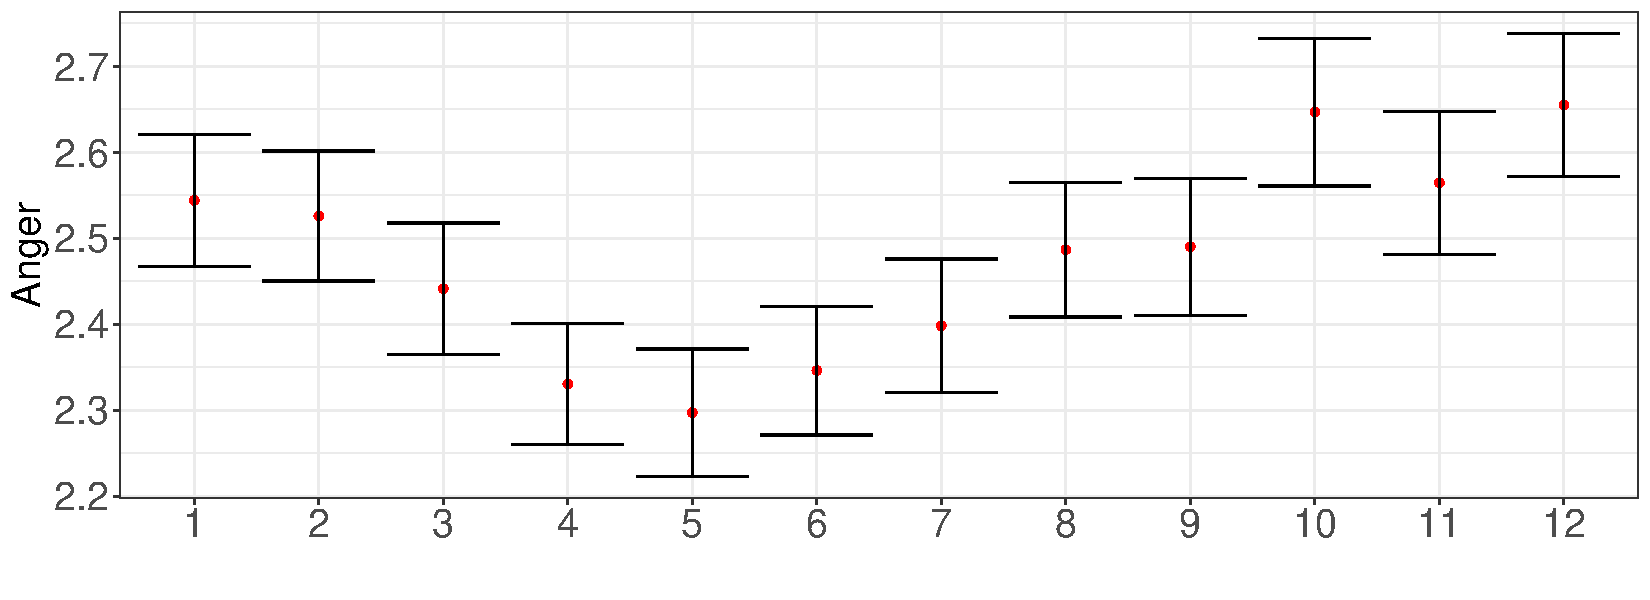
\includegraphics[width=0.98\linewidth]{plots/plt_ang_2} }\newline\subfloat[Anxiety\label{fig:survey-mean-2}]{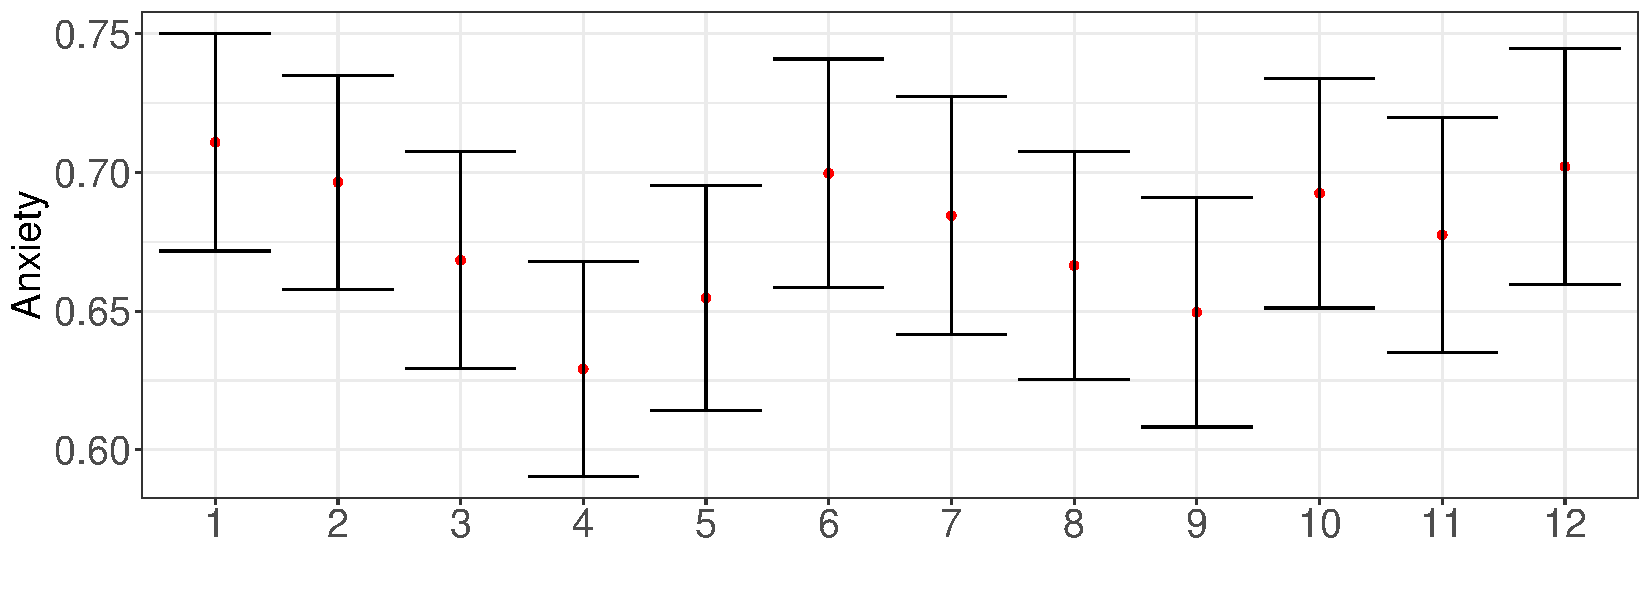
\includegraphics[width=0.98\linewidth]{plots/plt_anx_2} }\newline\subfloat[Depression\label{fig:survey-mean-3}]{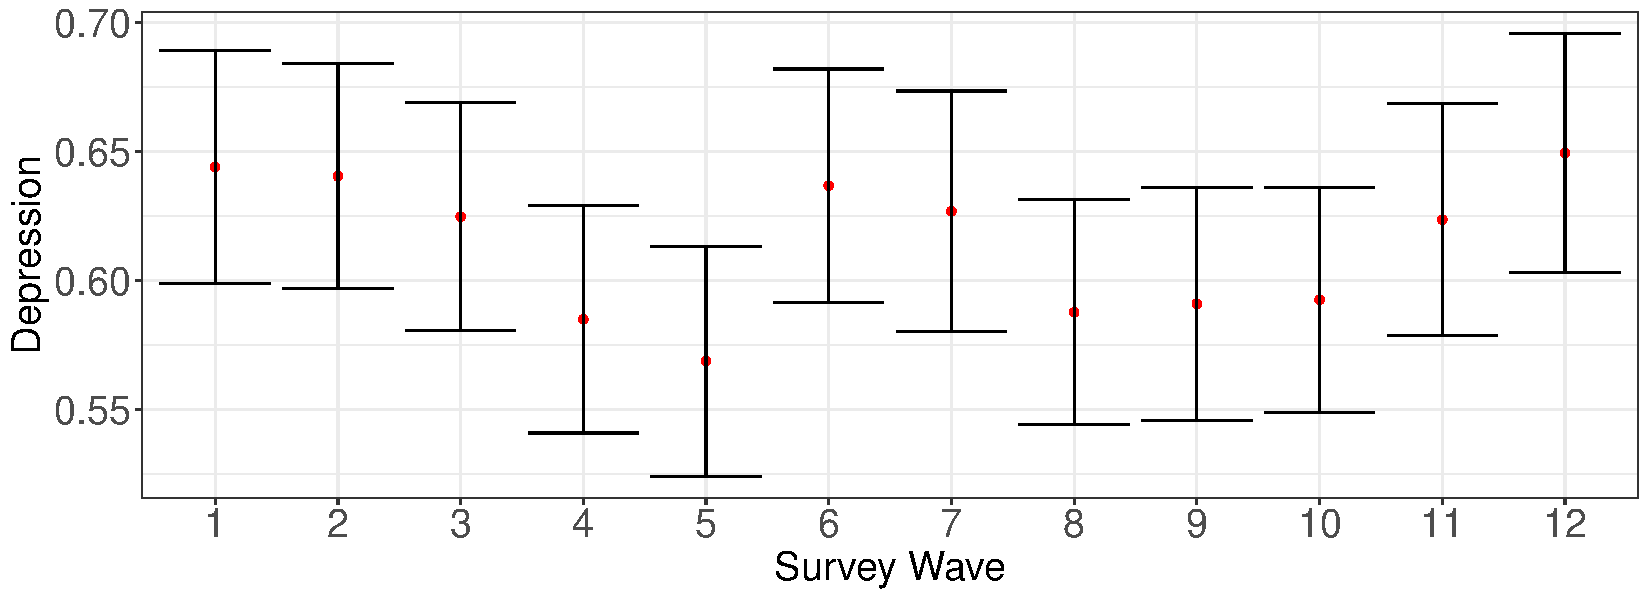
\includegraphics[width=0.98\linewidth]{plots/plt_dep_2} }
\end{figure}

\begin{figure*}
\caption{Three-Day Rolling Means of the LIWC Anger, Anxiety, and Sadness Scores in Twitter and Der Standard in 2020 \label{fig:survey-plot-4}}

\subfloat[Twitter \label{fig:twitter-smooth}]{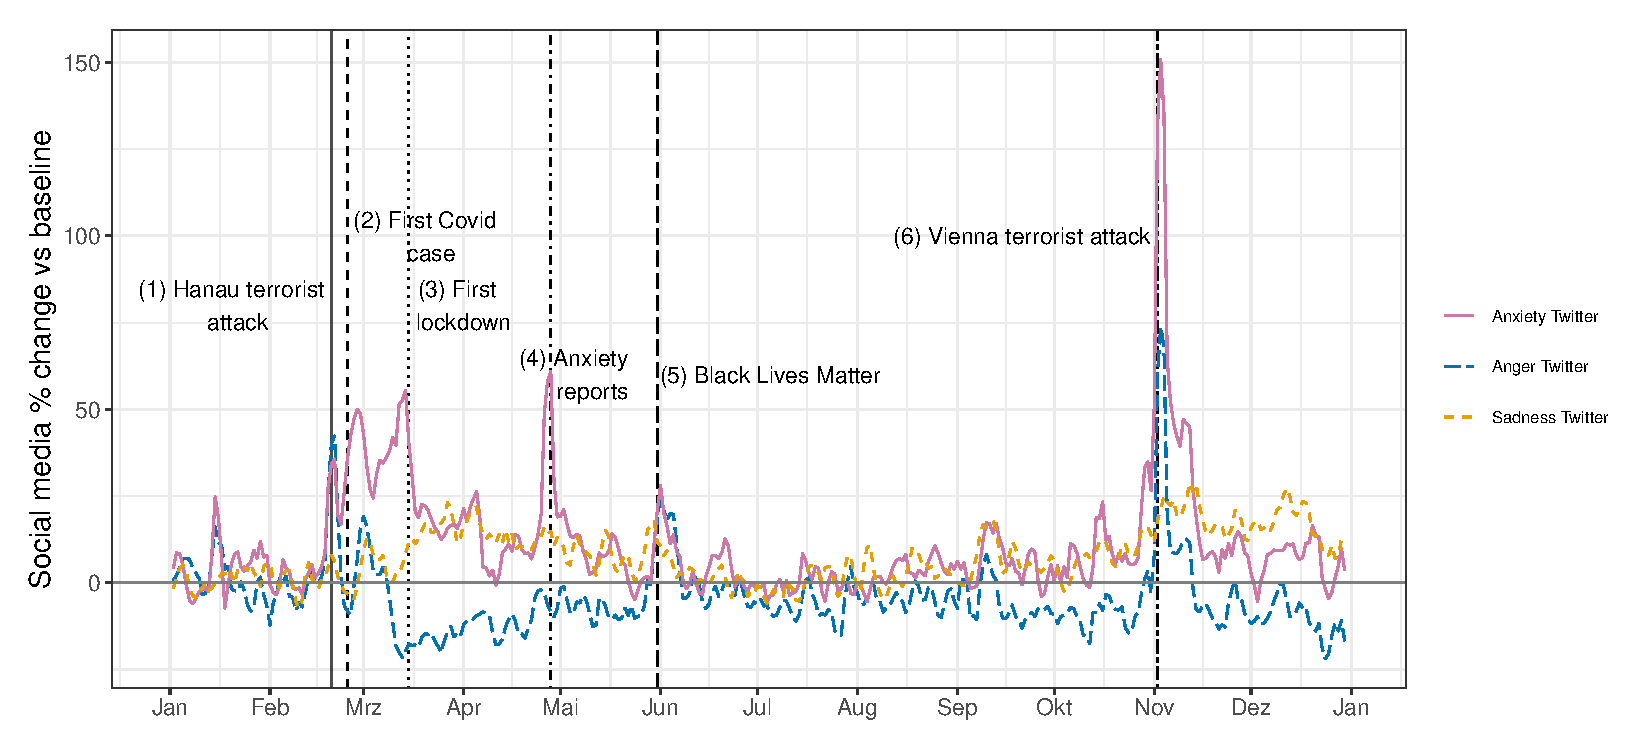
\includegraphics{plots/liwc_twitter_smooth} }\newline\subfloat[Der Standard\label{fig:standard-smooth}]{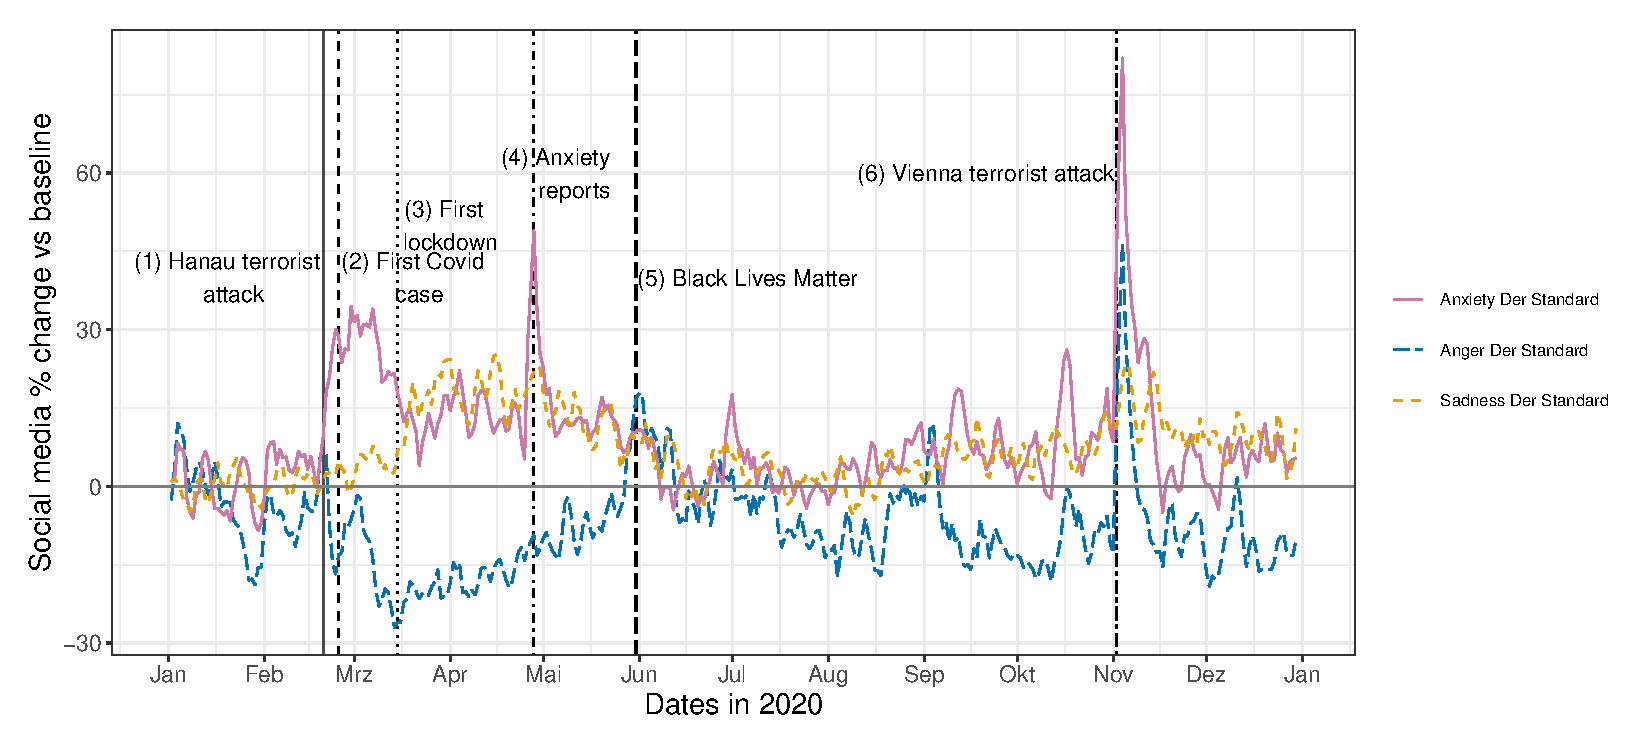
\includegraphics{plots/liwc_standard_smooth}}

\textit{Note:} This plot pictures the three-day rolling means of the baseline-corrected LIWC emotion measures in both social media platforms, Twitter and Der Standard. The vertical lines indicate some of the time points of the following important external events that stirred emotional responses in the Austrian society: (1) the terrorist attack in Hanau, Germany on February 25, 2020, (2) the first Covid-19 case in Austria on February 25, 2020, the first press conference on Covid-19, announcing bans of large public events and university closures as first measures on March 10, 2020, (3) the first death from Covid-19 in Austria on March 12, 2020, followed by strict social distancing measures announced on March 15, 2020, which started on the day after, (4) press releases about considerations of public agencies to stir anxiety of the population at the beginning of the pandemic on April 28, 2020, (5) Black Lives Matter demonstrations against police brutality on May 31, 2020, and (6) the terrorist attack in Vienna, Austria on November 02, 2020.
\end{figure*}

\begin{figure*}
\caption{Spearman's Rank Correlations between Survey Variables and Sentiment Measures \label{fig:survey-plot-6}}
\subfloat[Twitter\label{fig:survey-plot-6-1}]{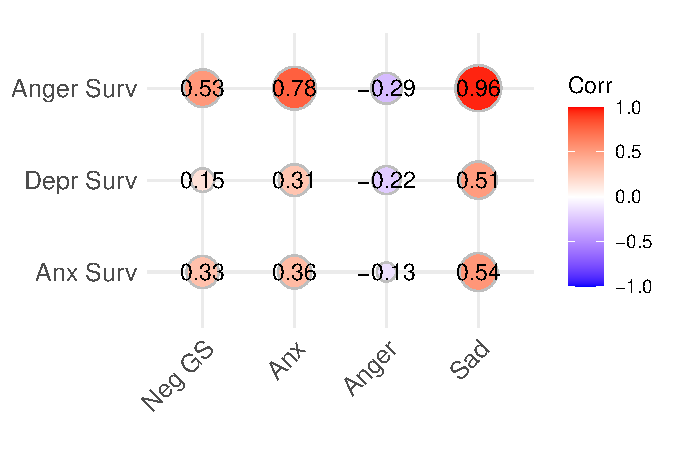
\includegraphics[width=0.48\linewidth]{plots/cortable_twitter} }\subfloat[Der Standard\label{fig:survey-plot-6-2}]{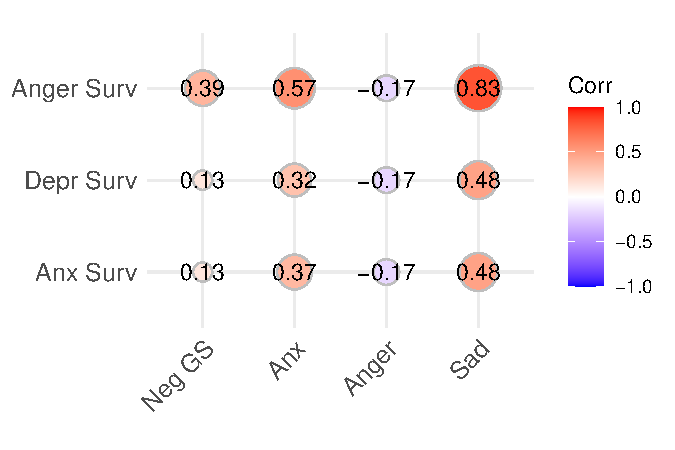
\includegraphics[width=0.48\linewidth]{plots/cortable_stand} }

\textit{Note:} Anx, Anger and Sad stand for the LIWC anxiety, anger, and sadness scores respectively. Neg GS is an abbreviation for the GS negative affect score.
\end{figure*}

\hypertarget{anger}{%
\subsubsection{Anger}\label{anger}}

To test hypotheses 1 (a) and (b) and 4 (a) and (b) we computed Spearman's rank correlations between the anger survey and the LIWC anger score for Twitter and Der Standard, respectively, as well as between the anger survey and the GS negative affect score for both platforms. Levels of significance for all the confirmatory analyses were set by implementing the sequential Holm procedure (Holm, 1979). There was a negative correlation between the corresponding anger scores for both platforms (Twitter: r(10) = -.29 {[}-.73, .30{]}, p = .803, Der Standard: r(10) = -.17 {[}-.65, .41{]}, p = .688). Contrarily, the correlation between the anger survey and the GS negative score was positive, r(10) = .53 {[}-.05, .84{]}, p = .064, and r(10) = .39 {[}-.21, .78{]}, p = .130 respectively. Consequently, we only found the hypothesized positive although insignificant correlation for the machine learning-based negative GS score, and not the dictionary-based anger score.

\hypertarget{anxiety}{%
\subsubsection{Anxiety}\label{anxiety}}

The Spearman's rank correlations between the anxiety survey and the anxiety LIWC score for Twitter and Der Standard were r(10) = .36 {[}-.24, .76{]}, p = .147, and r(10) = .37 {[}-.23, .77{]}, p = .143 respectively. Hence, the corresponding null hypotheses are not rejected although the correlations go in the expected direction.\\
Similarly, the association between the survey anxiety and the GS negative affect score was positive but not significant for either Twitter or Der Standard (r(10) = .33 {[}-.27, .74{]}, p = .171, and r(10) = .13 {[}-.45, .62{]}, p = .357 respectively).

\hypertarget{depression}{%
\subsubsection{Depression}\label{depression}}

Lastly, hypotheses 3 (a) and (b) and 6 (a) and (b) tested the correlation between self-reported depression and LIWC sadness, as well as GS negative affect. The correlation with LIWC sadness was positive for Twitter (r(10) = .51 {[}-.08, .84{]}, p = .071) and Der Standard (r(10) = .48 {[}-.12, .82{]}, p = .086). Similarly, the association between the depression survey and the GS negative affect score was positive for both social media platforms, r(10) = .15 {[}-.42, .64{]}, p = .327, and r(10) = .13 {[}-.45, .62{]}, p = .357. Again, the corresponding null hypotheses cannot be rejected based on this set of data and analyses, although relationships go in the right direction.

\hypertarget{comparison-of-different-confidence-intervals}{%
\subsubsection{Comparison of Different Confidence Intervals}\label{comparison-of-different-confidence-intervals}}

The confidence intervals computed by the analytical approach can be compared to their counterparts computed by the nonparametric bootstrap approach in Table \ref{tab:table-appendix-1} for Twitter and \ref{tab:table-appendix-2} for Der Standard in the Appendix. The results converge in finding non-significant correlations. The corresponding histograms and Q-Q plots of the bootstrap samples are displayed in Figure \ref{fig:survey-plot-7} for Twitter and \ref{fig:survey-plot-8} for Der Standard in the Appendix. It is apparent that with increasing absolute value of \(\rho\) the densities tend to be skewed and consequently less normal. This potentially results in less appropriate estimates with the analytical procedure.

\hypertarget{effect-of-gender-and-federal-state}{%
\subsubsection{Effect of Gender and Federal State}\label{effect-of-gender-and-federal-state}}

Furthermore, we investigated the above associations in more detail for only Twitter data by analyzing the influence of gender and federal state on the link between survey and sentiment scores.
Time series plots of the sentiment measures grouped by gender for two example federal states, Vienna and Upper Austria, illustrate state- and gender-differences in the sentiment scores (Figures \ref{fig:Ang-gender-region}, \ref{fig:Anx-gender-region} and \ref{fig:Sad-gender-region} for LIWC anger, anxiety, and sadness respectively, and Figure \ref{fig:GS-gender-region} for GS negative affect). These plots depict that the variability in Vienna is less pronounced than in Upper Austria, which is a consequence of the much larger sample of tweets from Vienna, leading to more reliable estimates. To investigate if the variability in the sentiment measures significantly improves model performance when controlling for confounding influences of gender and federal state, we employed a hierarchical regression.

\begin{figure*}
\caption{Three-Day Rolling Means of LIWC Anger in Tweets from Users in Vienna and Upper Austria in 2020 Grouped by Gender}\label{fig:Ang-gender-region}
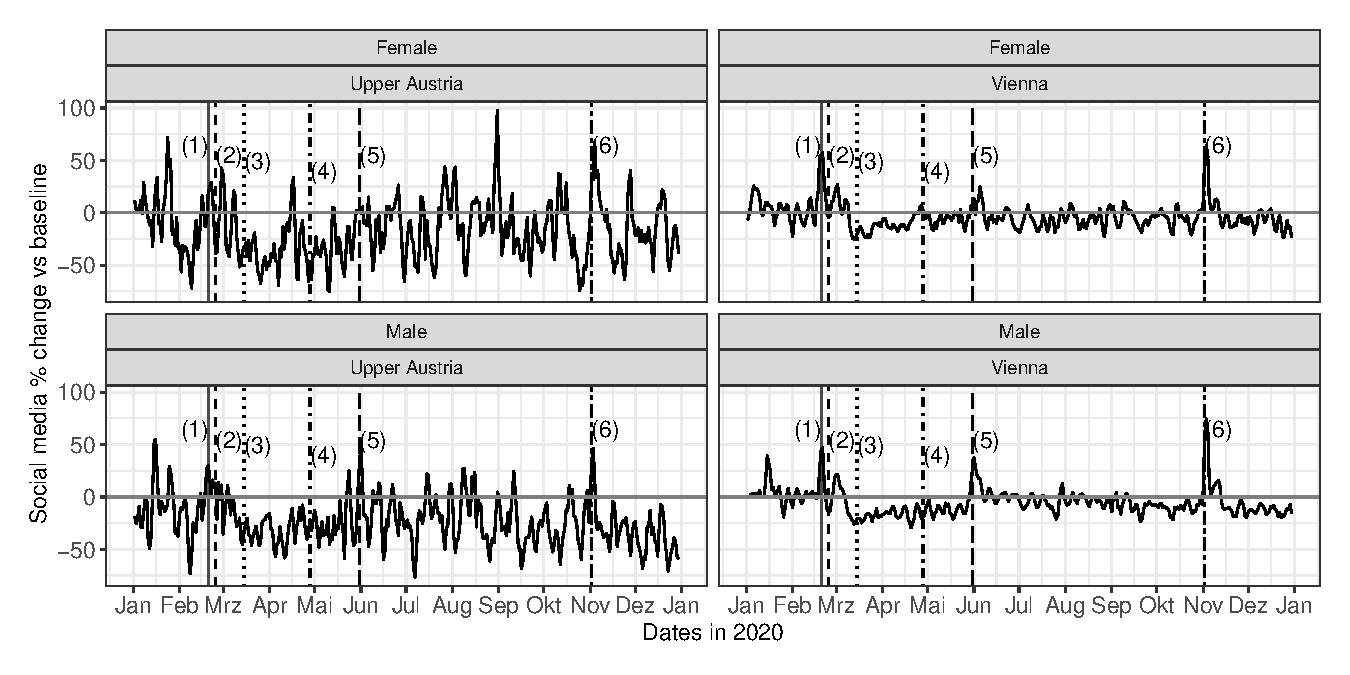
\includegraphics[width=\textwidth]{plots/plt_anger}

\textit{Note:} This plot pictures the three-day rolling means of the baseline-corrected LIWC anger measure in Twitter split by gender and two example federal states, Vienna and Upper Austria. The vertical lines portray important events stirring emotional responses in Austria: (1) the terrorist attack in Hanau, Germany on February 25, 2020, (2) the first Covid-19 case in Austria on February 25, 2020, (3) the first death from Covid-19 in Austria on March 12, 2020, (4) press releases about considerations of public agencies to stir anxiety of the population at the beginning of the pandemic on April 28, 2020, (5) Black Lives Matter demonstrations against police brutality on May 31, 2020, and (6) the terrorist attack in Vienna, Austria on November 02, 2020.
\end{figure*}

Firstly, we computed a regression on survey emotions with only gender and federal state as independent variables. Second, we tested if adding GS negative or the corresponding LIWC score significantly increased model performance.

GS negative affect did not contribute significantly to explaining variation in self-reported anger, \(\Delta R^2 = .01\), 90\% CI \([.00\), \(.06]\), \(F(1, 113) = 1.35\), \(p = .247\). It did also not improve model performance for the anxiety survey measure, \(\Delta R^2 < .01\), 90\% CI \([.00\), \(.03]\), \(F(1, 113) = 0.43\), \(p = .513\). For self-reported depression, \(\Delta R^2 = .03\), 90\% CI \([.00\), \(.09]\), \(F(1, 113) = 7.06\), \(p = .009\) the F-score turned out to be significant. Interestingly, all the coefficients turned out to be negative.
Equivalently, we investigated how the model performance changed when adding the corresponding LIWC emotion to the baseline model. Neither adding LIWC anger nor anxiety improved model performance significantly (\(\Delta R^2 < .01\), 90\% CI \([.00\), \(.03]\), \(F(1, 113) = 0.72\), \(p = .398\) and \(\Delta R^2 = .02\), 90\% CI \([.00\), \(.06]\), \(F(1, 113) = 2.82\), \(p = .096\) respectively). Again, both sentiment score regression coefficients turned out be negative. Contrarily, only the coefficient of LIWC depression was positive as hypothesized and significantly improved model performance when considering the F-score, \(\Delta R^2 = .02\), 90\% CI \([.00\), \(.08]\), \(F(1, 113) = 5.03\), \(p = .027\).
The results of the hierarchical linear regressions are displayed in greater detail in the Appendix in Tables \ref{tab:table-ang-GS} for the survey anger and GS negative affect association, \ref{tab:table-anx-GS} for the survey anxiety and GS negative affect association, \ref{tab:table-depr-GS} for the survey depression and GS negative affect association, \ref{tab:table-ang-liwc} for the survey anger and LIWC anger association, \ref{tab:table-anx-liwc} for the survey anxiety and LIWC anxiety association and \ref{tab:table-depr-liwc} for the survey depression and LIWC sadness association.
Importantly, in all the above analyses most of the variation in the dependent variables are explained by gender and federal state and not by the sentiment measure. \(R^2\) ranges from 0.31 in the baseline models for both self-reported anger models to 0.42 in both self-reported depression baseline models.
The assumptions for these multiple linear regressions are met. See the partial correlation and diagnostic plots in Figure \ref{fig:pcp-plots} and \ref{fig:diagnostic-plots} in the Appendix.

\hypertarget{exploratory-analyses-1}{%
\subsection{Exploratory Analyses}\label{exploratory-analyses-1}}

In order to understand the interrelations between emotional or sentiment and self-reported measures in more detail we conducted further exploratory analyses. Figure \ref{fig:survey-plot-6} provides first insights that it is worth investigating the associations between survey and sentiment measures apart from the ones that were discussed above. Most prominently, whereas the LIWC anger is unexpectedly negatively correlated with self-reported anger, GS negative and LIWC anxiety and sadness exhibit strong positive correlations with the survey measure. This holds true for both social media platforms. It further becomes clear that all three self-reported emotions share a positive correlation with the sentiment measures apart from LIWC anger which consistently is negatively correlated to them. On the one hand, the following section discusses the interrelations between different survey variables and the LIWC and GS measures apart from the main results. On the other hand, we will discuss the influence of changes in the time windows to include the social media data on the relations discussed in the above sections.

\hypertarget{influence-of-time-window-for-sentiment-measures}{%
\subsubsection{Influence of Time Window for Sentiment Measures}\label{influence-of-time-window-for-sentiment-measures}}

Figure \ref{fig:scatter-lag} illustrates how the Spearman's rank correlation coefficients vary as a function of time window before the survey for which we included text data for sentiment measures.
For Twitter, the correlation is in general highest with a time window of only one day prior to each survey wave. The correlation of LIWC sadness with self-reported depression is an exception, being highest from day three to eleven. For Der Standard, all three correlations with GS negative affect are better for windows up to three days. LIWC anger correlates most highly with survey anger for a short one- or two-day window. LIWC sadness correlates most strongly for longer time intervals, similar to Twitter sentiment, increasing slightly from around day seven onward.
Equivalently, Figure \ref{fig:scatter-lag-50} in the Appendix displays the results with the only difference that for each survey wave we only included data of the first \(50\,\%\) of the respondents. The reason for including only the first \(50\,\%\) was to keep the time window more restricted, and thus more comparable to the quickly changing dynamics of the online platforms. The figure looks like Figure \ref{fig:scatter-lag}.

\begin{figure*}
\caption{Spearman's $\rho$ as a Function of the Time Window of Twitter and Der Standard Data Used to Calculate Sentiment Measures}\label{fig:scatter-lag}
\subfloat[Twitter\label{fig:scatter-lag-1}]{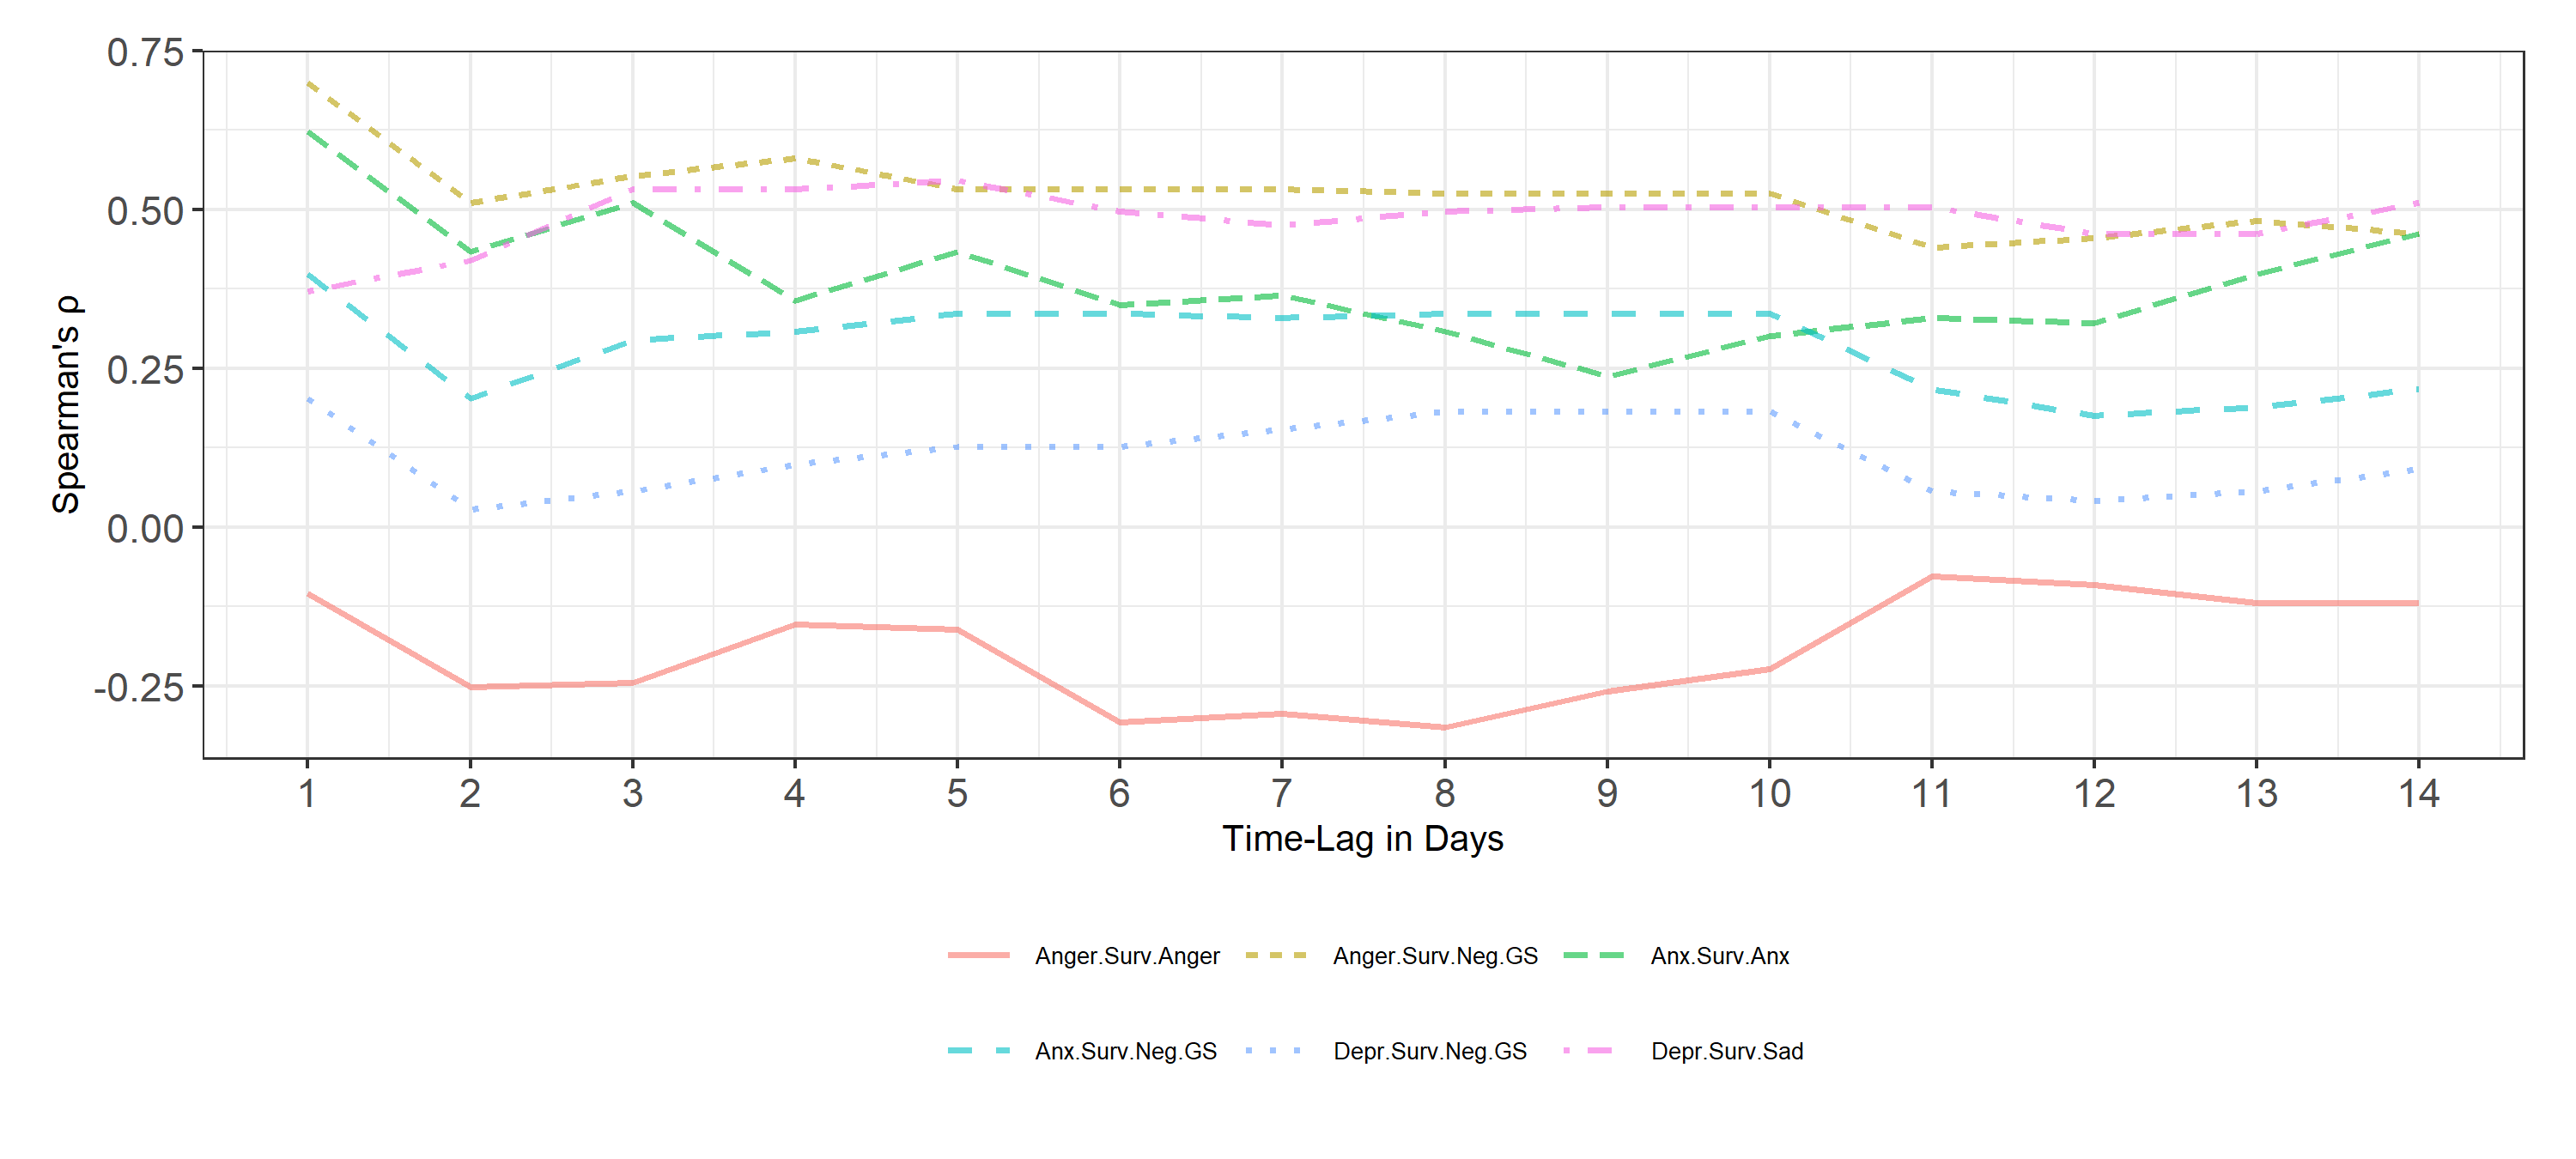
\includegraphics[width=\textwidth]{plots/plt_twitter_lag} }\newline\subfloat[Der Standard\label{fig:scatter-lag-2}]{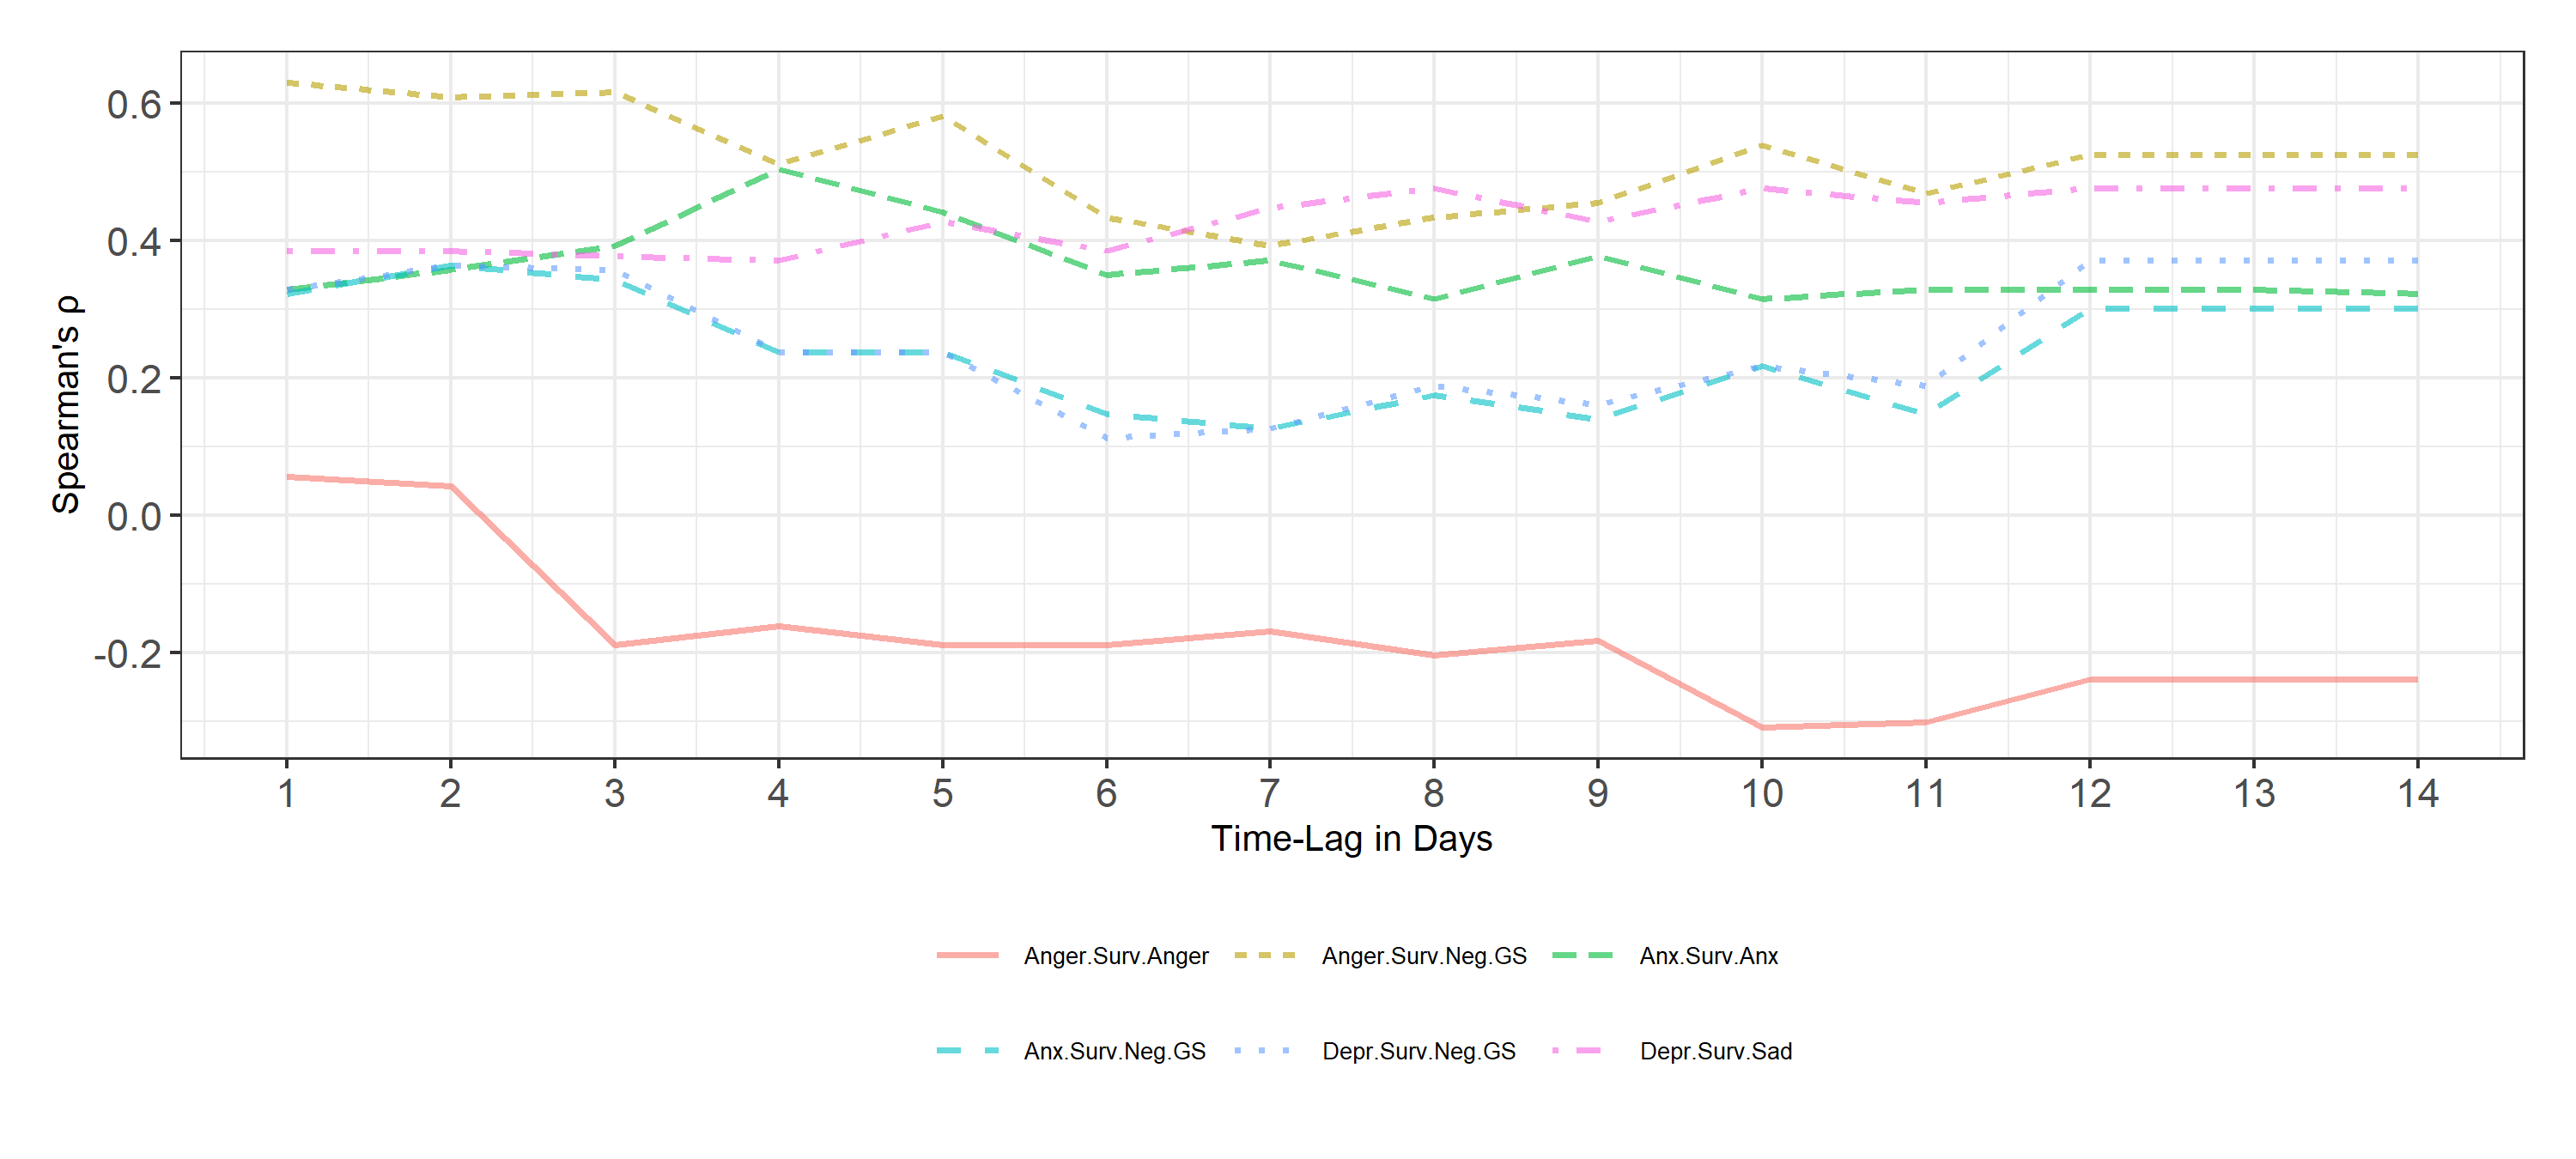
\includegraphics[width=\textwidth]{plots/plt_stand_lag} }


\textit{Note:} This plot depicts the influence of the time window we used to include social media data for the computation of the sentiment measures on the correlation between self-reported and social media sentiment and emotion measures. The motivation behind this analysis is that the survey questions refer back either 14 days in the case of depression or seven days in case of anxiety and anger. To take this into account the start of the time window of included social media data is likewise adopted to either 14 or seven days prior to each survey wave. Past research indicates that the respondent's memory recall might be biased towards more short-termed events. We thus computed correlations based on restricted time windows. Increased correlations with the survey measures for a shorter time window would underline this theory. Note that for anxiety and anger only the correlations for time windows ranging from one to seven days are relevant. For depression the complete range, i.e., from 14 days to one day is relevant.
\end{figure*}

Next, we investigated how the length of the time window influences the regression coefficients of the sentiment measures when additionally controlling for gender and federal state. Figure \ref{fig:coef-lags} depicts the coefficients with corresponding \(95\,\%\) confidence intervals. Interestingly, only the results concerning the coefficients with the LIWC scores converge with the Spearman's rank correlation results. The GS scores however do not exhibit such a consistent pattern. For the survey anger and GS negative relation a restricted time window did not increase the strength of the correlation. The coefficient of the anxiety and GS negative regression is indeed highest with a time window of only one or two days. For depression and GS negative the coefficient also becomes less negative with a restricted time window. Again, it is noteworthy that none of the coefficients related to GS negative exhibits a positive relationship to the survey measure. For the coefficients related to LIWC anger and anxiety however, a restricted time window led to a more positive correlation coefficient. This is especially pronounced for the LIWC anger coefficient. Contrarily, the LIWC sadness coefficient exhibits a reversed pattern. As the time window becomes less restricted the coefficients tend to rise. This indicates that the reference point for the survey depression questions is mirrored better by the sentiment measures when smoothing the data by a greater time interval. Nonetheless, none of the above coefficients vary significantly from each other as a function of the included time window. Yet, this is not surprising giving the small number of survey waves in our dataset.

\begin{figure*}
\caption{Linear Regression Coefficients after Controlling for Gender and federal state as a Function of Time-Window for Twitter Data}\label{fig:coef-lags}
\subfloat[Anger GS Negative\label{fig:survey-plot-7-1}]{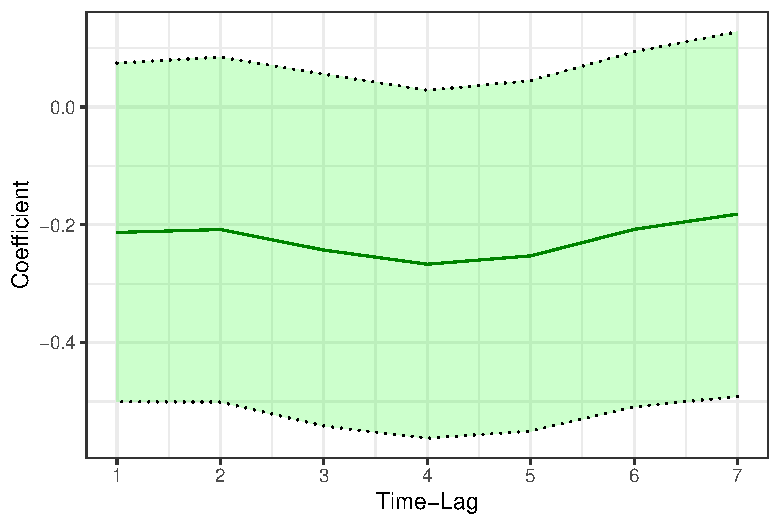
\includegraphics[width=0.48\linewidth]{plots/coef_lags_anger_GS} }\subfloat[Anxiety GS Negative\label{fig:survey-plot-7-2}]{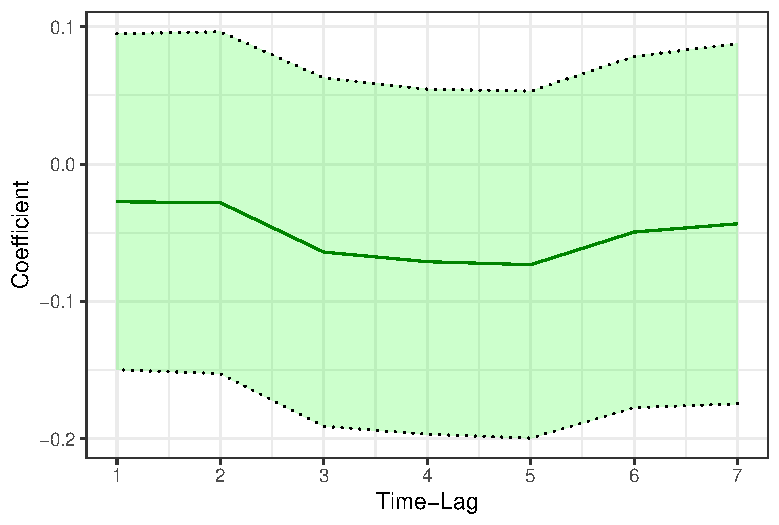
\includegraphics[width=0.48\linewidth]{plots/coef_lags_anxiety_GS} }\newline\subfloat[Depression GS Negative\label{fig:survey-plot-7-3}]{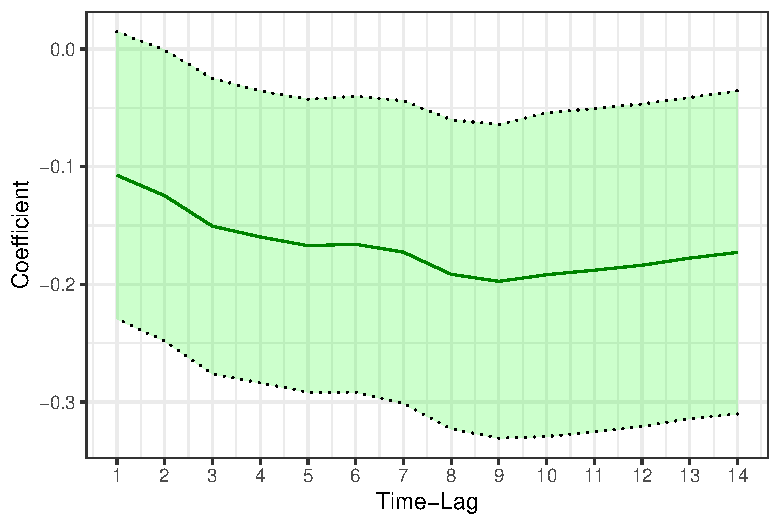
\includegraphics[width=0.48\linewidth]{plots/coef_lags_depr_GS} }\subfloat[Anger LIWC Anger\label{fig:survey-plot-7-4}]{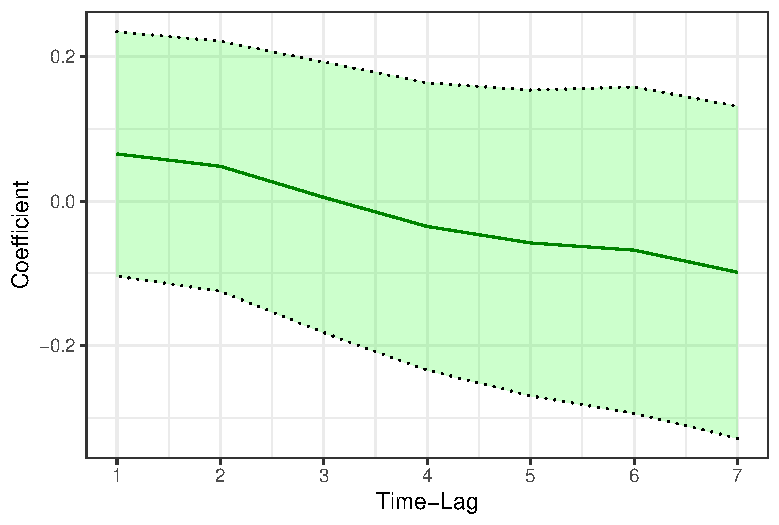
\includegraphics[width=0.48\linewidth]{plots/coef_lags_anger_LIWC} }\newline\subfloat[Anxiety LIWC Anxiety\label{fig:survey-plot-7-5}]{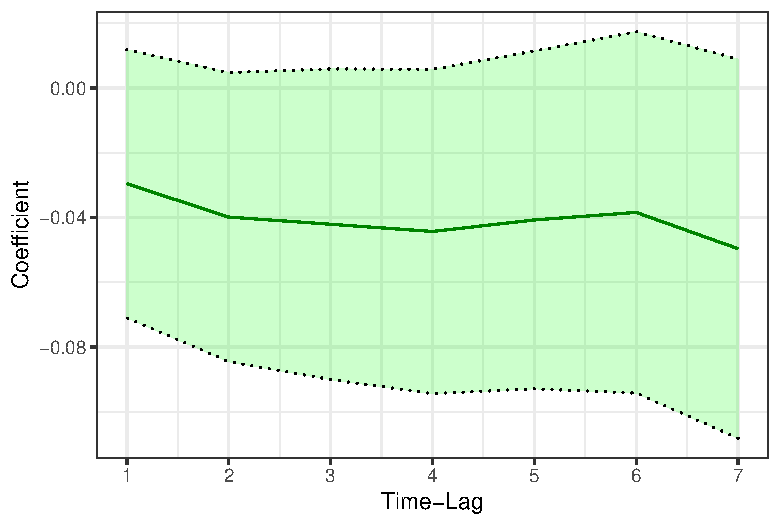
\includegraphics[width=0.48\linewidth]{plots/coef_lags_anxiety_LIWC} }\subfloat[Depression LIWC Sadness\label{fig:survey-plot-7-6}]{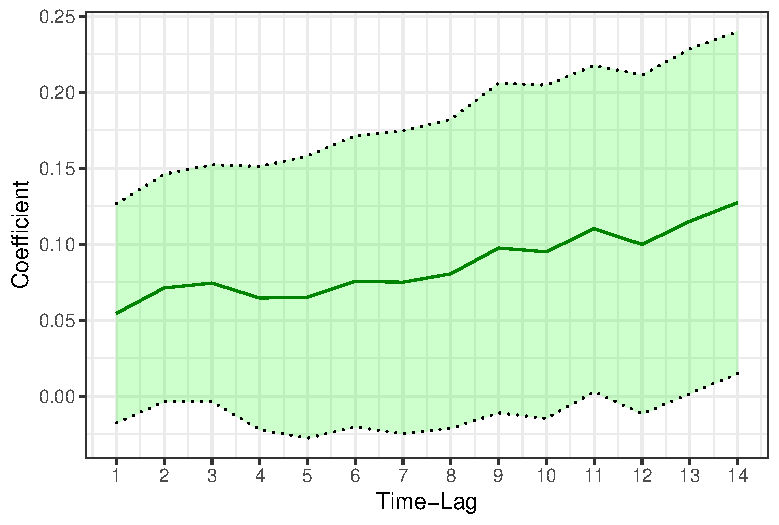
\includegraphics[width=0.48\linewidth]{plots/coef_lags_depr_LIWC} }

\textit{Note:} This plot depicts the influence of the time window we used to include Twitter data for the computation of the sentiment measures on the regression coefficients related to the emotion and sentiment measures. The regression model controlled for the influence of gender and Austrian federal states on the outcome survey measure. The shaded areas around the line depict corresponding 95\,\% confidence intervals. For greater details on the time windows see the note in Figure~\ref{fig:scatter-lag}. Since the anxiety and anger survey questions refer back only seven days the relevant time window range for the corresponding coefficients is from one to seven days.
\end{figure*}

\hypertarget{best-subset-selection-1}{%
\subsubsection{Best Subset Selection}\label{best-subset-selection-1}}

For further exploration we analyzed how different sentiment measures associate with the three survey variables. Figure \ref{fig:survey-plot-6} shows the Spearman's rank correlation coefficients between the survey and sentiment measures. For Twitter, we further employed best subset selection to investigate which combination of independent variables best predicts the different survey variables.
The models that minimize the AIC or BIC for the different survey variables are portrayed in Table \ref{tab:subset}. For a more detailed view of the results Tables \ref{tab:subset-detail}, \ref{tab:subset-detail-2}, \ref{tab:subset-detail-3}, \ref{tab:subset-detail-4}, \ref{tab:subset-detail-5} and \ref{tab:subset-detail-6} in the Appendix list the five winning models for both AIC and BIC for each self-reported measure.

\begin{table*}[h!]

\begin{center}
\begin{threeparttable}

\caption{\label{tab:subset}Resulting Winning Models for the Best Subset Selection that Minimize AIC or BIC for the Different Survey Variable}

\small{

\begin{tabular}{llllllllllllll}
\toprule
 & \multicolumn{1}{c}{Salz} & \multicolumn{1}{c}{Styr} & \multicolumn{1}{c}{Tyr} & \multicolumn{1}{c}{Vie} & \multicolumn{1}{c}{Male} & \multicolumn{1}{c}{LI Pos} & \multicolumn{1}{c}{LI Neg} & \multicolumn{1}{c}{LI Anx} & \multicolumn{1}{c}{LI Ang} & \multicolumn{1}{c}{LI Sad} & \multicolumn{1}{c}{GS Pos} & \multicolumn{1}{c}{GS Neg} & \multicolumn{1}{c}{IC}\\
\midrule
Ang AIC & 0.18 & - & - & - & -0.29 & 0.14 & - & - & -0.32 & 0.59 & -0.19 & - & -384.78\\
Ang BIC & 0.15 & - & - & - & -0.30 & - & - & - & -0.33 & 0.68 & - & - & -370.18\\
Anx AIC & 0.06 & - & 0.05 & -0.06 & -0.12 & - & 0.18 & -0.06 & - & - & - & - & -571.09\\
Anx BIC & 0.09 & - & 0.06 & - & -0.12 & - & - & - & - & - & - & - & -559.83\\
Depr AIC & 0.12 & 0.06 & - & -0.03 & -0.17 & - & 0.44 & -0.11 & -0.20 & - & - & -0.17 & -580.34\\
Depr BIC & 0.07 & - & - & - & -0.15 & 0.23 & - & - & - & - & - & - & -567.20\\
\bottomrule
\addlinespace
\end{tabular}

}

\begin{tablenotes}[para]
\normalsize{\textit{Note.} Salz, Styr, Tyr and Vie are abbreviations for Salzburg, Styria, Tyrol and Vienna. LI, Pos, Neg, Anx, Ang and Depr are the respective abbreviations for LIWC, positive, negative, anxiety, anger and depression. Variables that were not included in a model were labelled with a hyphen. The last column always displays the respective information criterion - either AIC or BIC.}
\end{tablenotes}

\end{threeparttable}
\end{center}

\end{table*}

First, the winning models for AIC and BIC do not converge in selecting the exact same model. Unsurprisingly, BIC selects models with a smaller number of independent variables. However, the winning models per self-reported measure consistently include similar variables. Second, whenever one of the winning models contains LIWC positive emotion, its regression coefficient is positive. This indicates that the LIWC positive emotion score is an important factor in reducing AIC and BIC and hence increasing model performance in explaining self-reported depression and anger.
Third, winning models including LIWC negative emotion also include LIWC anxiety and anger or only LIWC anxiety. Whereas LIWC negative emotion yields a positive regression coefficient, the corresponding anger and anxiety coefficients are negative. This phenomenon is especially pronounced in the winning models for the self-reported depression variable.
Importantly, these coefficients are difficult to interpret since LIWC negative is a linear combination of LIWC anger, anxiety and sadness and hence is associated with these emotions by definition. Potentially, the positive LIWC negative affect score reflects a high influence of LIWC sadness that is reduced by LIWC anxiety and anger. Practically, people who score high in self-reported depression tend to use fewer words indicating anxiety or anger but more sadness-related words. In comparison, the self-reported anger models only include LIWC anger and sadness. In this case, the coefficient for LIWC anger is again negative while the one for LIWC sadness is positive which supports the interpretation.
Fourth, similar to the hierarchical regressions, GS negative affect is negatively associated with the dependent survey measures. Again, this phenomenon is strongest in the case of the depression survey variable. This indicates that negative affect GS captures negative emotionality apart from the one primarily present in depression.
Fifth, the corresponding LIWC emotion (e.g., LIWC anger in the anger survey regressions) is always integrated in a winning model at least once but does not always yield an expected positive regression coefficient. As was demonstrated in the analyses above, especially the LIWC anger construct is negatively associated with the corresponding survey measure. The same effect is present for anxiety but less pronounced. Only for the depression survey variable two of the winning BIC models indicate a positive linear association with the LIWC sadness variable when controlling for the other included independent measures (compare with Table \ref{tab:subset-detail-6} in the Appendix).
Furthermore, the effects of LIWC sadness and GS positive in the winning anger survey models are worth investigating. While LIWC sadness has a relatively high positive regression coefficient, the regression coefficient of GS positive is consistently negative throughout all models that included this variable.
Lastly Table \ref{tab:subset} indicates that differences between certain federal states do not add to the model's explanatory power and are therefore not included in the winning models. Hence, some federal states seem not to differ strongly in their self-reported or social media measure from the baseline federal state, i.e., Upper Austria. Strong differences here would also have been hard to explain.

It is important to mention that issues of multicollinearity might limit the efficiency of parameter estimation when multiple survey measures are added to a model.

\hypertarget{mixed-factor-analysis-and-multiple-linear-regression-1}{%
\subsubsection{Mixed Factor Analysis and Multiple Linear Regression}\label{mixed-factor-analysis-and-multiple-linear-regression-1}}

\begin{figure*}[h!b]
\caption{Spearman's $\rho$ between Twitter and Der Standard Emotion and Sentiment Measures and the Resulting Factor Scores}\label{fig:spear-fa}
\subfloat[Twitter\label{fig:spear-fa-1}]{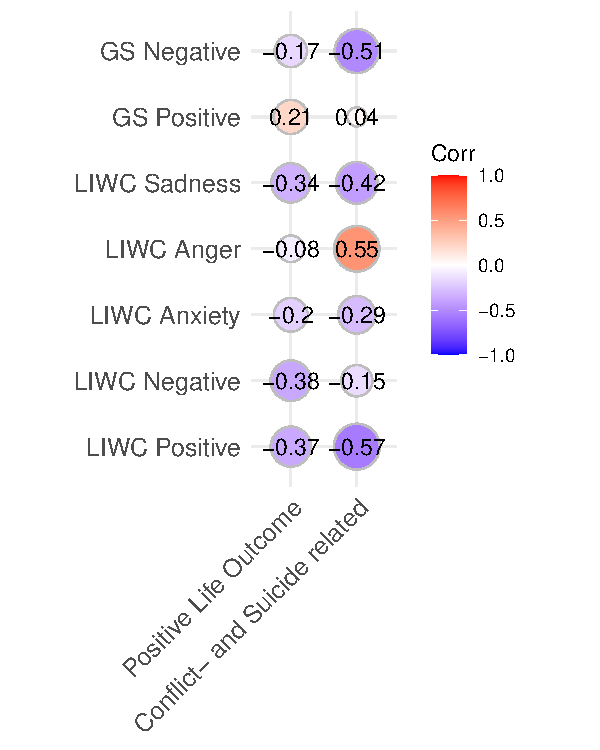
\includegraphics[width=0.48\linewidth]{plots/plot_spear_fa_twitter} }\subfloat[Der Standard\label{fig:spear-fa-2}]{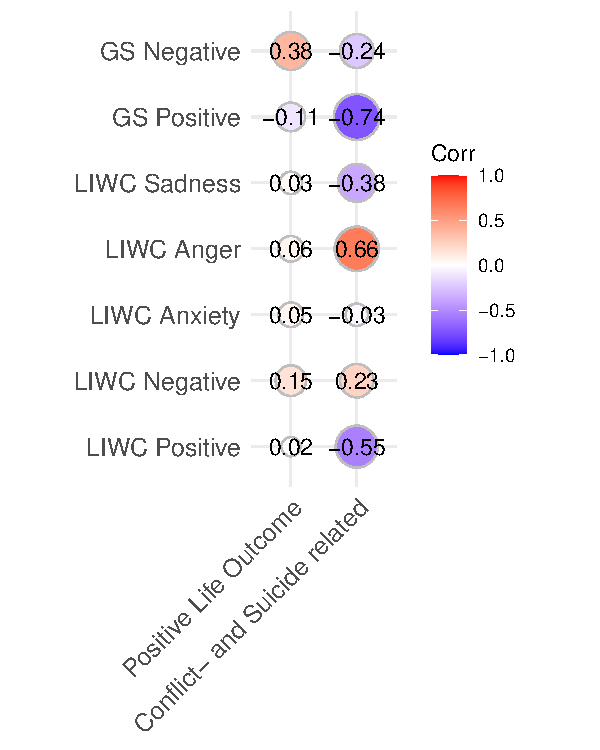
\includegraphics[width=0.48\linewidth]{plots/plot_spear_fa_stand} }
\end{figure*}

To investigate how further survey variables beyond anger, anxiety and depression are associated with different sentiment measures we employed a factor analysis on the tetrachoric and polychoric correlations. The included variables ranged from diverse conflict-related variables (i.e., conflict with family or partner, conflict at work, experience of psychological or physical domestic violence and change of conflicts versus pre-Covid times) to suicidal ideation and various variables assessing positive life outcomes compared to pre-Covid. Figure \ref{fig:table-mix-cor} portrays the corresponding mixed correlations between the included variables.
Figure \ref{fig:scree-plot} in the Appendix depicts the scree plots, additionally indicating the results of the parallel analysis to decide on the number of factors to compute the analysis with. Even though the parallel analysis suggested six factors we adhered to the scree plot and Kaiser criterion, which converged towards a factor analysis with two factors. This further allowed for an easier interpretation. Furthermore, the mixed correlation table depicts two clusters of variables that are positively correlated with each other. The first cluster consists of the positive life outcomes which consistently positively correlate with each other. Contrarily, the second cluster consists of the conflict-, violence- and suicide-related variables.
Resulting loading structures and variable communalities of the factor analysis after varimax rotation are portrayed in Table \ref{tab:loading} in the Appendix.
Communalities are the sum of the squared factor loadings for each variable. In total, this model accounted for 42\(\,\%\) of the variance. The first factor explains 60\(\,\%\) of this variance, while the second factor accounts for the remaining 40\(\,\%\).
Based on the factor loadings of the variables, the two factors were interpreted as a conflict- and suicide-related score and a positive life outcome score.
The former factor scores consistently high on the conflict-, violence- and suicide-related variables. Contrarily, the second factor scores high on the positive life outcomes. Hence it mirrors the cluster structure described above which is present in the mixed correlation table (see Figure \ref{fig:table-mix-cor}). We computed Spearman's rank correlations to investigate the interrelations between resulting factor scores and emotion and sentiment measures. Figure \ref{fig:spear-fa} portrays these correlations.
Concerning the correlations of factor scores with the sentiment measures on Twitter, the positive life outcome score was negatively correlated with the LIWC and GS negative. As expected, GS positive was positively correlated with the life outcome score. Surprisingly, this score exhibited a strong negative correlation with LIWC positive. This indicates that a greater number of words associated with positive emotions or meaning were present in social media whilst positive life outcomes tended to decrease compared to pre-Covid times.
Interestingly, for Twitter, the conflict- and suicide-related score exhibits a similar correlation pattern to the other score at first glance. Importantly, once again the LIWC positive is negatively correlated with the conflict- and suicide-related score. Whereas this factor score exhibits a plausible positive correlation with LIWC anger, it was unintuitively negatively correlated to LIWC anxiety and sadness, and most prominently, GS negative.
In the Der Standard data, the positive life outcome score is uncorrelated with most of the emotion and sentiment scores, except for a positive correlation with GS negative. The correlation of the score related to positive life outcomes with LIWC positive is negative for Twitter while the variables are uncorrelated for Der Standard.
But unlike with Twitter, it exhibits an implausible higher positive correlation with the LIWC negative affect score as well as with the sentiment anger score. Again, the unexpected negative correlation with the social media sadness score is still present. Remarkably, the conflict- and suicide-related factor score is negatively correlated with the GS negative affect score, even though to a lesser degree than for Twitter. There is a great difference between Twitter and Der Standard for this factor's correlation with the GS positive affect score. Here, a strong negative correlation is apparent. Likewise, it is more strongly positively correlated with the LIWC anger score.

\hypertarget{discussion}{%
\section{Discussion}\label{discussion}}

Understanding the emotional changes in a society in the context of a pandemic is essential knowledge to adapt public health resources or to inform crisis communication. A promising tool to measure emotional trends in society at large is the processing of social media data. Fast and easy access to live large-scale data is a promise that public health stakeholders traditionally struggled to achieve. Assessing the quality of social media emotion measures is crucial for researchers and stakeholders alike to choose reliable and valid tools. This study therefore investigated whether leveraging social media data provides a similar picture of a population's emotional state compared to surveying mental health-related information -- the latter being costly and effortful to conduct. To assess this research question, we analyzed associations between self-reported emotion and mental health variables and related sentiment measures. We compared two different text analysis tools: a dictionary approach (LIWC) and a machine learning approach (GS), which both measure negative and positive sentiment. Additionally, LIWC can also differentiate between three negative emotions: anger, anxiety and sadness.
Besides the LIWC anger dictionary, both LIWC and GS measures were positively related to the corresponding self-reported emotions, although insignificantly.
Furthermore, we evaluated further correlations of different sentiment measures with the self-reported anger, anxiety, and depression variables, e.g., how the LIWC sadness links to self-reported anxiety and anger (see Figure \ref{fig:survey-plot-6}).
Also, for this set of correlations only the association concerning LIWC anger were negative. All other correlations were positive. Especially self-reported anger correlated highly with LIWC anxiety and sadness.
For Twitter we could follow up on these findings by analyzing to what degree the relation is confounded by gender and federal state. Surprisingly, after controlling for the demographic variables, only the association between LIWC sadness and self-reported depression remained positive. Our results suggest that most of the explained variation in the survey variables are due to variation in gender and federal state. This is supported by the results of the best subset selection. Every model minimizing the information criteria includes gender and at least one federal state. More specifically, the regression coefficients from both the hierarchical regression analyses and best subset selection inform us that differences in gender are more influential in explaining this effect. The corresponding regression coefficient is approximately twice as large for gender.\\
This means that gender is a better predictor for how people feel rather than the tweets they write, i.e., their opinions and thoughts about daily events. Federal state on the contrary is harder to interpret since it itself might be confounded by age, education, or income.
Indeed, the linear associations between social media and survey emotions was seldom positive after controlling for the demographic variables. When they were positive the performance of the model just increased slightly. Hence, the monotonic relations captured by the correlations are potentially also heavily confounded by variation in gender and federal state.\\
Therefore, the results do not indicate a one-to-one mapping between the current survey and both social media platforms. Nevertheless, the present study's results are interesting in various regards.

\hypertarget{comparisons-with-previous-studies}{%
\subsection{Comparisons with Previous Studies}\label{comparisons-with-previous-studies}}

As mentioned above, all the corresponding survey and social media measures' Spearman's rank correlation coefficients are positive but for the association with LIWC anger. Consequently, the present results partly support recent research on the topic that followed a similar methodology (Garcia et al., 2021; Jaidka et al., 2020; Pellert et al., 2021). These studies stress existing substantial correlations between various self-reported emotions and online emotion and sentiment measures.
Pellert et al. (2021) analyzed associations between self-reported positive or negative sentiment assessed on the Der Standard's website with corresponding sentiment measures on Twitter and Der Standard in Austria. Therefore, their analyses focus on German text. They measured participants' feelings about the past day with one simple item. The answers ranged from positive to negative on a four-point scale. They then focused on the daily fraction of reported positive emotions. The authors employed the same methods as the current study: LIWC as an example of a dictionary-based and GS as a machine learning-based tool. Their study differed from the present study regarding the resolution of the self-reports and the representative of the survey. The survey measure had a daily resolution lasting for 20 days in total and was non-representative since the self-reports were assessed on the same platform as one of the social media data sources.
Garcia et al. (2021) compared week to week emotional data of a representative UK survey with seven days rolling means of corresponding social media measures.
The UK survey included a timespan of two consecutive years and resembles our anxiety and anger items, which also comprised a weekly reference timespan. More specifically, the authors mainly focused on three self-reported measures and their associations to a dictionary-based and machine learning-based emotion measure in English language on Twitter. Firstly, they analyzed the association between self-reported anxiety and anxiety LIWC or a fear-related machine learning measure. Second, they investigated the link between self-reported sadness and matching LIWC or machine learning-based measures. Third, Garcia et al. (2021) scrutinized the relation between happiness in the survey and positive LIWC or a joy-related machine learning measure. Compared to the present study, the authors employed a different emotion-based machine learning tool.
The analyses of Jaidka et al. (2020) focused on English postings on Reddit in the US. In contrast to the other two studies, they analyzed cross-regional differences rather than longitudinal changes. Also, the authors investigated the correlation between survey and social media concerning long-term variables like life satisfaction. Besides life satisfaction, they analyzed associations between happiness, worry and sadness in the survey and different social media measures. Compared to Garcia et al. (2021), also self-reported happiness refers to an emotional state that is more long-term than the one assessed by self-reported joy. The yearly survey resolution in their study also point to the long-term character of their variables in contrast to the other two studies. Jaidka et al. (2020) employed various dictionary-based - among others positive and negative LIWC - and machine learning-based analysis tools.
Specifically, the higher time resolution and the matching survey and social media user population in the study by Pellert et al. (2021) potentially explains the higher correlation coefficient of the survey and social media measures compared to the results presented by Garcia et al. (2021), Jaidka et al. (2020) and us. The present study extents the research focus to whether we can observe similar associations with self-reported data assessed by a representative Austrian survey. It further included a question about anger, which has not been investigated in these earlier studies. Importantly, while we assessed self-reported anger by one item similarly to Pellert et al. (2021), self-reported anxiety and depression measured more latent and complex mental health constructs by multiple items, rather than a specific emotion. The anger and anxiety items referred to the respondent's state of anger and anxiety in the past week. The depression item was interested in a comparably long-term mental health state and referred to the past two weeks.
All the above studies focused on a time period in which Covid-19 dominated public dispute.
When compared in more detail our results do not completely converge with these studies. Protruding differences and similarities in the design and results compared to the present thesis are discussed thoroughly in the following.

\hypertarget{machine-learning-based-vs.-dictionary-based-sentiment-measures}{%
\subsubsection{Machine Learning-Based vs.~Dictionary-Based Sentiment Measures}\label{machine-learning-based-vs.-dictionary-based-sentiment-measures}}

The results presented by Garcia et al. (2021), Jaidka et al. (2020) and Pellert et al. (2021) all found that machine learning-methods were more robust than dictionary-based methods when considering correlations with self-reported positive emotions. In the study by Jaidka et al. (2020) the performance of the two methods differed substantially. While the machine learning-based measure was consistently positively or negatively associated to respective self-reported measures, dictionary-based measures exhibited the reversed pattern. Pellert et al. (2021) found that both LIWC and GS positive correlated positively with self-reported positive affect. GS positive exhibited a stronger association. However, the results presented by Pellert et al. (2021) are inconsistent when evaluating how LIWC and GS negative affect correlates with surveyed positivity. For Der Standard only, GS exhibited expected negative correlations while LIWC negative was uncorrelated to the survey variable. For Twitter, GS was still negatively correlated with the self-reported measure, but LIWC negative outperformed the machine learning-based measure. Contrarily, the study of Garcia et al. (2021) found no substantial differences between both sentiment measures' performance when considering survey sadness and anxiety. Yet, as in the other studies, machine learning-based methods outperformed LIWC positive in correlating with self-reported joy. Given that the machine learning model specifically predicted joy, while LIWC captures all kinds of positive expressions, this hints again that the close similarity between survey and social media measures improves performance.
The present study's main results indicate that machine learning (GS) qualitatively and quantitatively outperforms the LIWC dictionary method in the case of anger. People who reported to feel angry possibly tend to use language that reflects negative affect per se but may not explicitly use more anger-related words. GS negative on social media is positively correlated to self-reported anger in contrast to LIWC anger, which results in a negative association. For survey depression, however, the sadness dictionary fared better and produced higher positive associations than GS negative. Potentially, GS negative covers a wide range of negative emotions that are not primarily present in depression. Sadness on the contrary is hypothesized to transform to depression when avoidance behavior is present for a prolonged timespan (Leventhal, 2008) and is consequently closely linked to depression. Therefore, indications of sadness might be identifiable in social media language of people struggling with symptoms of depression. The result is supported by the hierarchical regression results. When controlling for gender and federal state, the correlation of depression with GS negative was negative but remained positive for LIWC sadness.\\
Moreover, selecting the best subset based on the AIC criterion shows that the winning models included LIWC and GS positive for self-reported anger, and LIWC and GS negative for self-reported depression. Both LIWC and GS - although intended to measure positive affect - seem to capture different emotional aspects. Machine learning-based and dictionary-based methods hence might be more informative when employed in union. Pellert et al. (2021) support this hypothesis: The average between corresponding LIWC and GS scores outperformed the single measures in most cases. In general, people may talk more about some emotions than about others, for example, more about sadness than about anger. Our study, together with previous results, could indicate that sadness and some positive emotions like joy can be assessed using social media data, while anger is harder to measure.

\hypertarget{positive-and-negative-life-events-and-emotions}{%
\subsubsection{Positive and Negative Life Events and Emotions}\label{positive-and-negative-life-events-and-emotions}}

In order to understand the relation between survey variables and sentiment measures better we computed a factor analysis with various survey variables. The two-factor solution consisted of a conflict- and suicide-related and a positive life outcome-related score. These scores were correlated with some of the online emotion measures. Similar to Pellert et al. (2021), the positive life outcome score assessed a positive emotional state with the only difference that it is more long-term in the current case. This factor score was negatively related to both LIWC and GS negative only in Twitter as in the study by Pellert et al. (2021). For Der Standard, we unexpectedly observed negative correlations. The Der Standard online forum consists of comments below news tickers and published articles. Thus, these postings are rather about news and less about personal experiences. On Twitter, postings may cover a wider range of subjects and hence allow to capture signals related to the conflict-, suicide- or positive life outcome-related variables.
Future research should assess how language and topics qualitatively differ between these platforms and whether, for example, emotions are transported in higher-level contexts that rely on a sentence or text but not so heavily on a word level.
Furthermore, we found that LIWC positive is negatively correlated to the conflict- and suicide-related score. This suggests that the absence of words related to positive emotions indicates a rise in such negative life events. For the case of Der Standard also GS positive negatively correlates with the conflict- and suicide-related factor score. Language related to positive emotions - on a word level as assessed by the LIWC and on a context-dependent sentence level as assessed by the GS - might therefore be scarce at times when negative life events are more present in the population. The result, however, needs replication and is also not entirely supported for Twitter where GS positive is uncorrelated to the conflict- and suicide-related factor score.
Interestingly, reports of conflict- and suicide-related events tend to increase when the use of anger-related words increases. Yet, they generally decrease with or are not correlated to a rise in other social media measures related to negative affect. At least for Twitter, our results hence point to a less emotional language in general, but more anger, at times of conflicts, violence, or suicidal thoughts. Indeed, the result is supported by research showing that women who experienced domestic violence tend to feel angrier and more apathetic (Avdibegovic et al., 2017).
Additionally, the positive life outcome score was negatively correlated or uncorrelated to LIWC positive in Twitter and Der Standard, respectively. Jaidka et al. (2020) discussed similar results: LIWC positive as well as other dictionary-based methods were negatively correlated or uncorrelated to life satisfaction and happiness. LIWC positive includes a broad class of positive words, ranging from \emph{good}, \emph{better}, \emph{love} to \emph{like}. The use of these words does not necessarily express an emotion. Jaidka et al. (2020) investigated this phenomenon further and found that positive affect in social media is dominated by a few words (especially \emph{lol}, \emph{lmao}, \emph{lmfao} or \emph{love}) that correlate negatively with self-reported life satisfaction. Especially the three former words do not express positive emotions but rather irony. Interestingly, when excluding these words, the correlation became less negative or even positive. Future work could check whether this also holds true for the current set of German data. The best subset selection likewise reflects this ambiguity concerning LIWC positive. LIWC positive consistently correlates positively with both self-reported anger and depression. Contrarily, GS positive is negatively correlated with self-reported anger and hence might represent positive emotions more accurately.

\hypertarget{importance-of-the-dependent-measure}{%
\subsubsection{Importance of the Dependent Measure}\label{importance-of-the-dependent-measure}}

Moreover, the studies differ in their dependent survey measures. As discussed by Pellert et al. (2021), the strength of the association between survey and social media measures potentially varies as a function of the volatility of certain emotional variables. Variables which do not change rapidly may not be well represented in the volatile emotional trends on social media. Contrarily, fast-changing emotional experiences that for instance evolve on a day-to-day basis as reaction to external shocks are captured more accurately and hence correlate more highly.
On Twitter and Der Standard, people primarily discuss political events and the news of the day, but not their mental health. Metzler et al. (2021) illustrated that non-emotional words prior to the Covid-19 pandemic were often related to politics and then shifted to Covid-19-related topics as soon as the pandemic unfolded. Importantly, the sentiment measures' variations are systematic and seem to measure some kind of emotional reaction to external events as indicated in the time series plots in Figure \ref{fig:survey-plot-4}. This is also not a platform effect since the LIWC and GS scores vary consistently across Twitter and Der Standard. In contrast to this, the survey by Niederkrotenthaler et al. (2022) mainly assessed mental health indicators, which we correlated with the social media emotion and sentiment measures.
Mental health is a more long-term variable, whereas the expression of emotions on social media about recent events are short-lived. Hence, the survey is not as strongly related to everyday news as people's emotional reactions on Twitter and Der Standard. This might explain the drop in correlational strength we observed in the current study especially compared to Pellert et al. (2021).
Therefore, what the LIWC and GS measures assess differs from the survey questions. Social media data might allow capturing fear towards an external event, e.g., a virus or war, whereas survey measures provide a measure of anxiety that is not necessarily directed towards a specific event. Rather, the anxiety questionnaire HADS (Zigmond \& Snaith, 1983) can also assess feelings of inexplicable unease that potentially are less prominent and explicit in social media postings. Generally, whereas the respondents must self-consciously infer their own feelings to respond to the survey, emotion and sentiment measures on social media can only capture expressed emotions.
Taken together, the set of studies discussed here may show that fast-evolving emotions are better reflected in social media data and hence correlate with survey assessments on a macroscopic level. In contrast, affect-related variables which evolve more slowly in time, such as life satisfaction, are depicted less precisely when comparing to ground truth survey data. Jaidka et al. (2020) support this phenomenon: They found lower but nevertheless substantial cross-sectional correlations between life satisfaction indicators in surveys and on social media. Also Garcia et al. (2021) reported higher correlation coefficients between corresponding survey and social media emotions that are short-lived in nature. Expressions of being scared, frustrated, stressed, bored or happy in the survey and on social media correlated more strongly compared to expression of feeling sad, inspired, apathetic, content, optimistic or lonely.
This translates nicely to our present study. Following the logic, especially self-reported anger is rather short-lived and hence would be illustrated more precisely in the volatile emotional trends in social media platforms. Our main results however do not support this. Possibly, anger is not an emotion people talk about on social media. Mental health variables like anxiety (as opposed to the emotion anger and fear) and especially depression might evolve more slowly. Their associations to corresponding emotion and sentiment measures were positive though generally not as high as in studies by Pellert et al. (2021) and Garcia et al. (2021), which used emotion surveys rather than mental health surveys. For a better understanding of this question, we extended our analyses and explored whether the associations were stronger when restricting the time window of the included social media data to match the fast-lived emotional dynamics on the platforms.

\hypertarget{changing-the-time-window-for-which-to-include-social-media-data}{%
\subsubsection{Changing the Time Window for which to Include Social Media Data}\label{changing-the-time-window-for-which-to-include-social-media-data}}

For associations with self-reported anger and anxiety we included social media data seven days prior to the start of each survey wave to match the timespan the survey items were referring to. Since the depression questionnaire asked about symptoms in the last 14 days (a requirement for diagnosing depression), we included up to 14 days prior to each wave for depression correlations. We investigated how restricting the time window that was defined to include the social media data impacted the results. We varied the start of the time window from one to seven days prior to each survey wave in the case of anxiety and anger and from one to 14 days in the case of depression.
For anxiety and anger, the correlation with corresponding LIWC variables and GS negative in Twitter data was highest for a restricted time window of one day prior to each survey wave. For Der Standard the results were similar. The correlation pattern for survey anger, with the correlation becoming less negative with shorter time windows, supports the hypothesis that correlation increases when restricting the time window. For anxiety the effect was less pronounced but still remarkable. The regression coefficients between survey anger and anxiety with their corresponding LIWC variables both became more positive with shorter time windows. Interestingly, the correlation between self-reported depression and LIWC sadness behaved differently, being highest in a time window from three to eleven days. The corresponding regression coefficient exhibits an even more pronounced pattern being higher for a longer time window. This indicates that the reference point for the survey depression questions is best mirrored by the sentiment measures when smoothing them with a greater time interval. Smoothing makes emotions on social media less prone to sudden changes and external shocks that influence them heavily, i.e., the emotion and sentiment measures are more sluggish. Indeed, this makes sense since we would expect mental health-related emotions regarding depression to be less volatile and change rather slowly. The 14-days reference frame of the PHQ-9 reflects these results.
These results partly converge with the insights of Pellert et al. (2021) who found that a three-day rolling mean resulted in high correlations between self-reported emotional measures and sentiment scores. In our study, restricting the time window to one day prior to the start of each survey wave mostly increased the associations in the case of anger and anxiety and is comparable to the three-day rolling mean. Nonetheless, Pellert et al. (2021)`s three-day window covered the referenced timespan of the survey: Participants were asked about their emotions yesterday. The analysis therefore included the day of the survey itself, the previous day which the survey referred to, and the day before that, in case somebody answered right after midnight. This would correspond to a seven-day window in the current thesis, since survey respondents were asked about their feelings of anger and anxiety during the previous week. The seven-day window was, however, outperformed by a more restricted time window. Therefore, the question arises whether more generally, some emotions are better represented by restricted time windows independent of the referenced timespan of the survey items. Future studies should put more effort in deciphering whether the described effects are due to biases in memorizing and retrieving short-termed emotions with greater ease. Similarly, current and recent emotions could more strongly influence participants' self-reports than emotions a week ago. Depressive symptoms, in contrast, may be easier to recall for longer timespans than short-lived emotions. The trends that were present in our results point to such recency and memory biases but need to be replicated.

\hypertarget{limitations}{%
\subsection{Limitations}\label{limitations}}

Importantly, the results should be put into the context of the limited statistical efficiency when estimating the correlation coefficients. The present study compared the means of the 12 survey waves with corresponding sentiment measures, yielding low statistical power. Twelve data points do not result in reliable estimates for the association of interest and hence should always be interpreted with caution. This might be the most prominent argument for why we did not find consistent evidence for our hypotheses. Moreover, whereas the surveyed population was representative for the Austrian population, the same cannot be said for the social media users. One issue concerning Twitter data is the digital divide between Twitter and non-Twitter users or Twitter and the offline population (Blank, 2017). Pellert et al. (2021) investigated the divide for the special case of Austria and found that the difference is pronounced for gender. The proportion of male users in both Der Standard and Twitter is higher than compared to the Austrian population.
Also in the present study, both the fraction of men among self-reported Twitter users in the survey as well as the higher number of Twitter postings originating from men (see Table \ref{tab:Table-6}) mirrors the higher visibility of men within Twitter (Nilizadeh et al., 2021) and its tendency to overrepresent men (Mellon \& Prosser, 2017).
Furthermore, Pellert et al. (2021) showed that younger cohorts tend to be overrepresented in social media whilst older cohorts are underrepresented. Especially Der Standard users tend to be more educated when compared to random samples of the general population. Differences in income are less apparent. Importantly, we are potentially faced with systematic differences between surveys and social media in what we measure since people differ in how they express emotions as a function of personality style. For example, people who are more extravert are more likely to have higher measures of emotional expressivity (Martin et al., 1999). This subpopulation might be most dominant on social media platforms such as Twitter or the online forum of Der Standard. Indeed, social media users generally score higher on extraversion and openness to experience. Interestingly, the finding was especially pronounced in younger users (Correa et al., 2010). All things considered, representativeness can play role in explaining the differences in the findings between the present study compared to the one by Pellert et al. (2021). However, it cannot be the only explanation, given that Garcia et al. (2021) found strong correlations with a representative survey in the UK. This suggests that time resolution and the type of dependent measure (fast-lived emotion versus short-lived mental health variables) might have a stronger influence than representativeness alone.\\
Furthermore, as discussed by Pellert et al. (2021) social norms on social media platforms influence the user's posting behavior. Additionally, certain users might dominate the discussion while others are silent individuals. Since we solely rely on postings to assess emotions on social media, we introduce a bias due to this self-selected sampling (Correia et al., 2020). This is further amplified by algorithmic biases of the machine learning-based recommender systems which are employed by social media platforms and reinforce behavioral patterns and opinions. The systematic differences in the populations can therefore also affect the measures of association. Missing pre-Covid survey data is an additional limitation of the present study (Niederkrotenthaler et al., 2022). Comparing both measures baseline-corrected for past events would improve the consistency of the analyses.
Another crucial difference resides in the methods themselves: Surveys ask individuals specific questions concerning their own experiences, emotions, or mental health states, whereas social media data uses a less direct approach. Rather, users can share their own thoughts and feelings from which emotion and sentiment analyses aim at deriving assumptions concerning their emotional state. On a macroscopic level, the abundance of social media data can help researchers and policymakers in their assessments of broad emotional trends in a population. In contrast, understanding individualized and private topics that are less pronounced in discussions on social media, for example the extent of domestic violence, might be difficult when solely relying on online sentiment measures. Additionally, the current study design is solely observational. Our results cannot establish causal links and should only be interpreted as correlational.
Finally, some general drawbacks of sentiment analysis, as outlined by Mohammad (2021), also apply to our study: Especially dictionary-based methods struggle to grasp emotions in language. Emotions are often implicitly communicated in text and therefore not necessarily present at the level of words. Negations change the meaning of a sentence completely but are not assessed by all dictionary-based methods. Also, the meaning of a word depends heavily on the context it is embedded in. Dictionary-based methods like the LIWC miss these alterations and consequently introduce error in the analysis. Thus, future studies should investigate the postings further and check a subsample of the postings manually for substantial errors. Indeed, dictionary-based methods also lack specificity in judging emotionality. In the case of LIWC a word is either present or absent in a posting. The emotional strength of a certain expression within a posting is disregarded. Certain uses of language are not captured by dictionary-based methods, e.g., irony or sarcasm. Some of the above-mentioned limitations are partly overcome by machine learning-based methods, while others, like sarcasm detection, are not yet. Nevertheless, the quality of these methods depend on the quality of the annotated text that enables the supervised learning of emotion labels. Mohammad (2021) points out that the reliability of valence or emotion annotations can be limited compared to annotating linguistic features. How people understand and therefore label emotions in text varies cross-culturally and depends on the given task and annotation scheme.

\hypertarget{ethical-concerns}{%
\subsection{Ethical Concerns}\label{ethical-concerns}}

When working with social media data, it is crucial to reflect on the consequences of leveraging such large quantities of personal data. Kosinski et al. (2016) underline the potential of leveraging social media data - specially to improve social science research. Nevertheless, computational social science lacks clear paradigms for research and hence potentially reinforces scientific misconduct. Apart from that, the authors stressed issues of privacy when working with sensible user data. Easy access and availability of social media data should not be misinterpreted as ethically unproblematic. Sensible user data might potentially also hold information concerning other people who would not approve that their data is processed (Correia et al., 2020; Kosinski et al., 2016). Indeed, Garcia (2017) illustrated that it is possible to create profiles of nonusers only by leveraging existing user's social media data. Issues such as the creation of shadow profiles should motivate clearer privacy guidelines. Furthermore, even though social media users publish their thoughts publicly they might not be aware to what use their postings are put to. To keep individual postings anonymized and protect the privacy of nonusers who are potentially mentioned in the postings we decided to share only aggregates of the emotion and sentiment measures. It is still important to stress that sentiment measures nowadays only work properly on a macroscopic level whilst being unreliable on an individual level. In addition, we like to underline that our work does not revolve around a particularly sensitive topic, e.g., detecting hints for suicidal ideation based on social media postings, where privacy concerns are more pronounced. We further stress that other alternatives for handling social media data exist: Pellert et al. (2021) only made identification numbers of Twitter postings available that other researchers can use to access the postings. In this way, users' decisions to delete tweets are respected since deleted postings cannot be accessed by their initial identification number anymore.\\
\hspace*{0.333em}\hspace*{0.333em} Additionally, results of sentiment analyses can be manipulated externally (Correia et al., 2020). Pfeffer et al. (2018) showed that Twitter postings during times of political debates can be fabricated to bias the emotion and sentiment measures to a certain direction. Actors on social media who understand the mechanisms of sentiment analyses can systematically create an abundance of postings that are related to an emotion of their choosing. Controlling and correcting for these kinds of biases is difficult.
In addition, machine learning-based methods can perpetuate biases that exist in the training data. Mohammad (2021) lists algorithmic behavior which, for example, discriminated against certain races, genders or the elderly. Sentiment measures tagged language that was more typically used by older people as more negative compared to language used by the younger (Diaz et al., 2018). Examples such as this one motivate to improve the development of fair emotion models.

\hypertarget{conclusion}{%
\subsection{Conclusion}\label{conclusion}}

Taken together, it seems that social media are better suited to assess short-term changes in emotions, with correlations being highest for data with daily resolutions (Pellert et al., 2021), somewhat lower for weekly resolutions (Garcia et al., 2021), and low to non-existent with three-week intervals as in the current study. This makes sense, given that the investigated social media platforms are mostly used as forums to discuss news and politics in Austria. While earlier studies looked at positive versus negative affect (Pellert et al., 2021), and the specific emotions anxiety, joy, and sadness (Garcia et al., 2021), the current study was the first to investigate anger, and found no correlation. Finally, correlations may be higher when survey measures are more closely related, as in the cases of anxiety and sadness in Garcia et al. (2021), or positive vs.~negative feelings in Pellert et al. (2021). The current study found low correlations when comparing social media emotions with more long-term mental health constructs like anxiety and depression. Moreover, the analyses shed light on a substantial confounding effect of gender and federal state. For Twitter, nearly all associations that were previously present in the correlations disappeared when controlling for these demographic variables. Especially gender seems to be able to explain a population's mental health more accurately than current sentiment measures of Twitter postings. Furthermore, correlations with factor scores indicating negative and positive everyday life events revealed further interesting insights. A rise in negative life events tends to co-occur with a more anger-related language while other emotions that are closely related to negative sentiment decrease. This mirrors research on emotional states on an individual level after the experience of domestic violence which shows that anger and apathy are customary in these cases (Avdibegovic et al., 2017). Another remarkable outcome was the negative or non-existent correlation between positive life outcomes and LIWC positive. Methodologically, LIWC positive covers a wide range of words that are not all necessarily related to positive emotions. It thus supports earlier results established by Jaidka et al. (2020): LIWC positive can be too uninformative when predicting specific emotional or behavioral outcomes. A closer look at the dominating words and an adaptation to the specific context might be necessary. Importantly, due to the limited statistical power of the present study, a replication of the results is necessary.

\hypertarget{references}{%
\section{References}\label{references}}

\begingroup
\setlength{\parindent}{-0.5in}
\setlength{\leftskip}{0.5in}

\hypertarget{refs}{}
\begin{CSLReferences}{1}{0}
\leavevmode\hypertarget{ref-Ahn2020}{}%
Ahn, J., Kim, H. K., Kahlor, L. A., Atkinson, L., \& Noh, G.-Y. (2021). The impact of emotion and government trust on individuals' risk information seeking and avoidance during the COVID-19 pandemic: A cross-country comparison. \emph{Journal of Health Communication}, \emph{26}(10), 728--741. \url{https://doi.org/10.1080/10810730.2021.1999348}

\leavevmode\hypertarget{ref-Akaike1973}{}%
Akaike, H. (1973). Information theory and an extension of the maximum likelihood principle. In F. Csaki \& B. N. Petrov, \emph{Information theory: Proceedings of the 2nd international symposium} (pp. 267--281). Akad{é}miai Kiado. \url{https://books.google.at/books?id=1/_8ASQAACAAJ}

\leavevmode\hypertarget{ref-Akaike1974}{}%
Akaike, H. (1974). A new look at the statistical model identification. \emph{IEEE Transactions on Automatic Control}, \emph{19}(6), 716--723. \url{https://doi.org/10.1109/TAC.1974.1100705}

\leavevmode\hypertarget{ref-ashokkumar_pennebaker_2021}{}%
Ashokkumar, A., \& Pennebaker, J. W. (2021). Social media conversations reveal large psychological shifts caused by COVID-19's onset across {U.S.} cities. \emph{Science Advances}, \emph{7}(39), eabg7843. \url{https://doi.org/10.1126/sciadv.abg7843}

\leavevmode\hypertarget{ref-R-gridExtra}{}%
Auguie, B. (2017). \emph{gridExtra: Miscellaneous functions for "grid" graphics}. \url{https://CRAN.R-project.org/package=gridExtra}

\leavevmode\hypertarget{ref-R-papaja}{}%
Aust, F., \& Barth, M. (2020). \emph{{papaja}: {Prepare} reproducible {APA} journal articles with {R Markdown}}. \url{https://github.com/crsh/papaja}

\leavevmode\hypertarget{ref-Avdibegovic2017}{}%
Avdibegovic, E., Brkic, M., \& Sinanovic, O. (2017). Emotional profile of women victims of domestic violence. \emph{Materia Socio-Medica}, \emph{29(2)}, 109--113. \url{https://doi.org/10.5455/msm.2017.29.109-113}

\leavevmode\hypertarget{ref-R-tinylabels}{}%
Barth, M. (2022). \emph{{tinylabels}: Lightweight variable labels}. \url{https://cran.r-project.org/package=tinylabels}

\leavevmode\hypertarget{ref-beck1993}{}%
Beck, A. T., \& Steer, R. A. (1993). \emph{Beck scale for suscide ideation: manual}. Psychological Corporation.

\leavevmode\hypertarget{ref-Berkowitz1993}{}%
Berkowitz, L. (1993). Towards a general theory of anger and emotional aggression: Implications of the cognitive-neoassociationistic perspective for the analysis of anger and other emotions. In R. S. Wyer \& T. K. Srull (Eds.), \emph{Perspectives on anger and emotion} (Vol. 6, pp. 1--46). Psychology Press.

\leavevmode\hypertarget{ref-Blank2017}{}%
Blank, G. (2017). The digital divide among {Twitter} users and its implications for social research. \emph{Social Science Computer Review}, \emph{35}(6), 679--697. \url{https://doi.org/10.1177/0894439316671698}

\leavevmode\hypertarget{ref-Bonett2000}{}%
Bonett, D., \& Wright, T. (2000). Sample size requirements for estimating {Pearson, Kendall and Spearman} correlations. \emph{Psychometrika}, \emph{65}, 23--28. \url{https://doi.org/10.1007/BF02294183}

\leavevmode\hypertarget{ref-R-dummies}{}%
Brown, C. (2012). \emph{Dummies: Create dummy/indicator variables flexibly and efficiently}. \url{https://CRAN.R-project.org/package=dummies}

\leavevmode\hypertarget{ref-bults2011}{}%
Bults, M., Beaujean, D. J., Zwart, O. de, Kok, G., Empelen, P. van, Steenbergen, J. E. van, Richardus, J. H., \& Voeten, H. A. (2011). Perceived risk, anxiety, and behavioural responses of the general public during the early phase of the {Influenza A (H1N1)} pandemic in the {Netherlands}: Results of three consecutive online surveys. \emph{BMC Public Health}, \emph{11}(1), 1--13. \url{https://doi.org/10.1186/1471-2458-11-2}

\leavevmode\hypertarget{ref-Cattell1966}{}%
Cattell, R. B. (1966). The scree test for the number of factors. \emph{Multivariate Behavioral Research}, \emph{1}(2), 245--276. \url{https://doi.org/10.1207/s15327906mbr0102/_10}

\leavevmode\hypertarget{ref-chancellor2020methods}{}%
Chancellor, S., \& De Choudhury, M. (2020). Methods in predictive techniques for mental health status on social media: A critical review. \emph{NPJ Digital Medicine}, \emph{3}(1), 1--11. \url{https://doi.org/10.1038/s41746-020-0233-7}

\leavevmode\hypertarget{ref-Chou2020}{}%
Chou, W.-Y. S., \& Budenz, A. (2020). Considering emotion in COVID-19 vaccine communication: Addressing vaccine hesitancy and fostering vaccine confidence. \emph{Health Communication}, \emph{35}(14), 1718--1722. \url{https://doi.org/10.1080/10410236.2020.1838096}

\leavevmode\hypertarget{ref-Coenders1997}{}%
Coenders, G., Satorra, A., \& Saris, W. E. (1997). Alternative approaches to structural modeling of ordinal data: A monte carlo study. \emph{Structural Equation Modeling: A Multidisciplinary Journal}, \emph{4}(4), 261--282. \url{https://doi.org/10.1080/10705519709540077}

\leavevmode\hypertarget{ref-Frederick_2019}{}%
Conrad, F. G., Gagnon-Bartsch, J. A., Ferg, R. A., Schober, M. F., Pasek, J., \& Hou, E. (2019). Social media as an alternative to surveys of opinions about the economy. \emph{Social Science Computer Review}. \url{https://doi.org/10.1177/0894439319875692}

\leavevmode\hypertarget{ref-Correa2010}{}%
Correa, T., Hinsley, A. W., \& de Zúñiga, H. G. (2010). Who interacts on the web?: The intersection of users' personality and social media use. \emph{Computers in Human Behavior}, \emph{26}(2), 247--253. https://doi.org/\url{https://doi.org/10.1016/j.chb.2009.09.003}

\leavevmode\hypertarget{ref-Correia2020}{}%
Correia, R. B., Wood, I. B., Bollen, J., \& Rocha, L. M. (2020). Mining social media data for biomedical signals and health-related behavior. \emph{Annual Review of Biomedical Data Science}, \emph{3}(1), 433--458. \url{https://doi.org/10.1146/annurev-biodatasci-030320-040844}

\leavevmode\hypertarget{ref-Daly2020}{}%
Daly, M., Sutin, A., \& Robinson, E. (2020). Longitudinal changes in mental health and the COVID-19 pandemic: Evidence from the UK household longitudinal study. \emph{Psychological Medicine}, 1--10. \url{https://doi.org/10.1017/S0033291720004432}

\leavevmode\hypertarget{ref-R-boot}{}%
Davison, A. C., \& Hinkley, D. V. (1997). \emph{Bootstrap methods and their applications}. Cambridge University Press. \url{http://statwww.epfl.ch/davison/BMA/}

\leavevmode\hypertarget{ref-devlin2019}{}%
Devlin, J., Chang, M.-W., Lee, K., \& Toutanova, K. (2019). \emph{BERT: Pre-training of deep bidirectional transformers for language understanding}. \url{http://arxiv.org/abs/1810.04805}

\leavevmode\hypertarget{ref-Diaz2018}{}%
Diaz, M., Johnson, I., Lazar, A., Piper, A. M., \& Gergle, D. (2018). Addressing age-related bias in sentiment analysis. \emph{Proceedings of the 2018 CHI Conference on Human Factors in Computing Systems}, 1--14. \url{https://doi.org/10.1145/3173574.3173986}

\leavevmode\hypertarget{ref-R-data.table}{}%
Dowle, M., \& Srinivasan, A. (2021). \emph{Data.table: Extension of `data.frame`}. \url{https://CRAN.R-project.org/package=data.table}

\leavevmode\hypertarget{ref-Drasgow1988}{}%
Drasgow, F. (1988). Polychoric and polyserial correlations. In L. Kotz \& N. L. Johnson (Eds.), \emph{Encyclopedia of statistical sciences} (Vol. 7, pp. 69--74). Wiley.

\leavevmode\hypertarget{ref-Efron1979}{}%
Efron, B. (1979). Bootstrap methods: Another look at the jackknife. \emph{The Annals of Statistics}, \emph{7}(1), 1--26. \url{https://doi.org/10.1214/aos/1176344552}

\leavevmode\hypertarget{ref-Fancourt2020}{}%
Fancourt, D., Steptoe, A., \& Wright, L. (2020). The {Cummings} effect: Politics, trust, and behaviours during the {COVID-19} pandemic. \emph{The Lancet}, \emph{396}, 464--465. \url{https://doi.org/10.1016/S0140-6736(20)31690-1}

\leavevmode\hypertarget{ref-fischhoff2018}{}%
Fischhoff, B., Wong-Parodi, G., Garfin, D. R., Holman, E. A., \& Silver, R. C. (2018). Public understanding of ebola risks: Mastering an unfamiliar threat. \emph{Risk Analysis: An Official Publication of the Society for Risk Analysis}, \emph{38}(1), 71--83. \url{https://doi.org/10.1111/risa.12794}

\leavevmode\hypertarget{ref-R-leaps}{}%
Fortran code by Alan Miller, T. L. based on. (2020). \emph{Leaps: Regression subset selection}. \url{https://CRAN.R-project.org/package=leaps}

\leavevmode\hypertarget{ref-frijda1986}{}%
Frijda, N. H. (1986). \emph{The emotions}. Cambridge University Press.

\leavevmode\hypertarget{ref-Garcia2017}{}%
Garcia, D. (2017). Leaking privacy and shadow profiles in online social networks. \emph{Science Advances}, \emph{3}(8), e1701172. \url{https://doi.org/10.1126/sciadv.1701172}

\leavevmode\hypertarget{ref-Garcia2021}{}%
Garcia, D., Pellert, M., Lasser, J., \& Metzler, H. (2021). Social media emotion macroscopes reflect emotional experiences in society at large. \emph{CoRR}, \emph{abs/2107.13236}. \url{https://arxiv.org/abs/2107.13236}

\leavevmode\hypertarget{ref-garcia2019collective}{}%
Garcia, D., \& Rimé, B. (2019). Collective emotions and social resilience in the digital traces after a terrorist attack. \emph{Psychological Science}, \emph{30}(4), 617--628. \url{https://doi.org/10.1177/0956797619831964}

\leavevmode\hypertarget{ref-Glorfeld1995}{}%
Glorfeld, L. W. (1995). An improvement on horn's parallel analysis methodology for selecting the correct number of factors to retain. \emph{Educational and Psychological Measurement}, \emph{55}(3), 377--393. \url{https://doi.org/10.1177/0013164495055003002}

\leavevmode\hypertarget{ref-Goncalves2015}{}%
Gonçalves, P., Araújo, M., Ribeiro, F., Benevenuto, F., \& Gonçalves, M. (2015). A benchmark comparison of state-of-the-practice sentiment analysis methods. \emph{EPJ Data Science}, \emph{5}. \url{https://doi.org/10.1140/epjds/s13688-016-0085-1}

\leavevmode\hypertarget{ref-guhr-etal-2020}{}%
Guhr, O., Schumann, A.-K., Bahrmann, F., \& Böhme, H. J. (2020). Training a broad-coverage {G}erman sentiment classification model for dialog systems. \emph{Proceedings of the 12th Language Resources and Evaluation Conference}, 1627--1632. \url{https://www.aclweb.org/anthology/2020.lrec-1.202}

\leavevmode\hypertarget{ref-R-purrr}{}%
Henry, L., \& Wickham, H. (2020). \emph{Purrr: Functional programming tools}. \url{https://CRAN.R-project.org/package=purrr}

\leavevmode\hypertarget{ref-HolgadoTello2010}{}%
Holgado--Tello, F. P., Chacón--Moscoso, S., Barbero--García, I., \& Vila--Abad, E. (2010). Polychoric versus {Pearson} correlations in exploratory and confirmatory factor analysis of ordinal variables. \emph{Quality \& Quantity}, \emph{44}(1), 153--166. \url{https://doi.org/10.1007/s11135-008-9190-y}

\leavevmode\hypertarget{ref-holm1979}{}%
Holm, S. (1979). A simple sequentially rejective multiple test procedure. \emph{Scandinavian Journal of Statistics}, 65--70. \url{https://www.jstor.org/stable/4615733}

\leavevmode\hypertarget{ref-Horn1965}{}%
Horn, J. L. (1965). A rationale and test for the number of factors in factor analysis. \emph{Psychometrika}, \emph{30}(2), 179--185. \url{https://doi.org/10.1007/BF02289447}

\leavevmode\hypertarget{ref-Huang2020}{}%
Huang, P. H. (2021). {Pandemic Emotions: The Good, the Bad, and the Unconscious - Implications for Public Health, Financial Economics, Law and Leadership}. \emph{Northwestern Journal of Law \& Social Policy}, \emph{16}, 80--129. \url{https://doi.org/10.1016/S0140-6736(20)31690-1}

\leavevmode\hypertarget{ref-Jaidka2020}{}%
Jaidka, K., Giorgi, S., Schwartz, H. A., Kern, M. L., Ungar, L. H., \& Eichstaedt, J. C. (2020). Estimating geographic subjective well-being from twitter: A comparison of dictionary and data-driven language methods. \emph{Proceedings of the National Academy of Sciences - PNAS}, \emph{117}(19), 10165--10171. \url{https://doi.org/10.1073/pnas.1906364117}

\leavevmode\hypertarget{ref-jaume_2013}{}%
Jaume, J. (2013). \emph{Product update: Gender and account type for twitter}. \url{https://www.brandwatch.com/blog/product-update-gender-and-account-type-for-twitter/}

\leavevmode\hypertarget{ref-Kaiser1960}{}%
Kaiser, H. F. (1960). The application of electronic computers to factor analysis. \emph{Educational and Psychological Measurement}, \emph{20}(1), 141--151. \url{https://doi.org/10.1177/001316446002000116}

\leavevmode\hypertarget{ref-R-ggcorrplot}{}%
Kassambara, A. (2019). \emph{Ggcorrplot: Visualization of a correlation matrix using 'ggplot2'}. \url{https://CRAN.R-project.org/package=ggcorrplot}

\leavevmode\hypertarget{ref-R-ppcor}{}%
Kim, S. (2015). \emph{Ppcor: Partial and semi-partial (part) correlation}. \url{https://CRAN.R-project.org/package=ppcor}

\leavevmode\hypertarget{ref-Kosinski2016}{}%
Kosinski, M., Wang, Y., Lakkaraju, H., \& Leskovec, J. (2016). Mining big data to extract patterns and predict real-life outcomes. \emph{Psychological Methods}, \emph{21}(4), 493--506. \url{https://doi.org/10.1037/met0000105}

\leavevmode\hypertarget{ref-Kroenke2001}{}%
Kroenke, K., Spitzer, R. L., \& Williams, J. B. (2001). The PHQ-9: Validity of a brief depression severity measure. \emph{Journal of General Internal Medicine}, \emph{16 9}, 606--613. \url{https://doi.org/10.1046/j.1525-1497.2001.016009606.x}

\leavevmode\hypertarget{ref-lang2021}{}%
Lang, R., Benham, J. L., Atabati, O., Hollis, A., Tombe, T., Shaffer, B., Burns, K. K., MacKean, G., Léveillé, T., McCormack, B., Sheikh, H., Fullerton, M. M., Tang, T., Boucher, J.-C., Constantinescu, C., Mourali, M., Manns, B. J., Marshall, D. A., Hu, J., \& Oxoby, R. J. (2021). Attitudes, behaviours and barriers to public health measures for {COVID}-19: A survey to inform public health messaging. \emph{{BMC} Public Health}, \emph{21}(1), 765. \url{https://doi.org/10.1186/s12889-021-10790-0}

\leavevmode\hypertarget{ref-Lazer2009}{}%
Lazer, D., Pentland, A., Adamic, L., Aral, S., Barabási, A.-L., Brewer, D., Christakis, N., Contractor, N., Fowler, J., Gutmann, M., Jebara, T., King, G., Macy, M., Roy, D., \& Alstyne, M. V. (2009). Computational social science. \emph{Science}, \emph{323}(5915), 721--723. \url{https://doi.org/10.1126/science.1167742}

\leavevmode\hypertarget{ref-Leventhal2008}{}%
Leventhal, A. M. (2008). Sadness, depression, and avoidance behavior. \emph{Behavior Modification}, \emph{32}(6), 759--779. \url{https://doi.org/10.1177/0145445508317167}

\leavevmode\hypertarget{ref-Ludbrook2000}{}%
Ludbrook, J. (2000). Multiple inferences using confidence intervals. \emph{Clinical and Experimental Pharmacology and Physiology}, \emph{27}(3), 212--215. \url{https://doi.org/10.1046/j.1440-1681.2000.03223.x}

\leavevmode\hypertarget{ref-Martin1999}{}%
Martin, R., Wan, C. K., David, J. P., Wegner, E. L., Olson, B. D., \& Watson, D. (1999). Style of anger expression: Relation to expressivity, personality, and health. \emph{Personality and Social Psychology Bulletin}, \emph{25}(10), 1196--1207. \url{https://doi.org/10.1177/0146167299258002}

\leavevmode\hypertarget{ref-R-bestglm}{}%
McLeod, A. I., Xu, C., \& Lai, Y. (2020). \emph{Bestglm: Best subset GLM and regression utilities}. \url{https://CRAN.R-project.org/package=bestglm}

\leavevmode\hypertarget{ref-Meadows2019}{}%
Meadows, C. W., Meadows, C. Z., Tang, L., \& Liu, W. (2019). Unraveling public health crises across stages: Understanding twitter emotions and message types during the california measles outbreak. \emph{Communication Studies}, \emph{70}(4), 453--469. \url{https://doi.org/10.1080/10510974.2019.1582546}

\leavevmode\hypertarget{ref-Mellon2017}{}%
Mellon, J., \& Prosser, C. (2017). Twitter and facebook are not representative of the general population: Political attitudes and demographics of british social media users. \emph{Research \& Politics}, \emph{4}, 205316801772000. \url{https://doi.org/10.1177/2053168017720008}

\leavevmode\hypertarget{ref-Metzler2021}{}%
Metzler, H., Rimé, B., Pellert, M., Niederkrotenthaler, T., \& Natale, A. (2021). \emph{Collective emotions during the COVID-19 outbreak}. \url{https://doi.org/10.31234/osf.io/qejxv}

\leavevmode\hypertarget{ref-michie2020}{}%
Michie, S., Rubin, J., \& Amlôt, R. (2020, February 28). \emph{Behavioural science must be at the heart of the public health response to covid-19. {theBMJopinion}}. \url{https://blogs.bmj.com/bmj/2020/02/28/behavioural-science-must-be-at-the-heart-of-the-public-health-response-to-covid-19/}

\leavevmode\hypertarget{ref-MOHAMMAD2021323}{}%
Mohammad, S. M. (2021). Sentiment analysis: Automatically detecting valence, emotions, and other affectual states from text. In H. L. Meiselman (Ed.), \emph{Emotion measurement} (2nd ed., pp. 323--379). Woodhead Publishing. \url{https://doi.org/10.1016/B978-0-12-821124-3.00011-9}

\leavevmode\hypertarget{ref-R-tibble}{}%
Müller, K., \& Wickham, H. (2021). \emph{Tibble: Simple data frames}. \url{https://CRAN.R-project.org/package=tibble}

\leavevmode\hypertarget{ref-Nandwani2021}{}%
Nandwani, V., P. (2021). A review on sentiment analysis and emotion detection from text. \emph{Social Network Analysis and Mining}, \emph{11}(81). \url{https://doi.org/10.1007/s13278-021-00776-6}

\leavevmode\hypertarget{ref-Nicola2020}{}%
Nicola, M., Alsafi, Z., Sohrabi, C., Kerwan, A., Al-Jabir, A., Iosifidis, C., Agha, M., \& Agha, R. (2020). The socio-economic implications of the coronavirus pandemic (COVID-19): A review. \emph{International Journal of Surgery}, \emph{78}, 185--193. https://doi.org/\url{https://doi.org/10.1016/j.ijsu.2020.04.018}

\leavevmode\hypertarget{ref-NIEDERKROTENTHALER202249}{}%
Niederkrotenthaler, T., Laido, Z., Kirchner, S., Braun, M., Metzler, H., Waldhör, T., Strauss, M. J., Garcia, D., \& Till, B. (2022). Mental health over nine months during the SARS-CoV2 pandemic: Representative cross-sectional survey in twelve waves between {April} and {December} 2020 in {Austria}. \emph{Journal of Affective Disorders}, \emph{296}, 49--58. \url{https://doi.org/10.1016/j.jad.2021.08.153}

\leavevmode\hypertarget{ref-Nilizadeh2021}{}%
Nilizadeh, S., Groggel, A., Lista, P., Das, S., Ahn, Y.-Y., Kapadia, A., \& Rojas, F. (2021). Twitter's glass ceiling: The effect of perceived gender on online visibility. \emph{Proceedings of the International AAAI Conference on Web and Social Media}, \emph{10}(1), 289--298. \url{https://ojs.aaai.org/index.php/ICWSM/article/view/14711}

\leavevmode\hypertarget{ref-Oatley2014}{}%
Oatley, K., \& Johnson-Laird, P. (2014). Cognitive approaches to emotions. \emph{Trends in Cognitive Sciences}, \emph{18}. \url{https://doi.org/10.1016/j.tics.2013.12.004}

\leavevmode\hypertarget{ref-R-bit}{}%
Oehlschlägel, J., \& Ripley, B. (2020). \emph{Bit: Classes and methods for fast memory-efficient boolean selections}. \url{https://CRAN.R-project.org/package=bit}

\leavevmode\hypertarget{ref-R-bit64}{}%
Oehlschlägel, J., \& Silvestri, L. (2020). \emph{bit64: A S3 class for vectors of 64bit integers}. \url{https://CRAN.R-project.org/package=bit64}

\leavevmode\hypertarget{ref-Sang-Hwa2021}{}%
Oh, S.-H., Lee, S. Y., \& Han, C. (2021). The effects of social media use on preventive behaviors during infectious disease outbreaks: The mediating role of self-relevant emotions and public risk perception. \emph{Health Communication}, \emph{36}(8), 972--981. \url{https://doi.org/10.1080/10410236.2020.1724639}

\leavevmode\hypertarget{ref-Ortony1988}{}%
Ortony, A. (1988). \emph{The cognitive structure of emotions}. Cambridge University Press,.

\leavevmode\hypertarget{ref-Pasek_2018}{}%
Pasek, J., Yan, H. Y., Conrad, F. G., Newport, F., \& Marken, S. (2018). {The stability of economic correlations over time: Identifying conditions under which survey tracking polls and Twitter sentiment yield similar conclusions}. \emph{Public Opinion Quarterly}, \emph{82}(3), 470--492. \url{https://doi.org/10.1093/poq/nfy030}

\leavevmode\hypertarget{ref-Pearson1900}{}%
Pearson, K. (1900). Mathematical contributions to the theory of evolution. VII. On the correlation of characters not quantitatively measurable. \emph{Philosophical Transactions of the Royal Society of London. Series A, Containing Papers of a Mathematical or Physical Character}, \emph{195}, 1--405. \url{http://www.jstor.org/stable/90764}

\leavevmode\hypertarget{ref-pellert2021}{}%
Pellert, M., Metzler, H., Matzenberger, M., \& Garcia, D. (2021). \emph{Validating daily social media macroscopes of emotions}. \url{http://arxiv.org/abs/2108.07646}

\leavevmode\hypertarget{ref-pennebaker2015}{}%
Pennebaker, J. W., Boyd, R. L., Jordan, K., \& Blackburn, K. (2015). \emph{The development and psychometric properties of LIWC2015}. University of Texas at Austin.

\leavevmode\hypertarget{ref-Pfeffer2018}{}%
Pfeffer, J., Mayer, K., \& Morstatter, F. (2018). Tampering with twitter's sample API. \emph{EPJ Data Science}, \emph{7}. \url{https://doi.org/10.1140/epjds/s13688-018-0178-0}

\leavevmode\hypertarget{ref-R-base}{}%
R Core Team. (2021). \emph{R: A language and environment for statistical computing}. R Foundation for Statistical Computing. \url{https://www.R-project.org/}

\leavevmode\hypertarget{ref-R-rlist}{}%
Ren, K. (2021). \emph{Rlist: A toolbox for non-tabular data manipulation}. \url{https://CRAN.R-project.org/package=rlist}

\leavevmode\hypertarget{ref-R-psych}{}%
Revelle, W. (2021). \emph{Psych: Procedures for psychological, psychometric, and personality research}. Northwestern University. \url{https://CRAN.R-project.org/package=psych}

\leavevmode\hypertarget{ref-Rubin2009}{}%
Rubin, G. J., Amlôt, R., Page, L., \& Wessely, S. (2009). Public perceptions, anxiety, and behaviour change in relation to the swine flu outbreak: Cross sectional telephone survey. \emph{BMJ}, \emph{339}. \url{https://doi.org/10.1136/bmj.b2651}

\leavevmode\hypertarget{ref-Ruscio2008}{}%
Ruscio, J. (2008). Constructing confidence intervals for {Spearman's} rank correlation with ordinal data: A simulation study comparing analytic and bootstrap methods. \emph{Journal of Modern Applied Statistical Methods}, \emph{7}, 416--434. \url{https://doi.org/10.22237/jmasm/1225512360}

\leavevmode\hypertarget{ref-russell1980}{}%
Russell, J. (1980). A circumplex model of affect. \emph{Journal of Personality and Social Psychology}, \emph{39}, 1161--1178. \url{https://doi.org/10.1037/h0077714}

\leavevmode\hypertarget{ref-SACKETT197951}{}%
Sackett, D. L. (1979). Bias in analytic research. \emph{Journal of Chronic Diseases}, \emph{32}(1), 51--63. \url{https://doi.org/10.1016/0021-9681(79)90012-2}

\leavevmode\hypertarget{ref-Saha2020}{}%
Saha, K., Torous, J., Caine, E. D., \& De Choudhury, M. (2020). Psychosocial effects of the COVID-19 pandemic: Large-scale quasi-experimental study on social media. \emph{Journal of Medical Internet Research}, \emph{22}(11). \url{https://doi.org/10.2196/22600}

\leavevmode\hypertarget{ref-Scherer2000}{}%
Scherer, K. (2010). Psychological models of emotion. In J. C. Borod (Ed.), \emph{The neuropsychology of emotion} (pp. 137--162). Oxford University Press.

\leavevmode\hypertarget{ref-Schwarz1978}{}%
Schwarz, G. (1978). Estimating the dimension of a model. \emph{The Annals of Statistics}, \emph{6}(2), 461--464. \url{https://doi.org/10.1214/aos/1176344136}

\leavevmode\hypertarget{ref-Spearman1900}{}%
Spearman, C. (1987). The proof and measurement of association between two things. \emph{The American Journal of Psychology}, \emph{100}(3/4), 441--471. \url{https://doi.org/10.2307/1422689}

\leavevmode\hypertarget{ref-R-ggDoE}{}%
Toledo Luna, J. (2022). \emph{ggDoE: Modern graphs for design of experiments with ggplot2}. \url{https://ggdoe.netlify.app}

\leavevmode\hypertarget{ref-Tracy2011}{}%
Tracy, J., \& Randles, D. (2011). Four models of basic emotions: A review of {Ekman} and {Cordaro}, {Izard}, {Levenson}, and {Panksepp} and {Watt}. \emph{Emotion Review}, \emph{3}, 397--405. \url{https://doi.org/10.1177/1754073911410747}

\leavevmode\hypertarget{ref-R-MASS}{}%
Venables, W. N., \& Ripley, B. D. (2002). \emph{Modern applied statistics with s} (Fourth). Springer. \url{https://www.stats.ox.ac.uk/pub/MASS4/}

\leavevmode\hypertarget{ref-vermeren_2015}{}%
Vermeren, I. (2015). \emph{FAQ: How does brandwatch classify location?} \url{https://www.brandwatch.com/blog/faq-how-does-brandwatch-classify-location/}

\leavevmode\hypertarget{ref-Vikatos2017}{}%
Vikatos, P., Messias, J., Miranda, M., \& Benevenuto, F. (2017). Linguistic diversities of demographic groups in twitter. \emph{Proceedings of the 28th ACM Conference on Hypertext and Social Media}, 275--284. \url{https://doi.org/10.1145/3078714.3078742}

\leavevmode\hypertarget{ref-R-ggplot2}{}%
Wickham, H. (2016). \emph{ggplot2: Elegant graphics for data analysis}. Springer-Verlag New York. \url{https://ggplot2.tidyverse.org}

\leavevmode\hypertarget{ref-R-stringr}{}%
Wickham, H. (2019). \emph{Stringr: Simple, consistent wrappers for common string operations}. \url{https://CRAN.R-project.org/package=stringr}

\leavevmode\hypertarget{ref-R-forcats}{}%
Wickham, H. (2021a). \emph{Forcats: Tools for working with categorical variables (factors)}. \url{https://CRAN.R-project.org/package=forcats}

\leavevmode\hypertarget{ref-R-tidyr}{}%
Wickham, H. (2021b). \emph{Tidyr: Tidy messy data}. \url{https://CRAN.R-project.org/package=tidyr}

\leavevmode\hypertarget{ref-R-tidyverse}{}%
Wickham, H., Averick, M., Bryan, J., Chang, W., McGowan, L. D., François, R., Grolemund, G., Hayes, A., Henry, L., Hester, J., Kuhn, M., Pedersen, T. L., Miller, E., Bache, S. M., Müller, K., Ooms, J., Robinson, D., Seidel, D. P., Spinu, V., \ldots{} Yutani, H. (2019). Welcome to the {tidyverse}. \emph{Journal of Open Source Software}, \emph{4}(43), 1686. \url{https://doi.org/10.21105/joss.01686}

\leavevmode\hypertarget{ref-R-dplyr}{}%
Wickham, H., François, R., Henry, L., \& Müller, K. (2021). \emph{Dplyr: A grammar of data manipulation}. \url{https://CRAN.R-project.org/package=dplyr}

\leavevmode\hypertarget{ref-R-readr}{}%
Wickham, H., Hester, J., \& Bryan, J. (2021). \emph{Readr: Read rectangular text data}. \url{https://CRAN.R-project.org/package=readr}

\leavevmode\hypertarget{ref-R-haven}{}%
Wickham, H., \& Miller, E. (2021). \emph{Haven: Import and export 'SPSS', 'stata' and 'SAS' files}. \url{https://CRAN.R-project.org/package=haven}

\leavevmode\hypertarget{ref-Wolf_2008}{}%
Wolf, M., Horn, A. B., Mehl, M. R., Haug, S., Pennebaker, J. W., \& Kordy, H. (2008). Computergestützte quantitative {Textanalyse}. \emph{Diagnostica}, \emph{54}(2), 85--98. \url{https://doi.org/10.1026/0012-1924.54.2.85}

\leavevmode\hypertarget{ref-Woods2007}{}%
Woods, C. M. (2007). Confidence intervals for gamma-family measures of ordinal association. \emph{Psychological Methods}, \emph{12}(2), 185--204. \url{https://doi.org/10.1037/1082-989X.12.2.185}

\leavevmode\hypertarget{ref-WHO2022}{}%
World Health Organization. (2022). \emph{WHO coronavirus (COVID-19) dashboard}. \url{https://covid19.who.int}

\leavevmode\hypertarget{ref-WU202191}{}%
Wu, T., Jia, X., Shi, H., Niu, J., Yin, X., Xie, J., \& Wang, X. (2021). Prevalence of mental health problems during the COVID-19 pandemic: A systematic review and meta-analysis. \emph{Journal of Affective Disorders}, \emph{281}, 91--98. \url{https://doi.org/10.1016/j.jad.2020.11.117}

\leavevmode\hypertarget{ref-Xiong2020}{}%
Xiong, J., Lipsitz, O., Nasri, F., Lui, L. M. W., Gill, H., Phan, L., Chen-Li, D., Iacobucci, M., Ho, R., Majeed, A., \& McIntyre, R. S. (2020). Impact of COVID-19 pandemic on mental health in the general population: A systematic review. \emph{Journal of Affective Disorders}, \emph{277}, 55--64. https://doi.org/\url{https://doi.org/10.1016/j.jad.2020.08.001}

\leavevmode\hypertarget{ref-R-zoo}{}%
Zeileis, A., \& Grothendieck, G. (2005). Zoo: S3 infrastructure for regular and irregular time series. \emph{Journal of Statistical Software}, \emph{14}(6), 1--27. \url{https://doi.org/10.18637/jss.v014.i06}

\leavevmode\hypertarget{ref-Zigmond1983}{}%
Zigmond, A. S., \& Snaith, R. P. (1983). The hospital anxiety and depression scale. \emph{Acta Psychiatrica Scandinavica}, \emph{67}(6), 361--370. \url{https://doi.org/10.1111/j.1600-0447.1983.tb09716.x}

\leavevmode\hypertarget{ref-zunic2020sentiment}{}%
Zunic, A., Corcoran, P., \& Spasic, I. (2020). Sentiment analysis in health and well-being: Systematic review. \emph{JMIR Medical Informatics}, \emph{8}(1), e16023. \url{https://doi.org/10.2196/16023}

\end{CSLReferences}

\endgroup

\clearpage

\newpage

\newpage

\hypertarget{appendix}{%
\section{Appendix}\label{appendix}}

\hypertarget{unstandardized-survey-items}{%
\subsection{Unstandardized Survey Items}\label{unstandardized-survey-items}}

In the following, the unstandardized survey items used by Niederkrotenthaler et al.~(2022) are listed that assessed anger, the conflict-related variables conflicts during the last week at work, conflicts during the last week at home, change of conflicts compared to pre-Covid times and the experience of physical and psychological violence in the last week as well as the positive life outcomes.

Anger was measured with the question \textit{Wie stark oder oft fühlten Sie sich während der letzten Woche ärgerlich / verärgert?}. Potential item responses were the following:

\begin{itemize}
    \item \textit{Überhaupt nicht ärgerlich.}
    \item \textit{Kaum ärgerlich.}
    \item \textit{Etwas ärgerlich.}
    \item \textit{Sehr ärgerlich.}
    \item \textit{Äußerst ärgerlich.}
\end{itemize}

The variable conflicts during the last two weeks at home was measured with the question \textit{Hatten Sie in den vergangenen zwei Wochen Konflikte, Spannungen, Streitigkeiten, Meinungsverschiedenheiten mit einem Familienmitglied oder Ihrem Partner?}.
The variable conflicts during the last two weeks at work was assessed with the item \textit{Haben Sie in den vergangenen zwei Wochen Probleme oder Konflikte im beruflichen Setting erlebt (z.B. Konflikte mit ArbeitskollegInnen oder Vorgesetzten, Jobverlust, Probleme bedingt durch die Kurzarbeits-Verordnung, etc.)?}.
The variables physical and psychological violence were assessed with the questions \textit{Haben Sie in den vergangenen zwei Wochen psychische Gewalt durch ein Familienmitglied oder Ihren Partner erfahren? Erklärung: psychische Gewalt beinhaltet Beleidigungen, Beschimpfungen, emotionale Vernachlässigung, Bedrohungen, Erpressungen, Handlungen, die darauf abzielen, den anderen zu ärgern, etc.} and \textit{Haben Sie in den vergangenen zwei Wochen physische Gewalt durch ein Familienmitglied oder Ihren Partner erfahren? Erklärung: physische Gewalt beinhaltet das Zufügen von körperlichen Verletzungen durch den anderen (Ohrfeige, Stoßen, Schubsen, Schlagen, Würgen, Verbrennungen, etc.) oder das Bedrohen mit einer Waffe (Messer oder Schusswaffe) durch den anderen.} respectively.

These four conflict-related variables measured the severity of the conflicts on a 5-point scale, ranging from 0 (\emph{not at all}) to 5 (\emph{very much}).

The variable conflicts compared to pre-Covid times was assessed by the item \textit{Bemerken Sie eine Veränderung der Anzahl oder der Intensität an Konflikten, Spannungen, Streitigkeiten, oder Meinungsverschiedenheiten im Vergleich zu vor der Covid-19 Krise?}. The possible responses were the following:

\begin{itemize}
    \item \textit{Anzahl / Intensität stark gesunken.}
    \item \textit{Anzahl / Intensität gesunken.}
    \item \textit{Anzahl / Intensität gleich geblieben.}
    \item \textit{Anzahl / Intensität gestiegen.}
    \item \textit{Anzahl / Intensität stark gestiegen.}
\end{itemize}

Positive life outcomes were assessed with the following question: \textit{In welchen Lebensbereichen nehmen Sie derzeit (den letzten beiden Wochen) im Rahmen der Covid-19 Krise positive Aspekte wahr, im Vergleich zu vor der Krise?} Participants could select one or more of the following responses:

\begin{itemize}
    \item \textit{Mein Wohlbefinden ist besser als vor der COVID-19 Krise.}
    \item \textit{Ich fühle mich ausgeruhter als vor der COVID-19 Krise.}
    \item \textit{Ich habe mehr Zeit für meine Familie als vor der COVID-19 Krise.}
    \item \textit{Ich habe mehr Zeit für Freunde als vor der COVID-19 Krise.}
    \item \textit{Ich habe weniger Stress als vor der COVID-19 Krise.}
    \item \textit{Ich langweile mich weniger als vor der COVID-19 Krise.}
    \item \textit{Ich treibe mehr Sport als vor der COVID-19 Krise.}
    \item \textit{Ich ernähre mich gesünder als vor der COVID-19 Krise.}
    \item \textit{Ich schlafe besser als vor der COVID-19 Krise.}
    \item \textit{Ich fühle mich glücklicher als vor der COVID-19 Krise.}
    \item \textit{Ich fühle mich anderen Menschen verbundener als vor der COVID-19 Krise.}
    \item \textit{Andere:}
    \item \textit{Nichts davon.}

\end{itemize}

\clearpage

\renewcommand{\thefigure}{A\arabic{figure}}
\renewcommand{\thetable}{A\arabic{table}}
\setcounter{figure}{0}
\setcounter{table}{0}

\begin{figure*}
\caption{ Histograms of GS Positive and Negative Emotionality in Twitter and Der Standard \label{fig:hist-plot}}

\subfloat[GS Negative Affect Twitter\label{fig:hist-plot-1}]{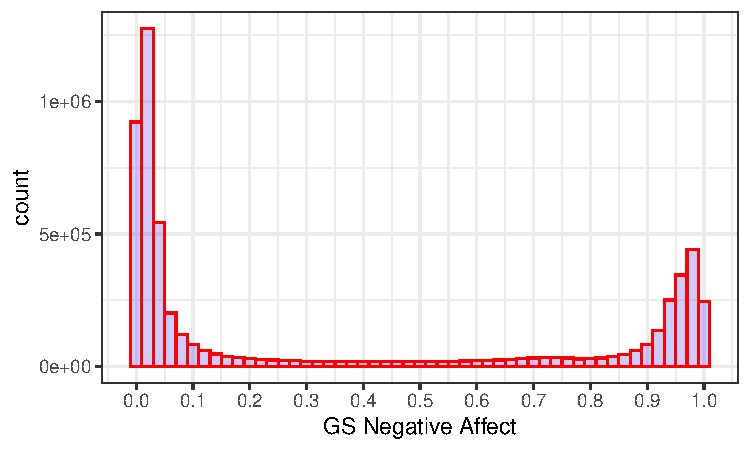
\includegraphics[width=0.48\linewidth]{plots/threshold_twitter_neg} }\subfloat[GS Positive Affect Twitter\label{fig:hist-plot-2}]{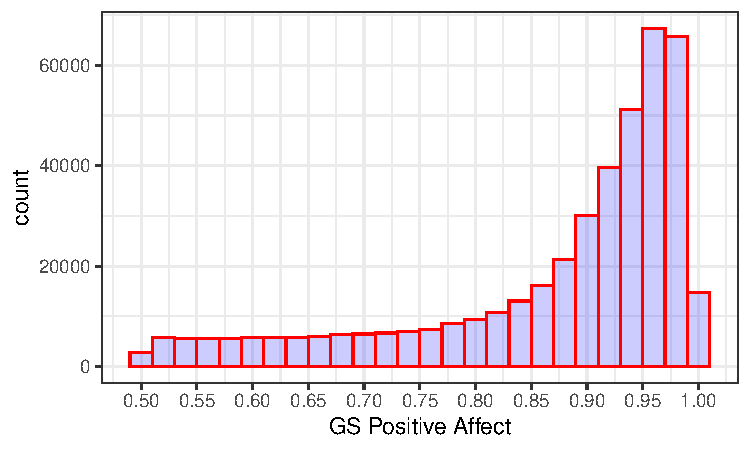
\includegraphics[width=0.48\linewidth]{plots/threshold_twitter_pos} }\newline\subfloat[GS Negative Affect Der Standard\label{fig:hist-plot-3}]{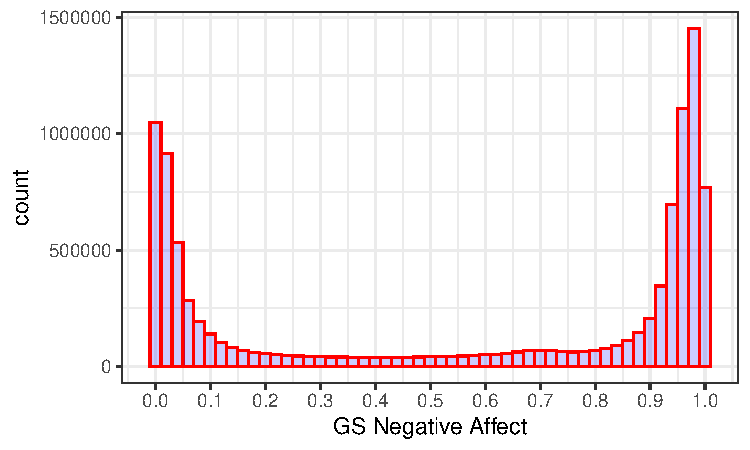
\includegraphics[width=0.48\linewidth]{plots/threshold_stand_neg} }\subfloat[GS Negative Affect Der Standard\label{fig:hist-plot-4}]{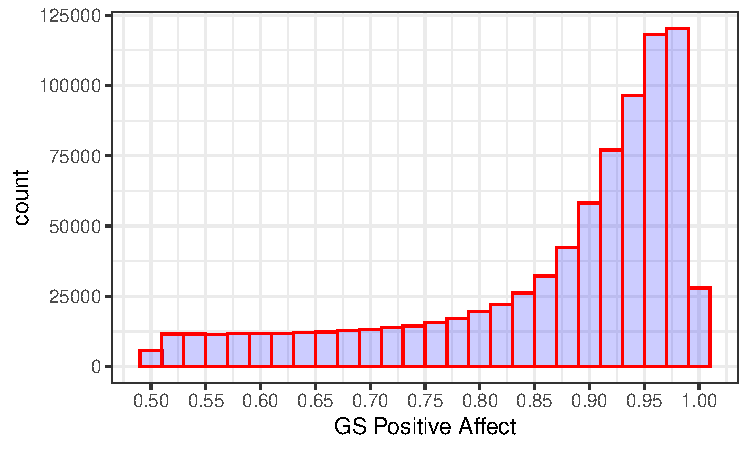
\includegraphics[width=0.48\linewidth]{plots/threshold_stand_pos} }

\textit{Note:} The histograms illustrate a visual aid to setting a threshold to categorize posts as negative or positive. In order to scale the plot in a way such that the decision to set the threshold at 0.9 can be understood the GS positive affect score distributions is only displayed for higher values, i.e., ranging from 0.5 to 1.
\end{figure*}

\begin{figure*}
\caption{Boxplots of Surveyed Anger, Anxiety and Depression \label{fig:survey-plot}}
\subfloat[Anger\label{fig:survey-plot-11}]{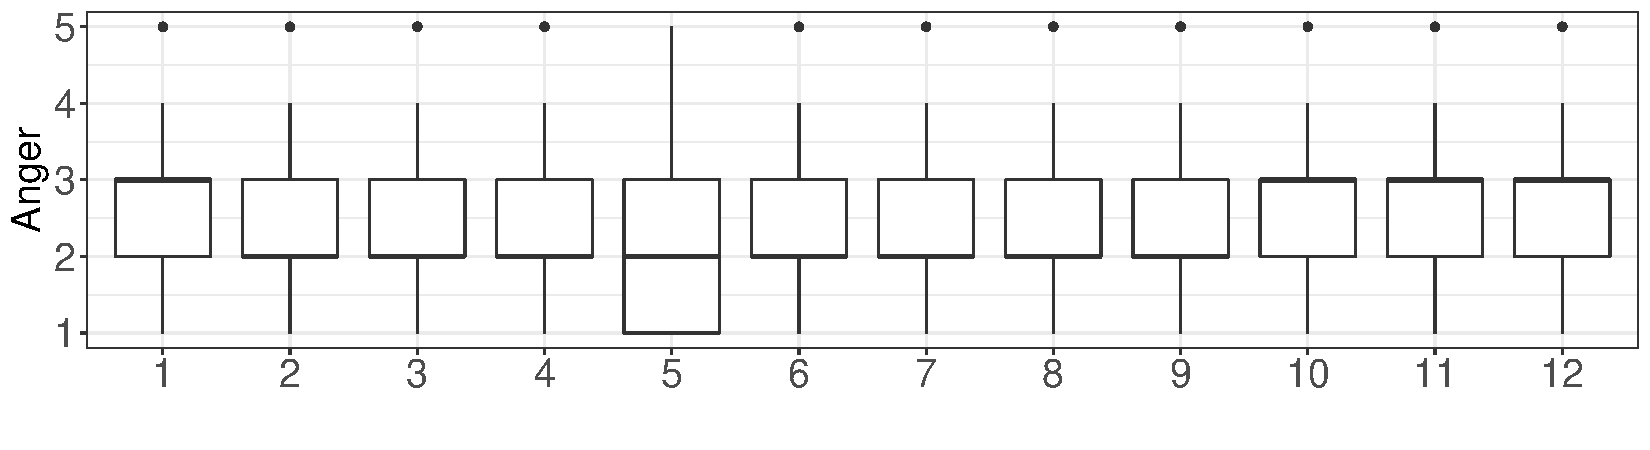
\includegraphics{plots/boxplot_ang} }\newline\subfloat[Anxiety\label{fig:survey-plot-12}]{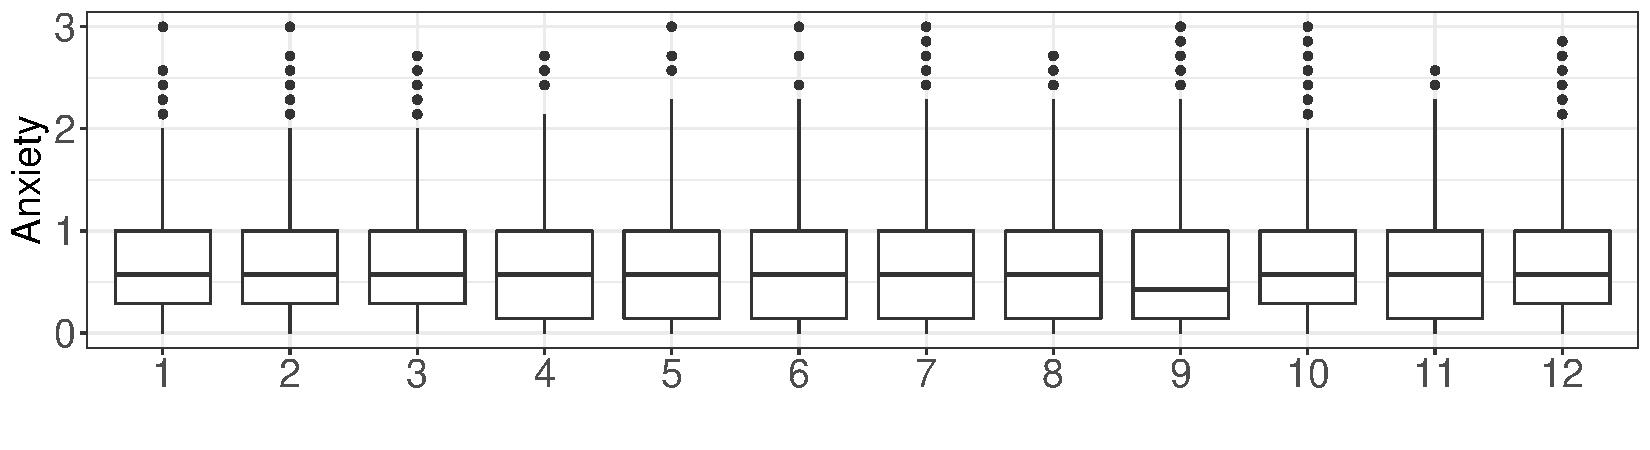
\includegraphics{plots/boxplot_anx} }\newline\subfloat[Depression\label{fig:survey-plot-13}]{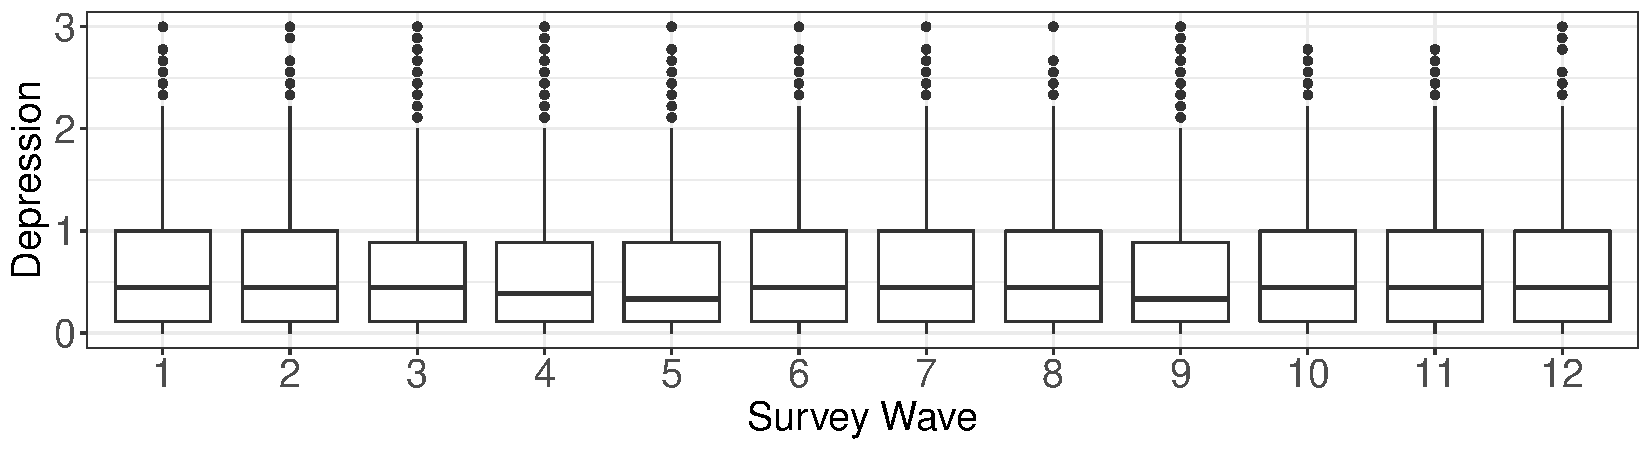
\includegraphics{plots/boxplot_dep} }
\end{figure*}

\begin{figure*}
\caption{Three-Day Rolling Means of Negative and Positive Emotionality and Affect in Twitter and Der Standard in 2020  \label{fig:survey-plot-3}}

\subfloat[Negative Affect\label{fig:survey-plot-1}]{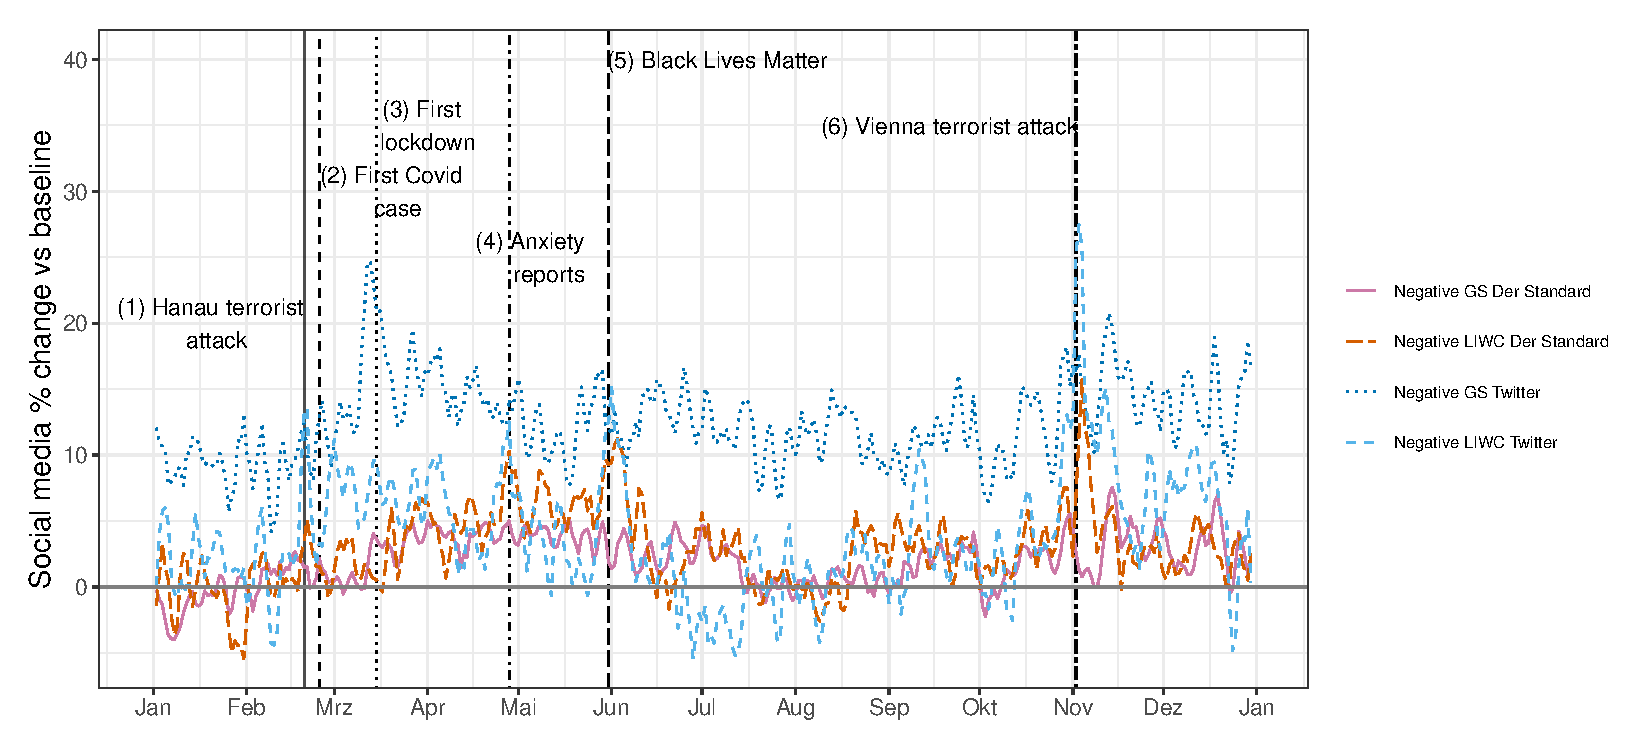
\includegraphics{plots/negative_affect_smooth} }\newline\subfloat[Positive Affect \label{fig:survey-plot-2}]{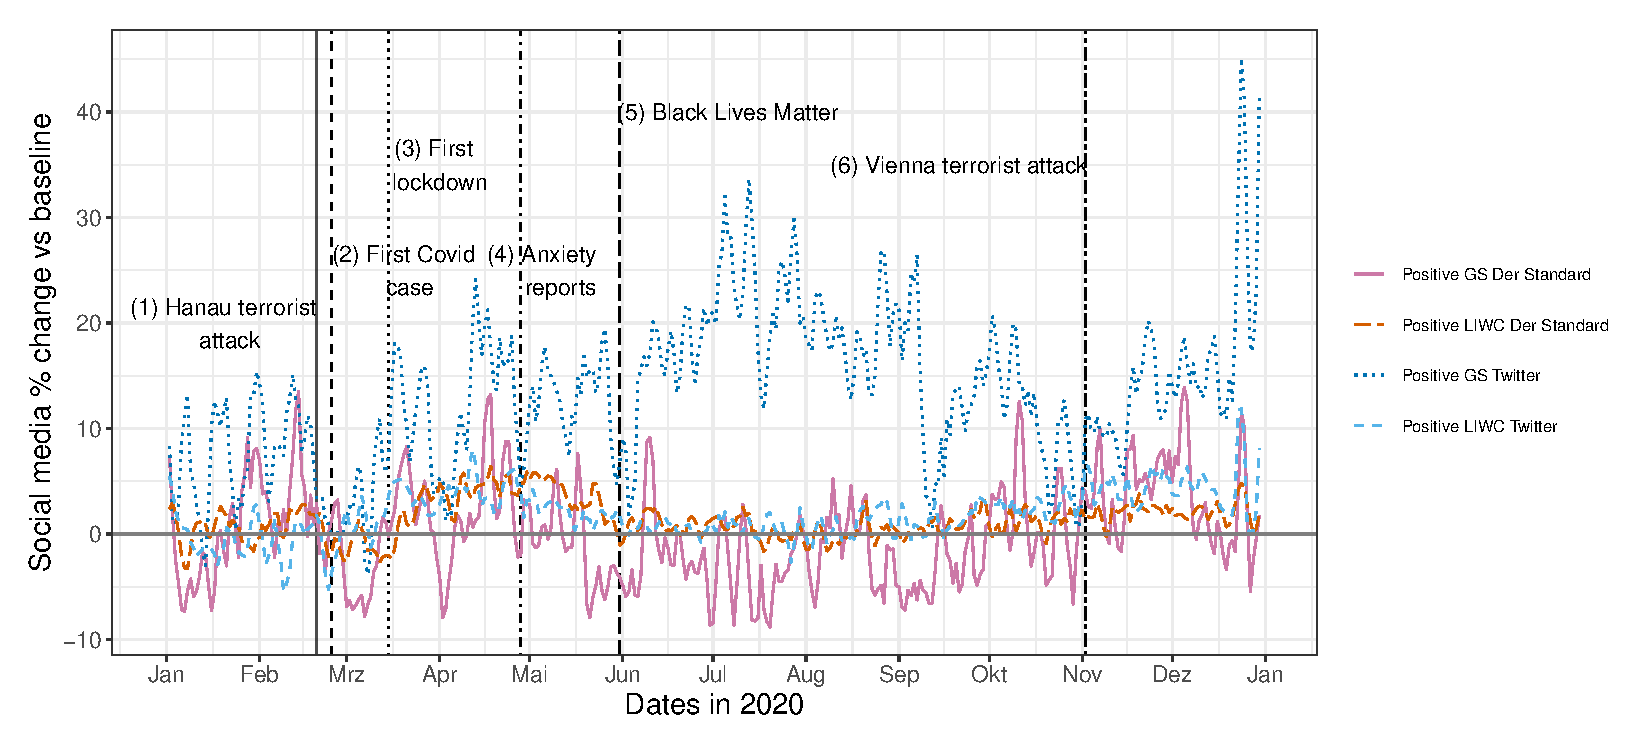
\includegraphics{plots/positive_affect_smooth}}

\textit{Note:} This plot pictures the three-day rolling means of the baseline-corrected LIWC and GS negative and positive emotionality and affect measures in Twitter. For a more detailed description of the events depicted by the vertical lines see Figure~\ref{fig:survey-plot-4}.   
\end{figure*}

\begin{table*}[tbp]

\begin{center}
\begin{threeparttable}

\caption{\label{tab:table-appendix-1}Spearman's Rank Correlations' Confidence Intervals Computed by Bootstrap and Analytical Procedure and its Value of Confidence for Twitter}

\small{

\begin{tabular}{lllllll}
\toprule
 & \multicolumn{1}{c}{Anx Surv Neg GS} & \multicolumn{1}{c}{Depr Surv Neg GS} & \multicolumn{1}{c}{Ang Surv Neg GS} & \multicolumn{1}{c}{Anx Surv Anx} & \multicolumn{1}{c}{Ang Surv Ang} & \multicolumn{1}{c}{Depr Surv Sad}\\
\midrule
Rho & 0.33 & 0.15 & 0.53 & 0.36 & -0.29 & 0.51\\
Confidence & 0.98 & 0.98 & 0.98 & 0.97 & 0.95 & 0.90\\
Lower adj Boot & -0.44 & -0.64 & -0.24 & -0.38 & -0.76 & -0.04\\
Upper adj Boot & 0.89 & 0.69 & 0.85 & 0.86 & 0.37 & 0.89\\
Lower adj Woods & -0.27 & -0.42 & -0.05 & -0.24 & -0.73 & -0.08\\
Upper adj Woods & 0.74 & 0.64 & 0.84 & 0.76 & 0.30 & 0.84\\
\bottomrule
\addlinespace
\end{tabular}

}

\begin{tablenotes}[para]
\normalsize{\textit{Note.} Woods describes the chosen analytical procedure to compute confidence intervals. Since the Holm-procedure adjusts p-values and therefore also confidence intervals, adjusted confidence intervals are listed in the table. Adjusted is abbreviated with adj. Ang, Anx, Depr, Surv are abbreviations for anger, anxiety, depression and survey.}
\end{tablenotes}

\end{threeparttable}
\end{center}

\end{table*}

\begin{table*}[tbp]

\begin{center}
\begin{threeparttable}

\caption{\label{tab:table-appendix-2}Spearman's Rank Correlations' Confidence Intervals Computed by Bootstrap and Analytical Procedure and its Value of Confidence for Der Standard}

\small{

\begin{tabular}{lllllll}
\toprule
 & \multicolumn{1}{c}{Anx Surv Neg GS} & \multicolumn{1}{c}{Depr Surv Neg GS} & \multicolumn{1}{c}{Ang Surv Neg GS} & \multicolumn{1}{c}{Anx Surv Anx} & \multicolumn{1}{c}{Ang Surv Ang} & \multicolumn{1}{c}{Depr Surv Sad}\\
\midrule
Rho & 0.13 & 0.13 & 0.39 & 0.37 & -0.17 & 0.48\\
Confidence & 0.98 & 0.98 & 0.98 & 0.97 & 0.95 & 0.90\\
Lower adj Boot & -0.64 & -0.61 & -0.33 & -0.34 & -0.65 & -0.06\\
Upper adj Boot & 0.87 & 0.78 & 0.88 & 0.85 & 0.44 & 0.87\\
Lower adj Woods & -0.45 & -0.45 & -0.21 & -0.23 & -0.65 & -0.12\\
Upper adj Woods & 0.62 & 0.62 & 0.78 & 0.77 & 0.41 & 0.82\\
\bottomrule
\addlinespace
\end{tabular}

}

\begin{tablenotes}[para]
\normalsize{\textit{Note.} Woods describes the chosen analytical procedure to compute confidence intervals. Since the Holm-procedure adjusts p-values and therefore also confidence intervals, adjusted confidence intervals are listed in the table. Adjusted is abbreviated with adj. Ang, Anx, Depr, Surv are abbreviations for anger, anxiety, depression and survey.}
\end{tablenotes}

\end{threeparttable}
\end{center}

\end{table*}

\begin{figure*}
\caption{Histogram and Q-Q Plot of Bootstrap Samples for Spearman's $\rho$ for Twitter \label{fig:survey-plot-7}}

\subfloat[Anger GS Negative\label{fig:survey-plot-7-1}]{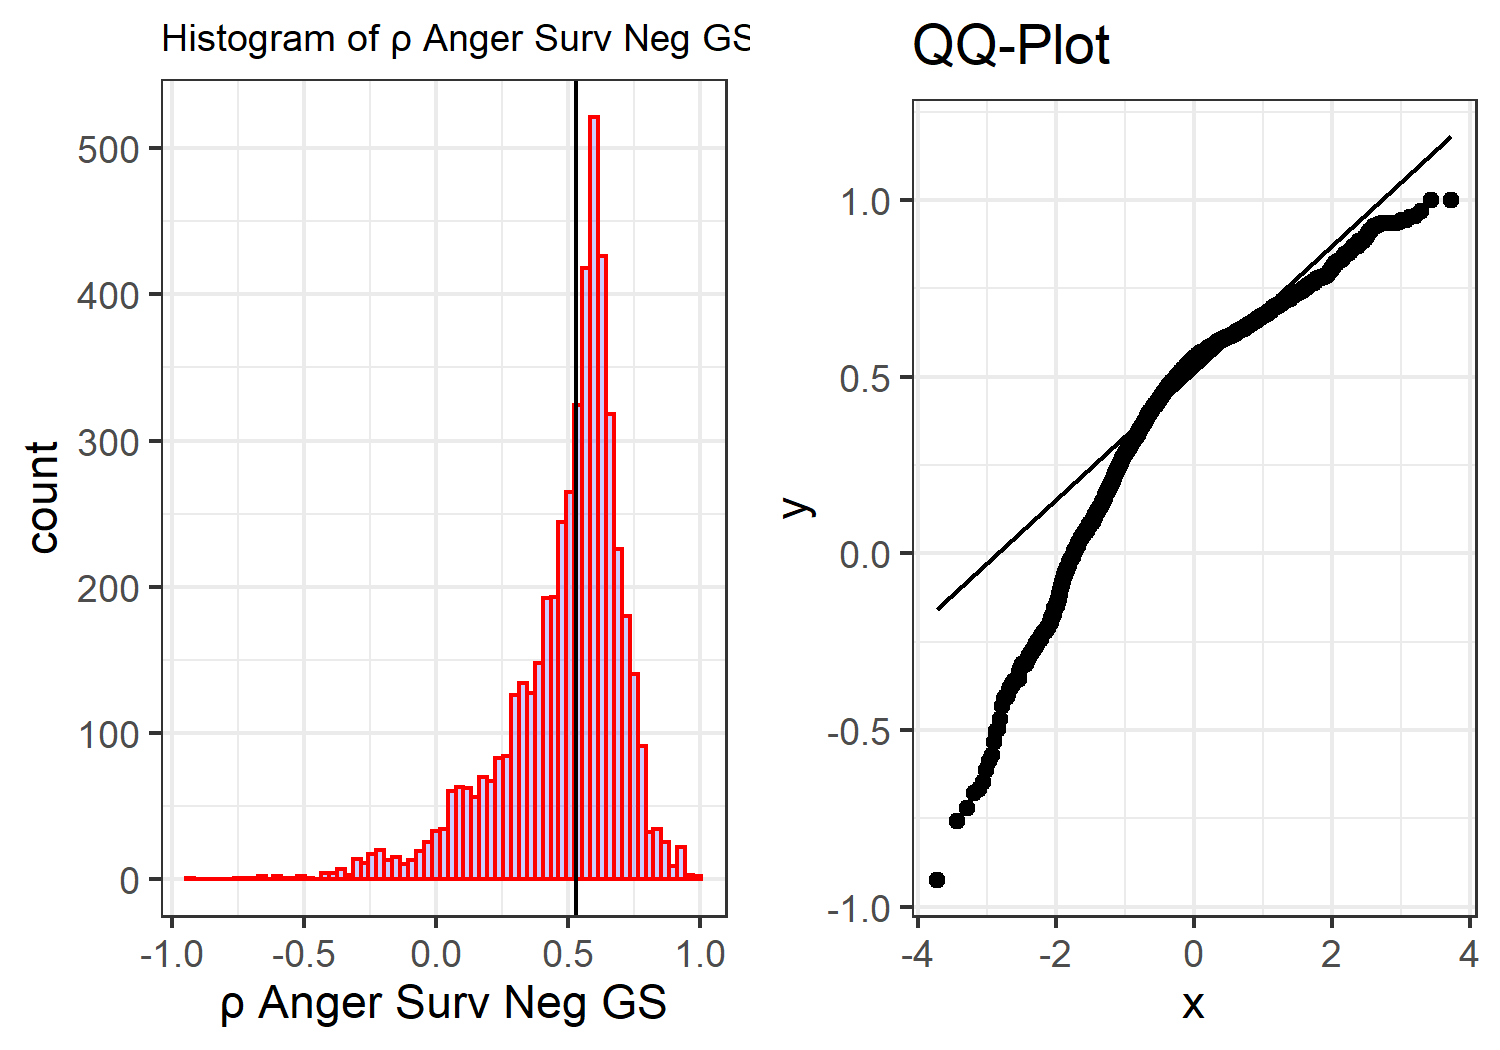
\includegraphics[width=0.48\linewidth]{plots/histboottwitter_ang_GS} }\subfloat[Anxiety GS Negative\label{fig:survey-plot-7-2}]{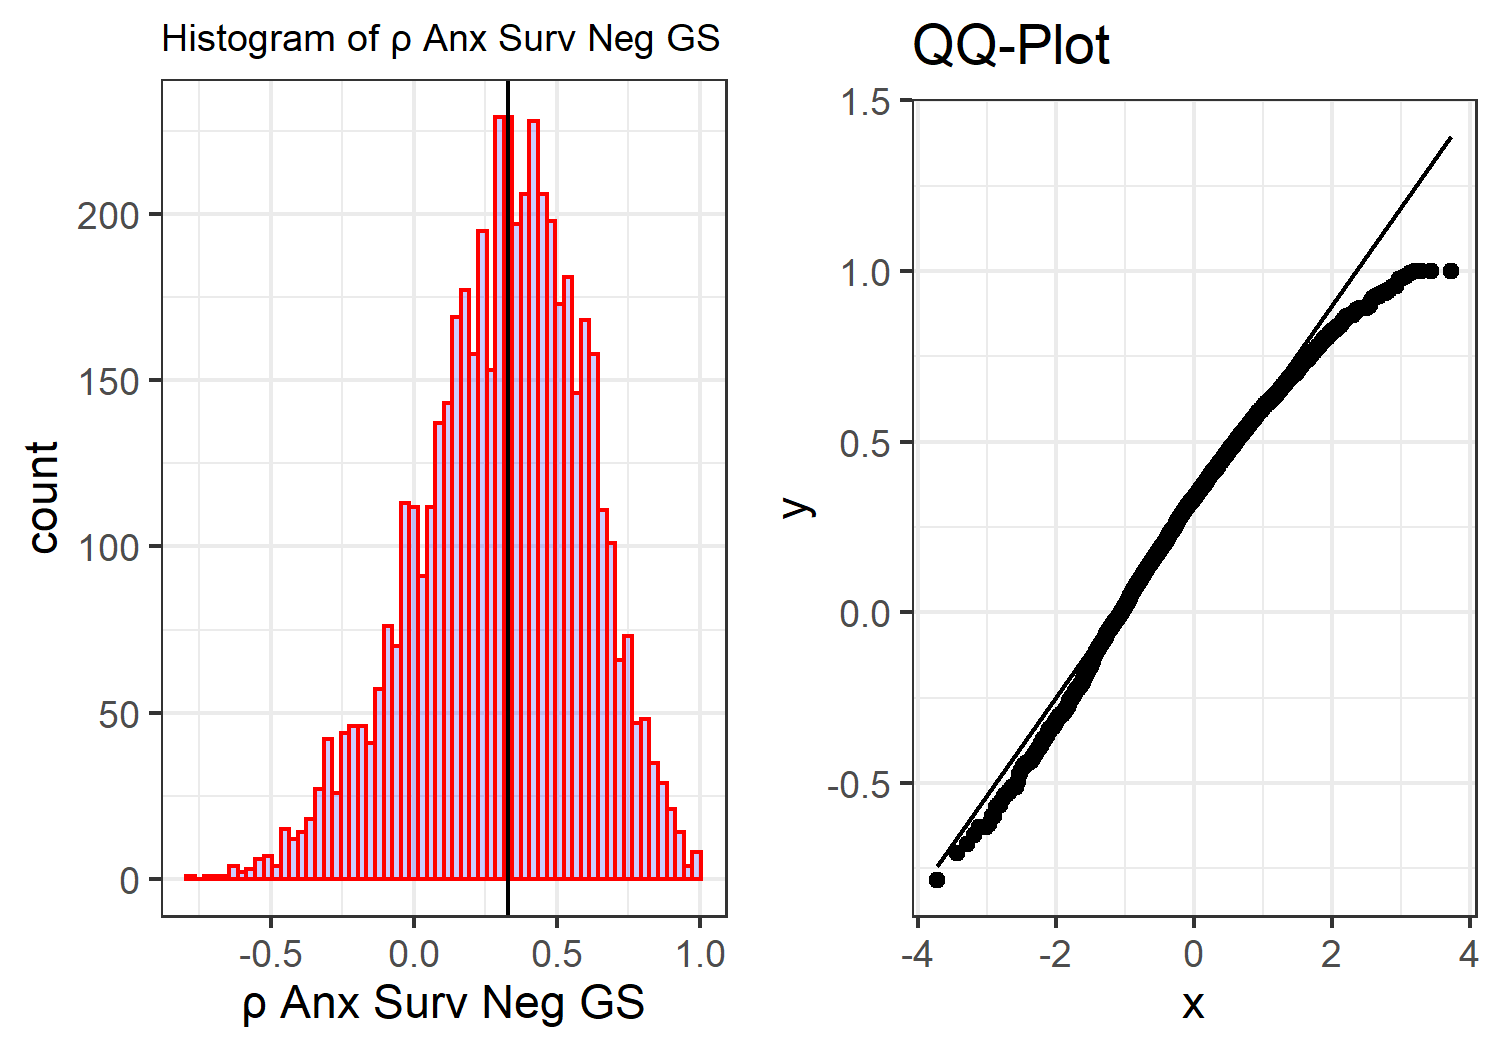
\includegraphics[width=0.48\linewidth]{plots/histboottwitter_anx_GS} }\newline\subfloat[Depression GS Negative\label{fig:survey-plot-7-3}]{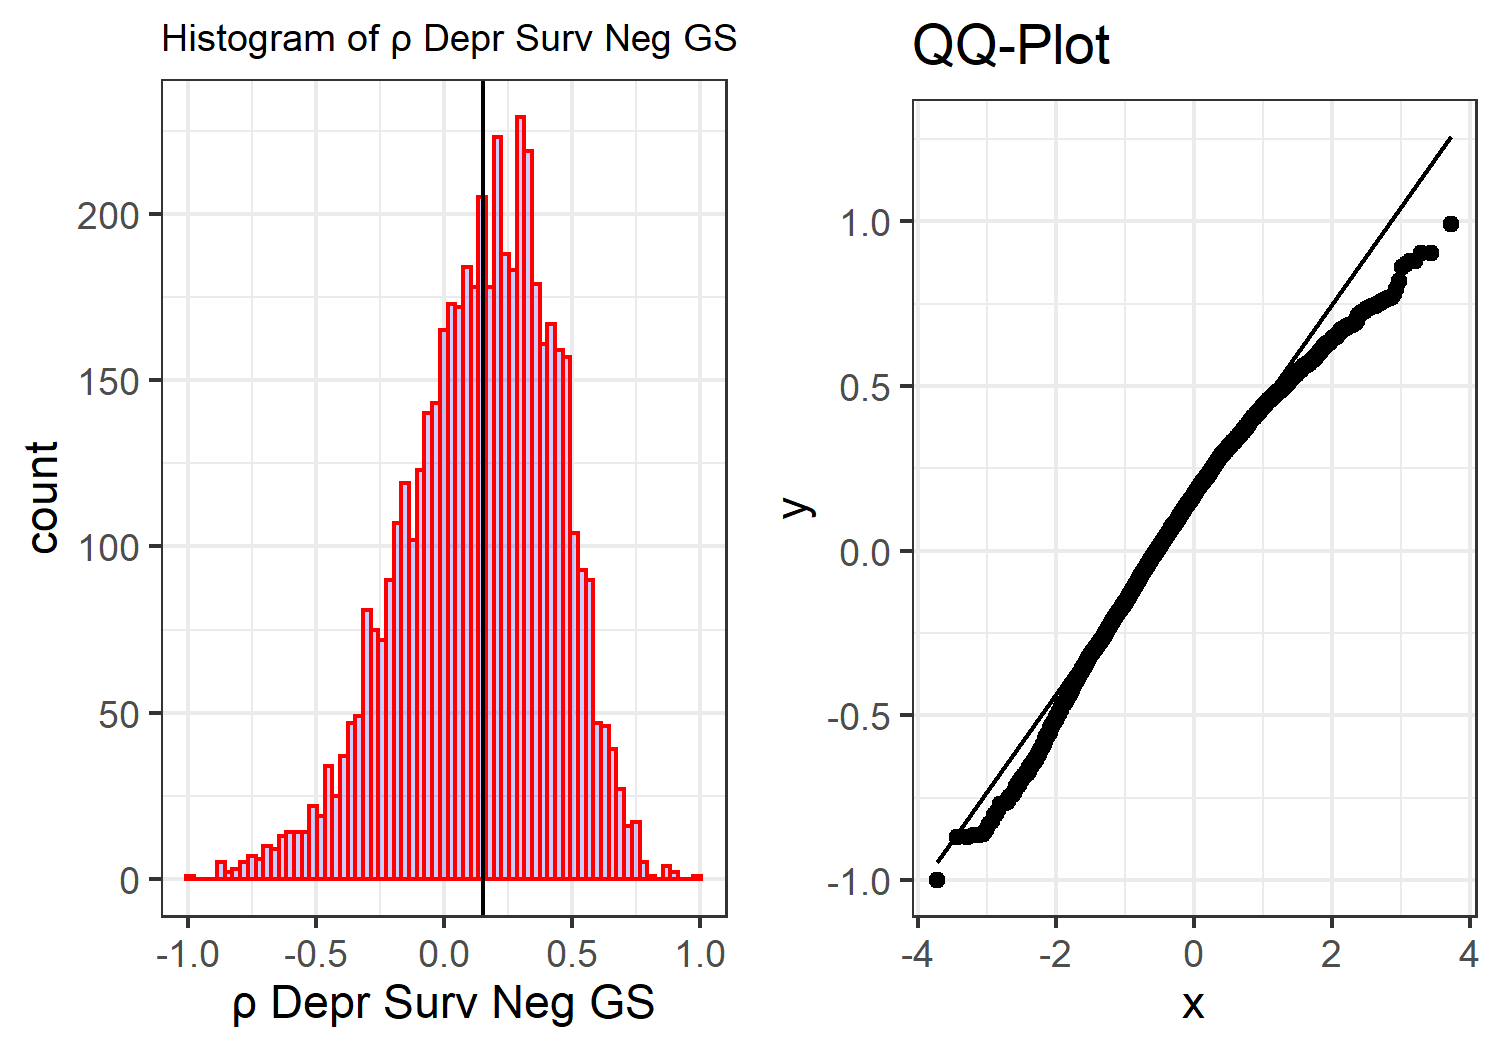
\includegraphics[width=0.48\linewidth]{plots/histboottwitter_depr_GS} }\subfloat[Anger LIWC Anger\label{fig:survey-plot-7-4}]{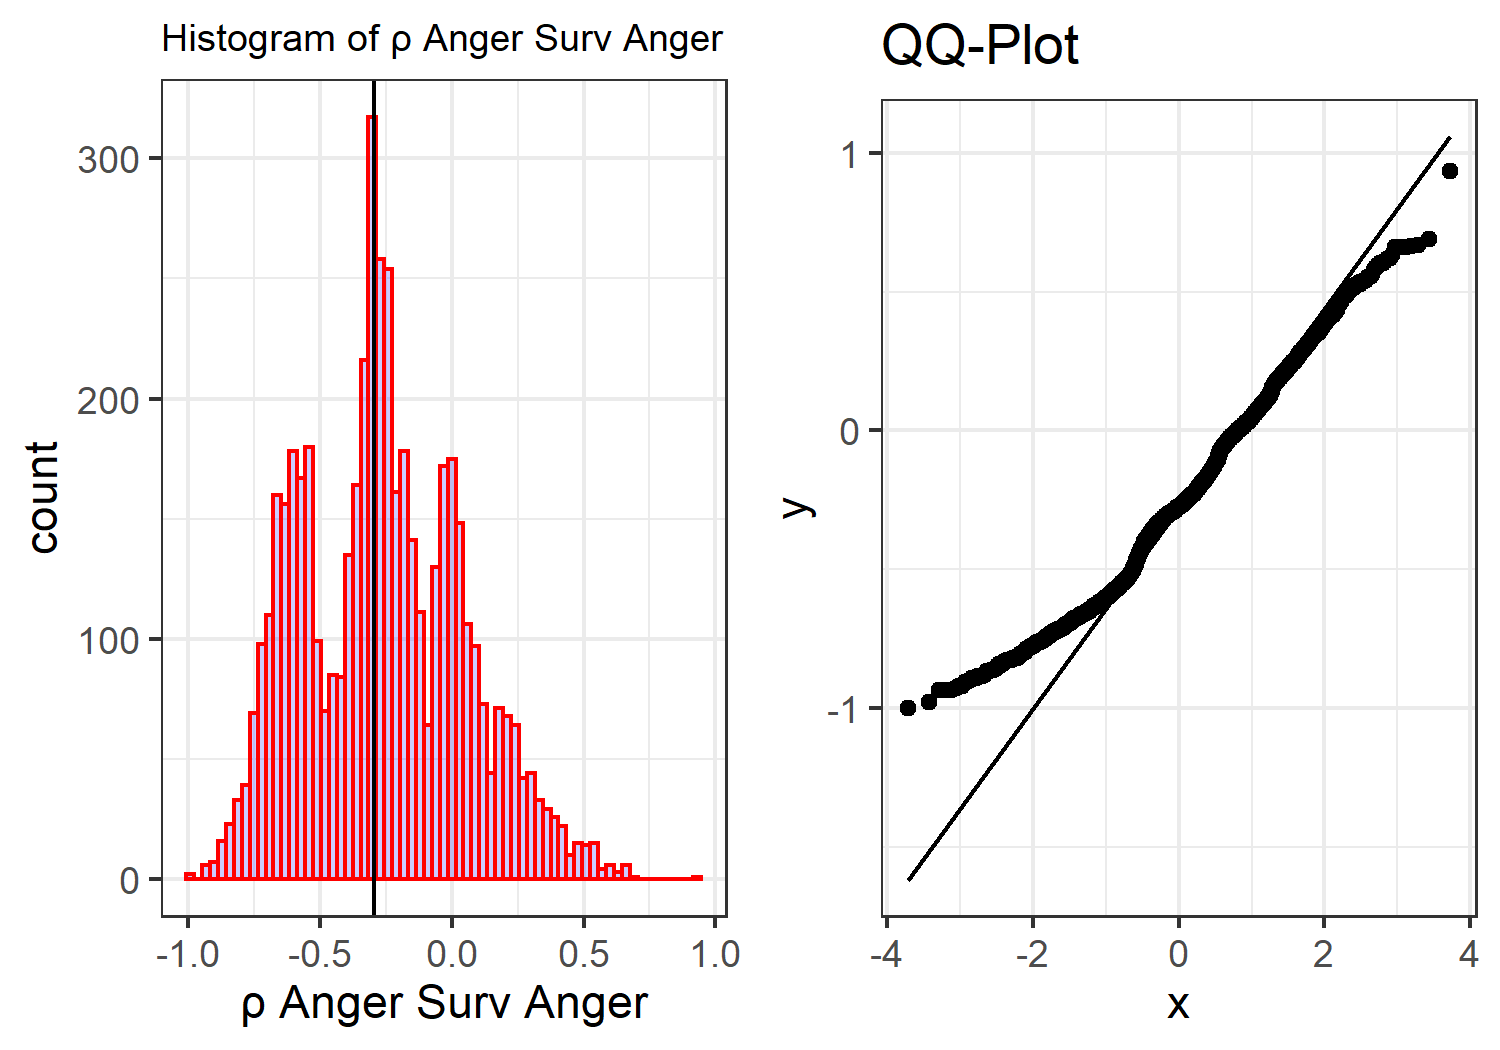
\includegraphics[width=0.48\linewidth]{plots/histboottwitter_ang_LIWC} }\newline\subfloat[Anxiety LIWC Anxiety\label{fig:survey-plot-7-5}]{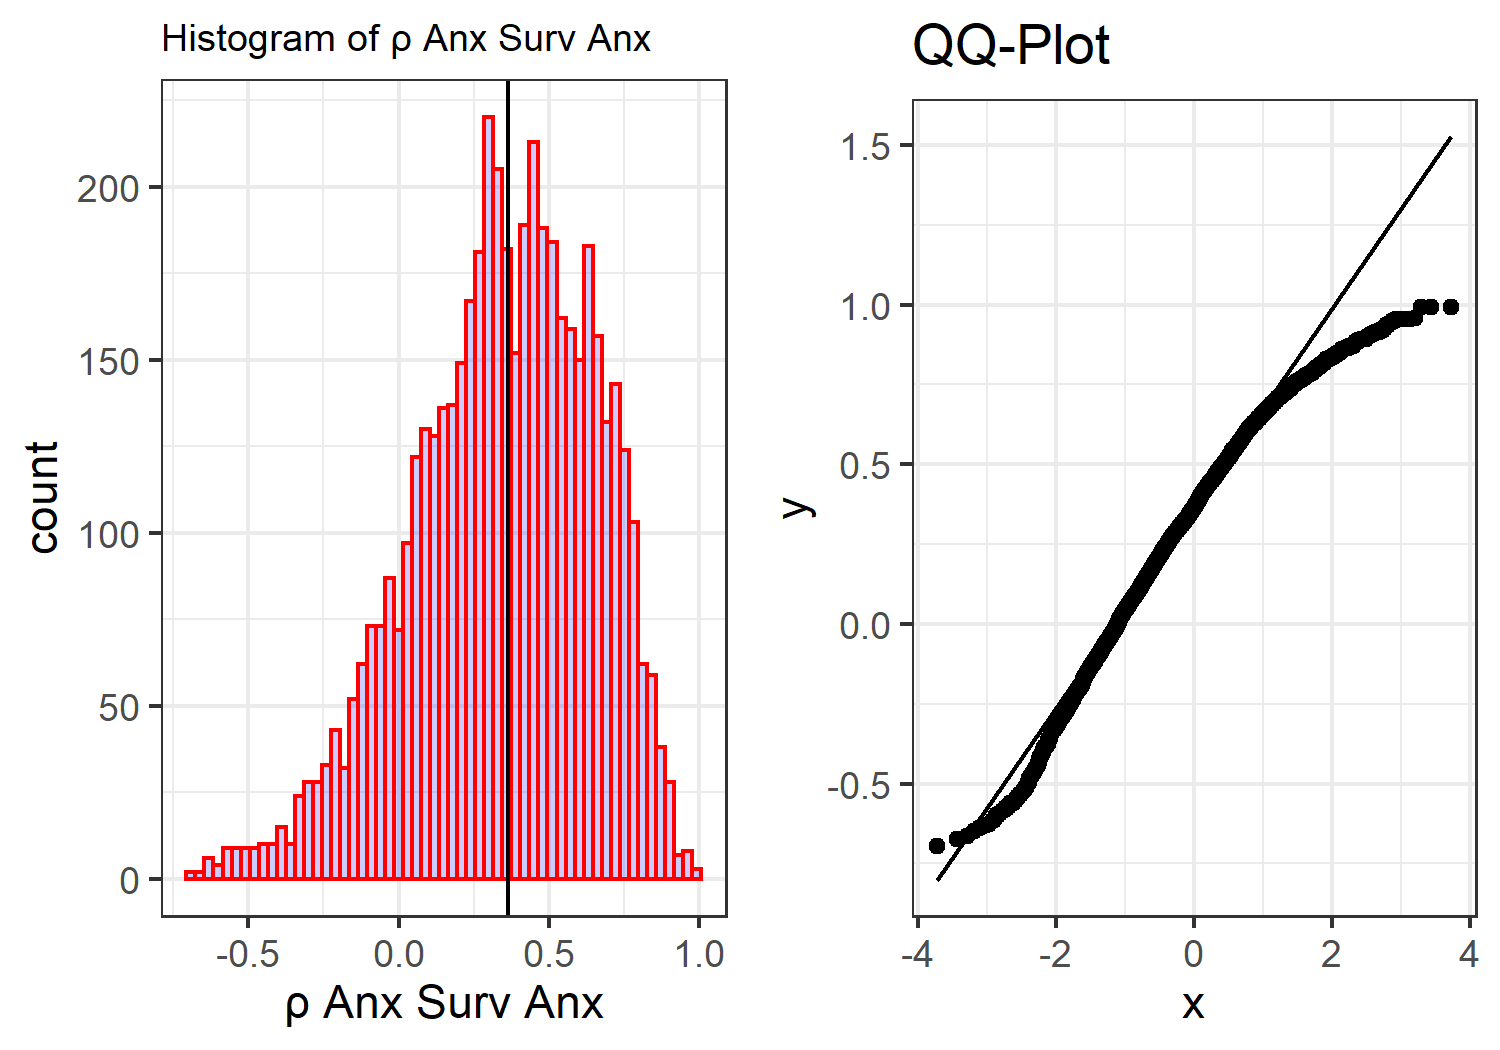
\includegraphics[width=0.48\linewidth]{plots/histboottwitter_anx_LIWC} }\subfloat[Depression LIWC Sadness\label{fig:survey-plot-7-6}]{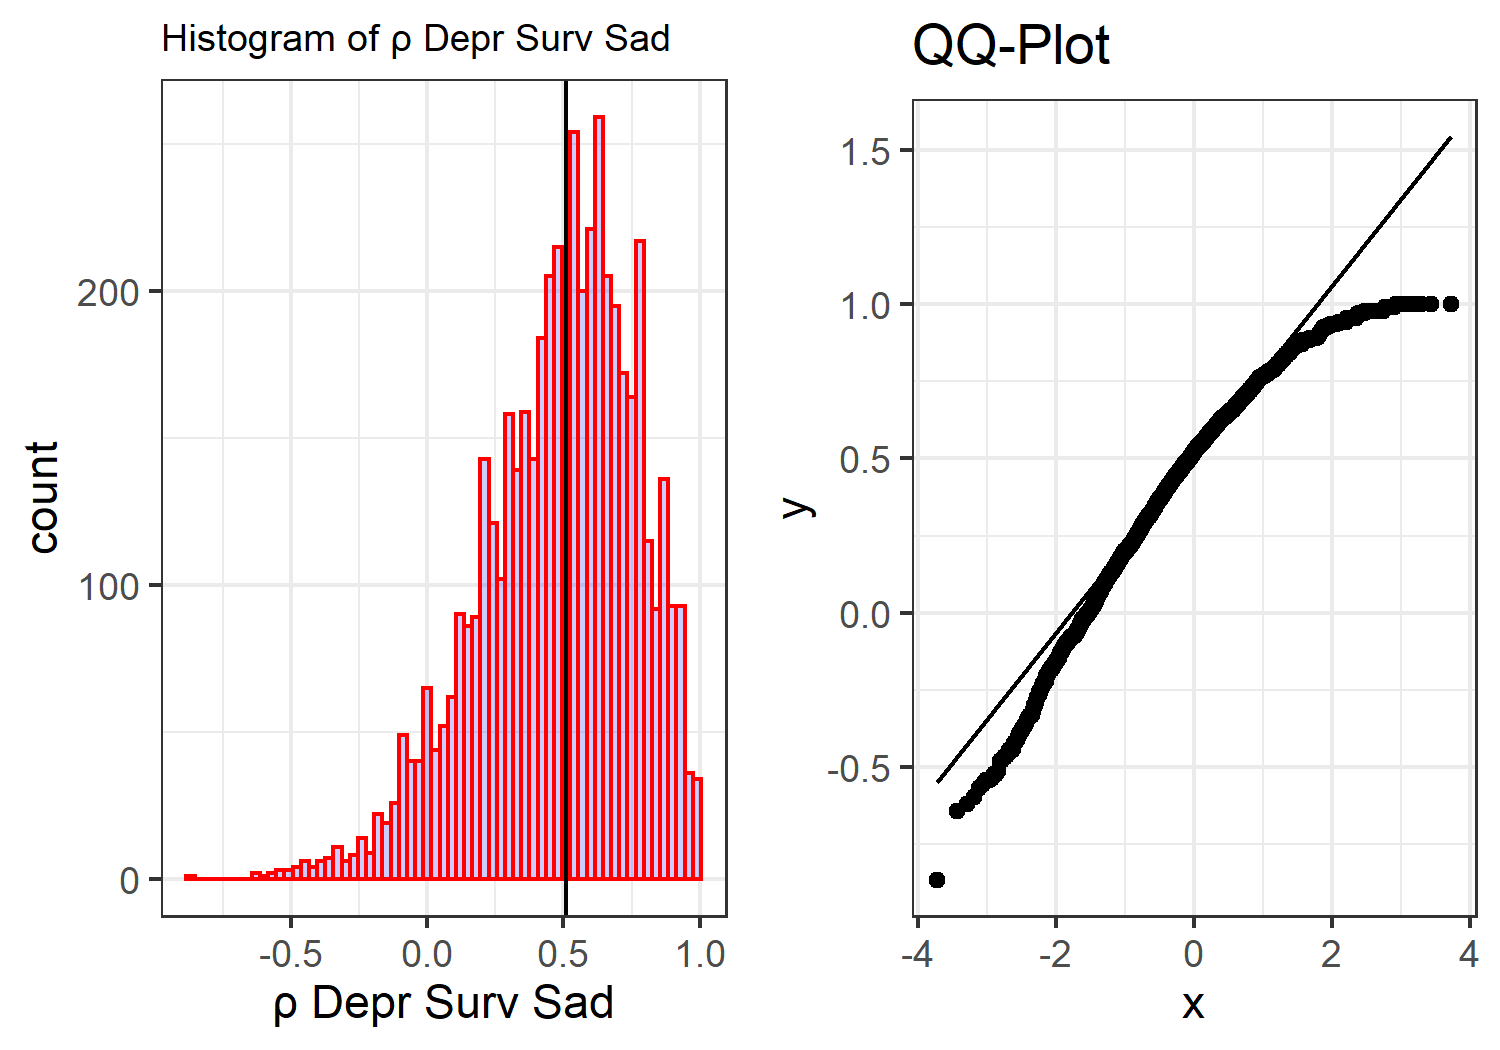
\includegraphics[width=0.48\linewidth]{plots/histboottwitter_depr_LIWC} }

\textit{Note:} Q-Q plots compare the empirical distribution's quantiles against - in this case - the quantile of a normal distribution. A larger deviance from the diagonal line therefore indicates that the normality assumption most analytical procedure presume is not met.

\end{figure*}

\begin{figure*}
\caption{Histogram and Q-Q Plot of Bootstrap Samples for Spearman's $\rho$ for Der Standard \label{fig:survey-plot-8}}

\subfloat[Anger GS Negative\label{fig:survey-plot-8-1}]{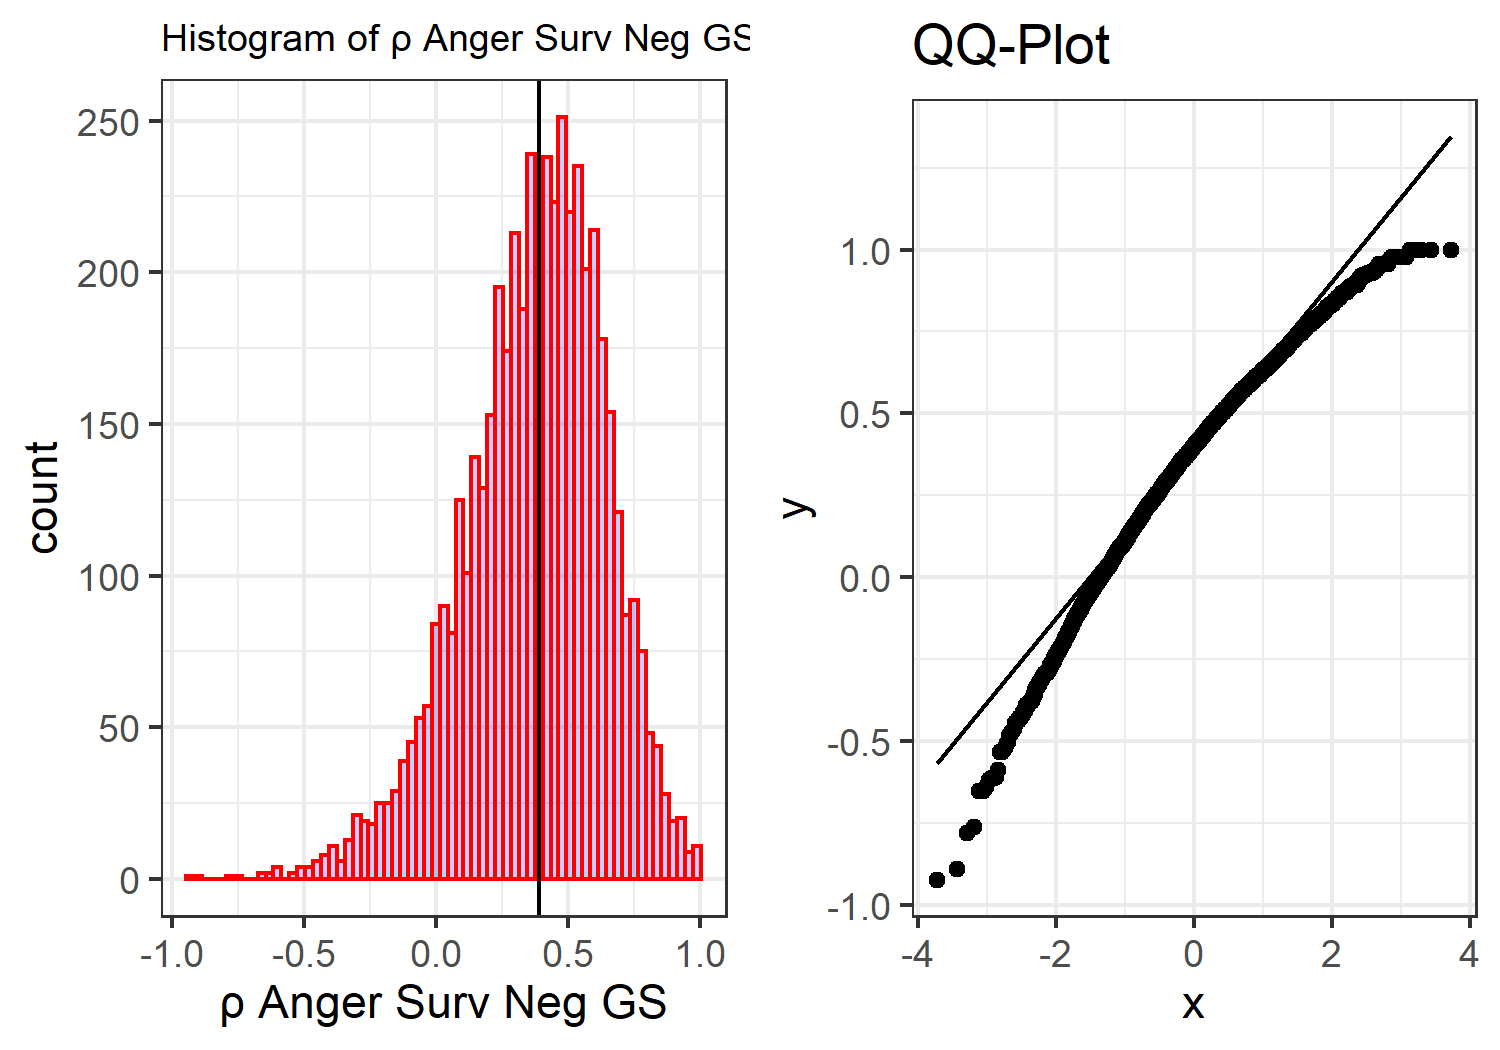
\includegraphics[width=0.48\linewidth]{plots/histbootstand_ang_GS} }\subfloat[Anxiety GS Negative\label{fig:survey-plot-8-2}]{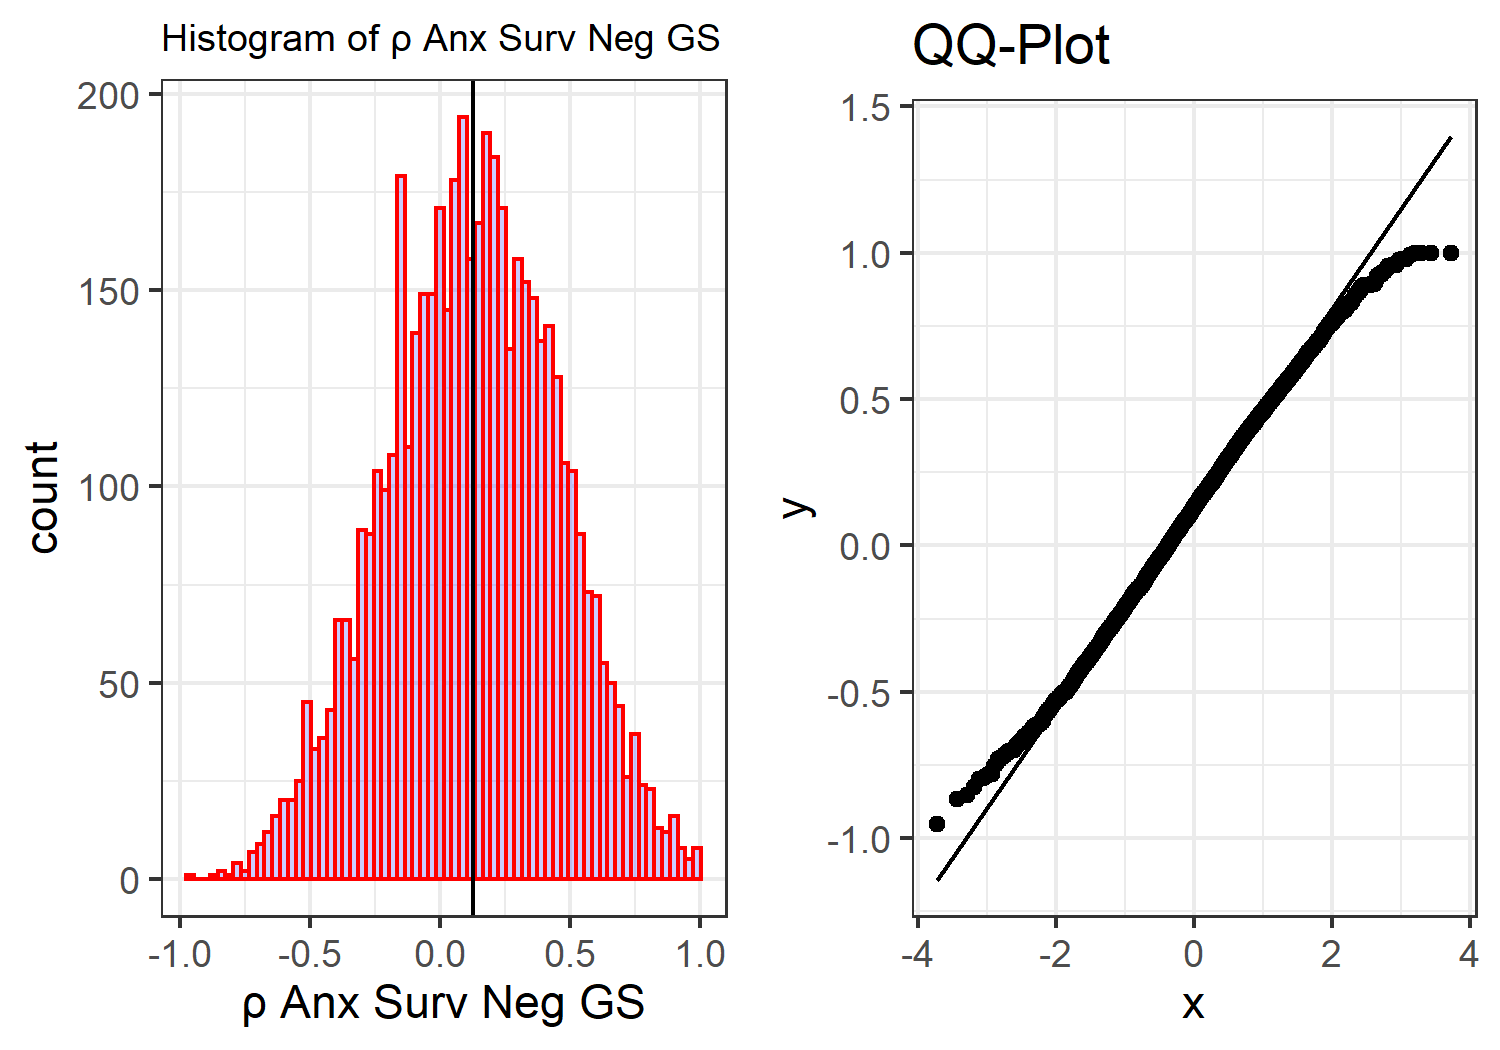
\includegraphics[width=0.48\linewidth]{plots/histbootstand_anx_GS} }\newline\subfloat[Depression GS Negative\label{fig:survey-plot-8-3}]{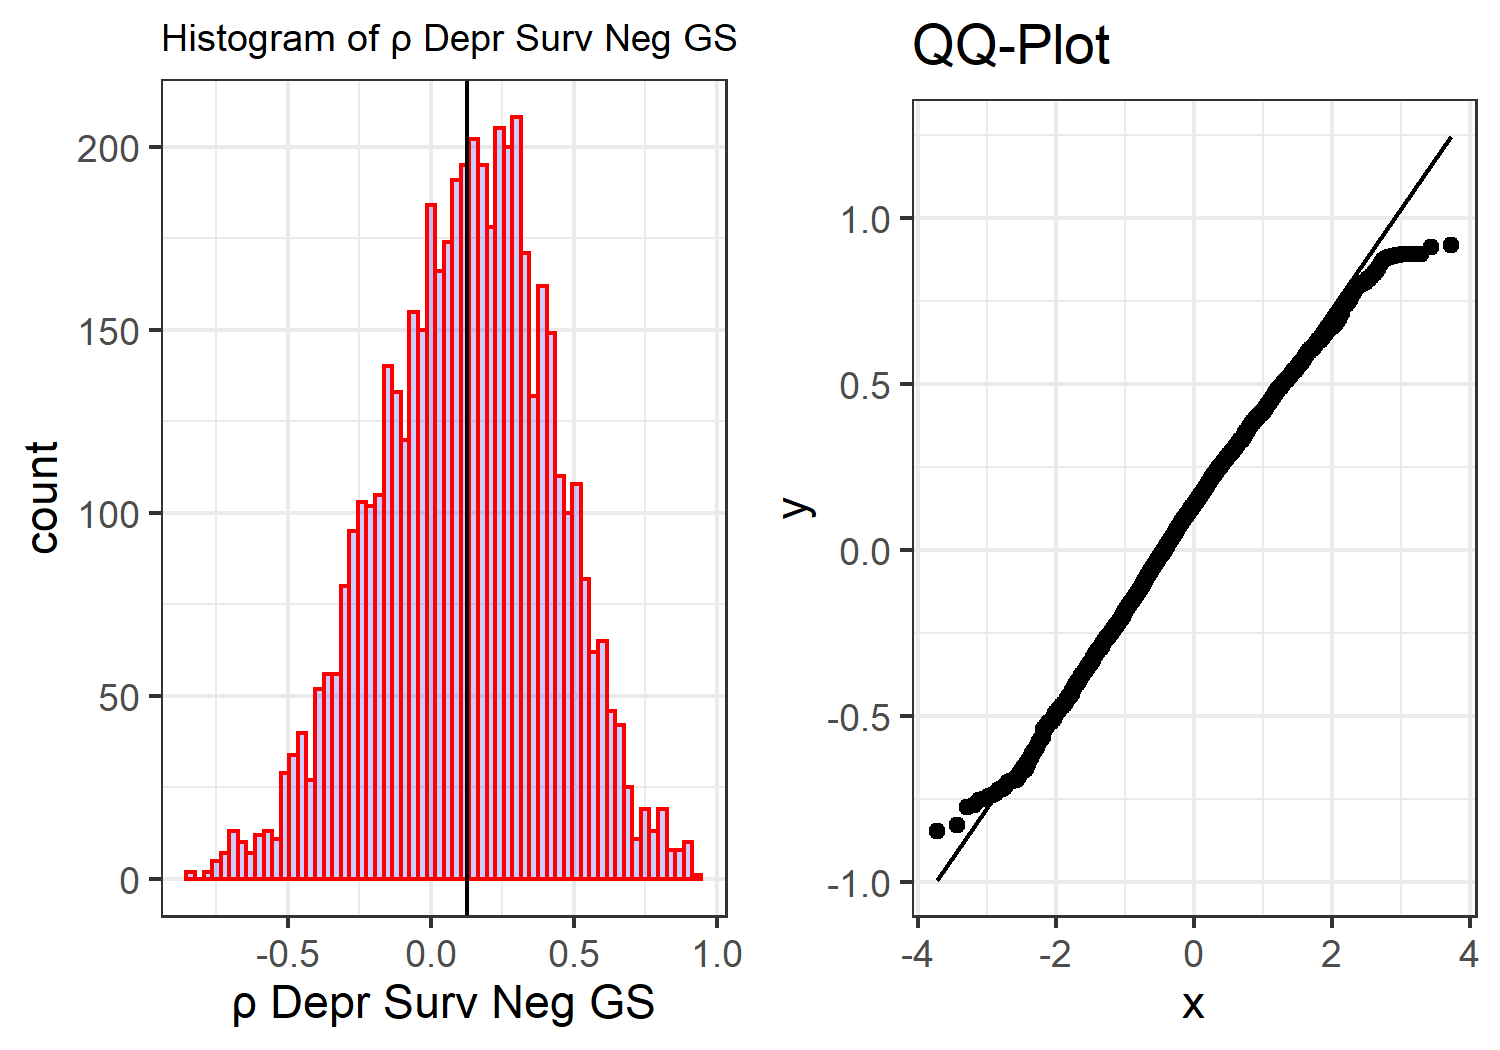
\includegraphics[width=0.48\linewidth]{plots/histbootstand_depr_GS} }\subfloat[Anger LIWC Anger\label{fig:survey-plot-8-4}]{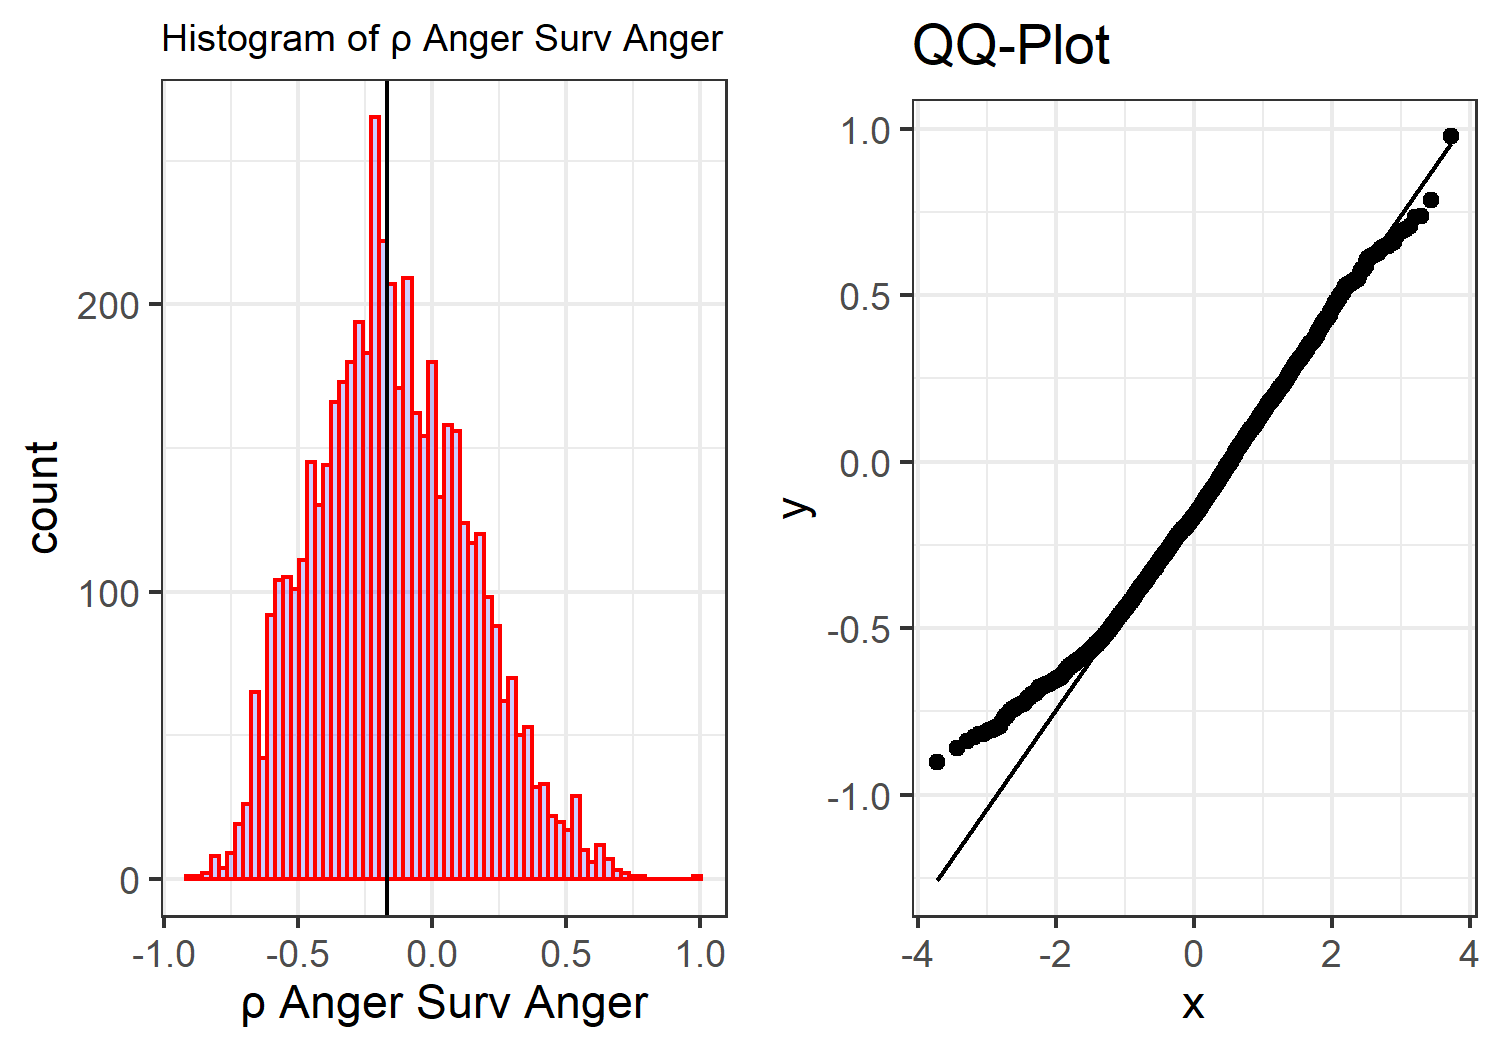
\includegraphics[width=0.48\linewidth]{plots/histbootstand_ang_LIWC} }\newline\subfloat[Anxiety LIWC Anxiety\label{fig:survey-plot-8-5}]{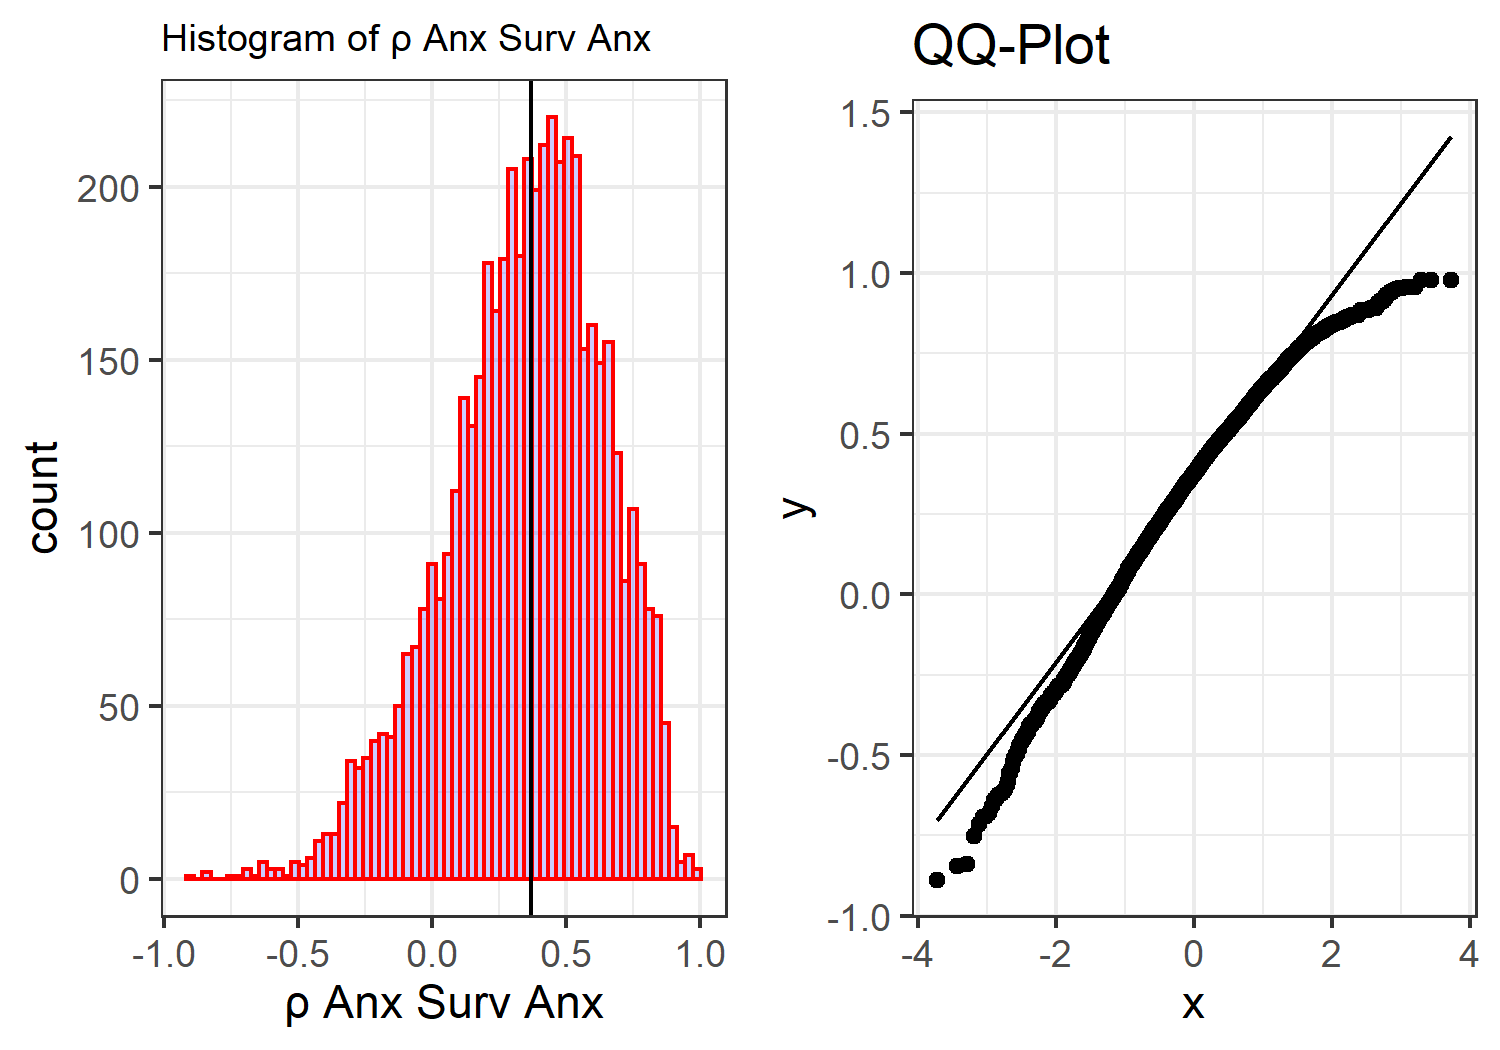
\includegraphics[width=0.48\linewidth]{plots/histbootstand_anx_LIWC} }\subfloat[Depression LIWC Sadness\label{fig:survey-plot-8-6}]{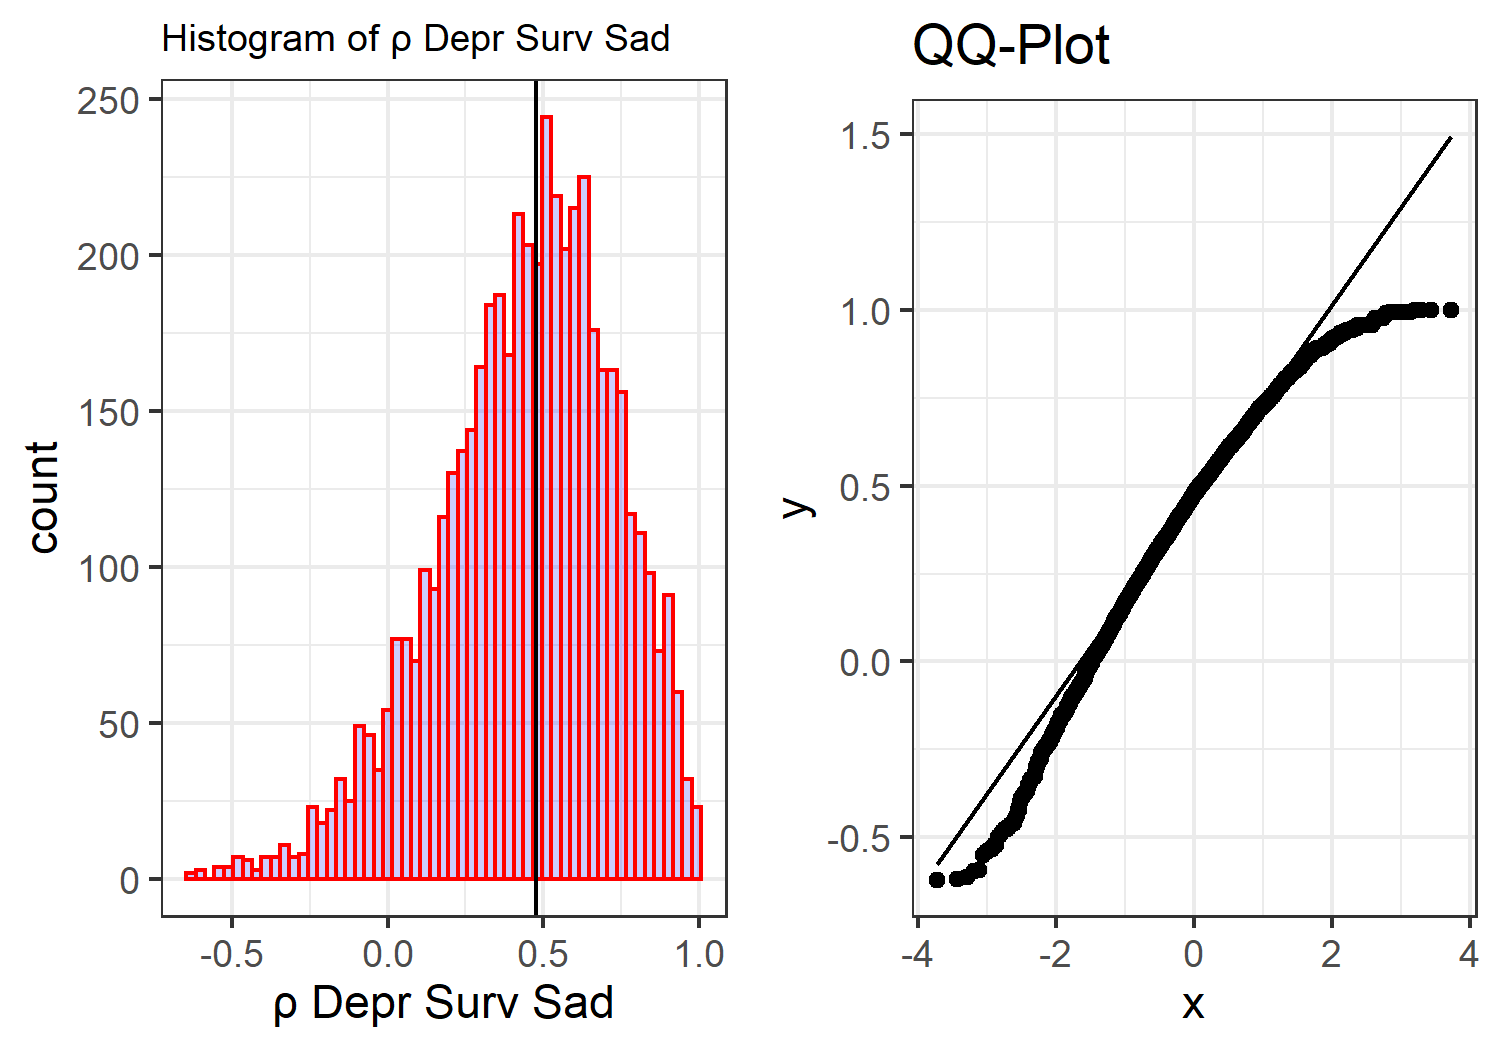
\includegraphics[width=0.48\linewidth]{plots/histbootstand_depr_LIWC} }

\end{figure*}

\begin{figure*}
\caption{Three-Day Rolling Means of LIWC Anxiety in Tweets from Users in Vienna and Upper Austria in 2020 Grouped by Gender}\label{fig:Anx-gender-region}
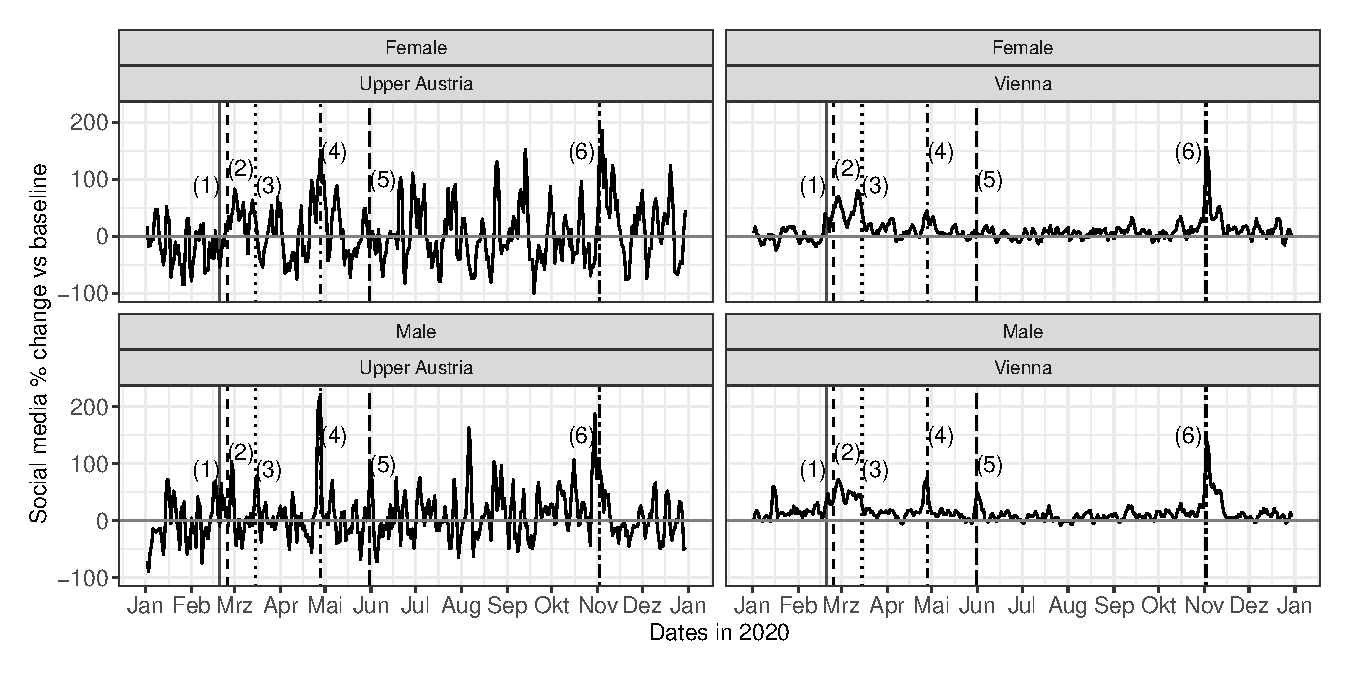
\includegraphics[width=\textwidth]{plots/plt_anxiety}

\textit{Note:} This plot pictures the three-day rolling means of the baseline-corrected LIWC anxiety measure in Twitter split by gender and two example federal states, Vienna and Upper Austria. The vertical lines portray important events stirring emotional responses in Austria: (1) the terrorist attack in Hanau, Germany on February 25, 2020, (2) the first Covid-19 case in Austria on February 25, 2020, (3) the first death from Covid-19 in Austria on March 12, 2020, (4) press releases about considerations of public agencies to stir anxiety of the population at the beginning of the pandemic on April 28, 2020, (5) Black Lives Matter demonstrations against police brutality on May 31, 2020, and (6) the terrorist attack in Vienna, Austria on November 02, 2020.  
\end{figure*}

\begin{figure*}
\caption{Three-Day Rolling Means of LIWC Sadness in Tweets from Users in Vienna and Upper Austria in 2020 Grouped by Gender}\label{fig:Sad-gender-region}
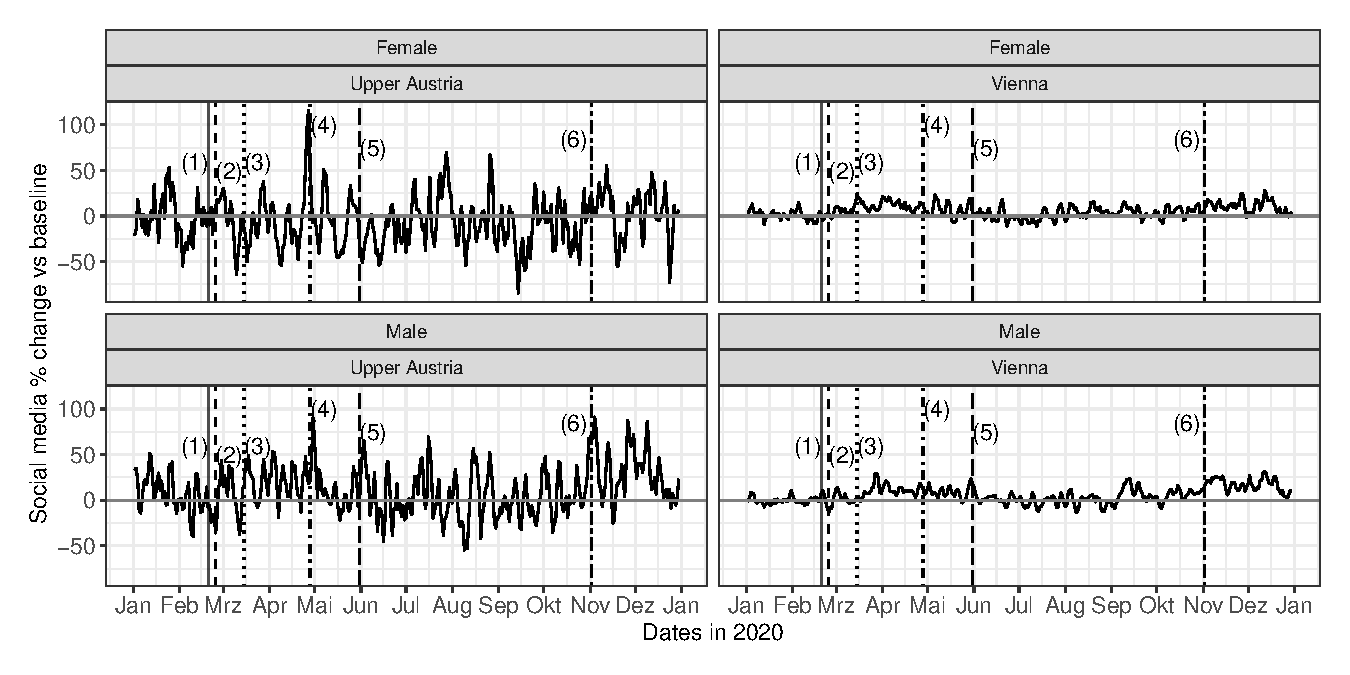
\includegraphics[width=\textwidth]{plots/plt_sadness}

\textit{Note:} This plot pictures the three-day rolling means of the baseline-corrected LIWC sadness measure in Twitter split by gender and two example federal states, Vienna and Upper Austria. The vertical lines portray important events stirring emotional responses in Austria: (1) the terrorist attack in Hanau, Germany on February 25, 2020, (2) the first Covid-19 case in Austria on February 25, 2020, (3) the first death from Covid-19 in Austria on March 12, 2020, (4) press releases about considerations of public agencies to stir anxiety of the population at the beginning of the pandemic on April 28, 2020, (5) Black Lives Matter demonstrations against police brutality on May 31, 2020, and (6) the terrorist attack in Vienna, Austria on November 02, 2020.
\end{figure*}

\begin{figure*}
\caption{Three-Day Rolling Means of GS Negative Affect in Tweets from Users in Vienna and Upper Austria in 2020 Grouped by Gender}\label{fig:GS-gender-region}
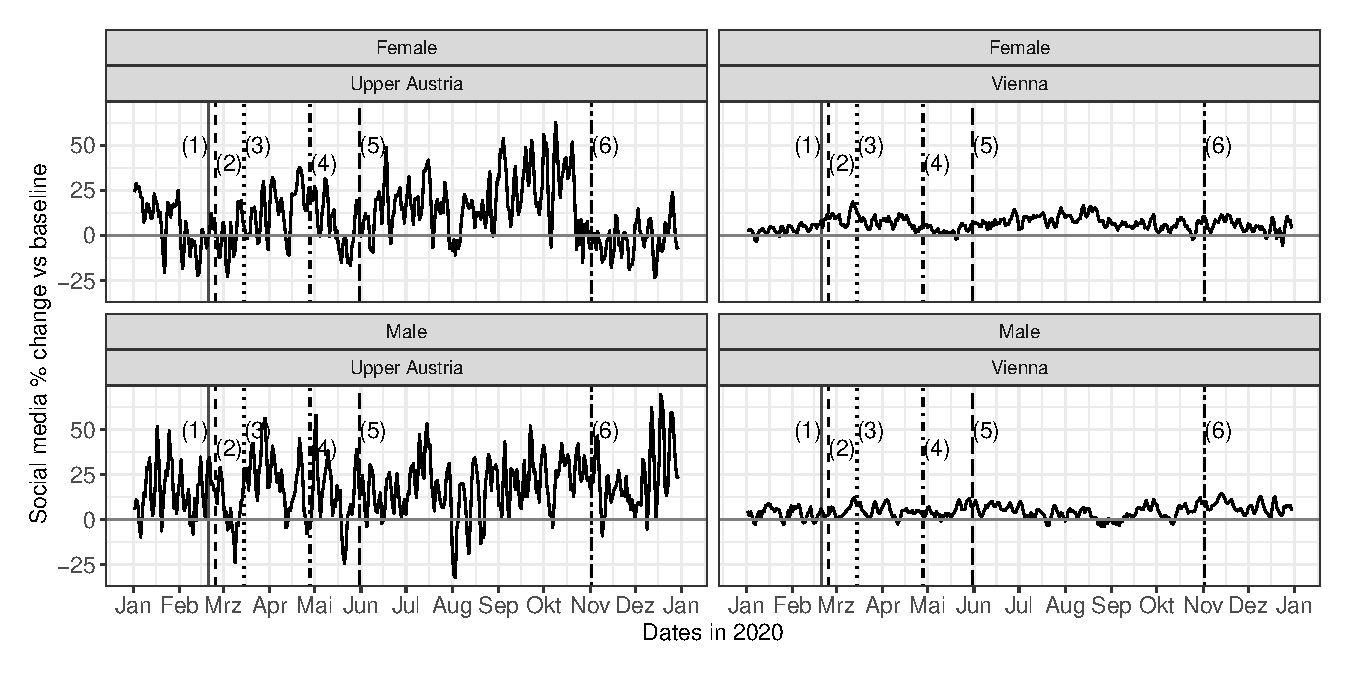
\includegraphics[width=\textwidth]{plots/plt_negGs} 

\textit{Note:} This plot pictures the three-day rolling means of the baseline-corrected GS negative affect measure in Twitter split by gender and two example federal states, Vienna and Upper Austria. The vertical lines portray important events stirring emotional responses in Austria: (1) the terrorist attack in Hanau, Germany on February 25, 2020, (2) the first Covid-19 case in Austria on February 25, 2020, (3) the first death from Covid-19 in Austria on March 12, 2020, (4) press releases about considerations of public agencies to stir anxiety of the population at the beginning of the pandemic on April 28, 2020, (5) Black Lives Matter demonstrations against police brutality on May 31, 2020, and (6) the terrorist attack in Vienna, Austria on November 02, 2020.
\end{figure*}

\begin{table*}[b]

\begin{center}
\begin{threeparttable}

\caption{\label{tab:table-ang-GS}Hierarchical Regression - Influence of Gender, Federal State and GS Negative Affect on Survey Anger}

\small{

\begin{tabular}{lll}
\toprule
 & \multicolumn{1}{c}{Baseline} & \multicolumn{1}{c}{GS Negative}\\
\midrule
Intercept & $2.66$ $[2.56$, $2.76]$ & $2.70$ $[2.58$, $2.81]$\\
Male & $-0.24$ $[-0.32$, $-0.16]$ & $-0.26$ $[-0.34$, $-0.17]$\\
Salzburg & $0.12$ $[-0.01$, $0.24]$ & $0.16$ $[0.01$, $0.30]$\\
Styria & $-0.12$ $[-0.25$, $0.01]$ & $-0.13$ $[-0.26$, $-0.01]$\\
Tyrol & $-0.02$ $[-0.15$, $0.10]$ & $-0.08$ $[-0.23$, $0.08]$\\
Vienna & $-0.07$ $[-0.19$, $0.06]$ & $-0.08$ $[-0.21$, $0.04]$\\
GS Negative &  & $-0.18$ $[-0.49$, $0.13]$\\
$R^2$ [90\% CI] & $.31$ $[0.17$, $0.41]$ & $.32$ $[0.17$, $0.41]$\\
$F$ & 10.46 & 8.97\\
$df_1$ & 5 & 6\\
$df_2$ & 114 & 113\\
$p$ & < .001 & < .001\\
$\mathrm{AIC}$ & -15.78 & -15.21\\
$\mathrm{BIC}$ & 3.73 & 7.09\\
$\Delta R^2$ [90\% CI] &  & $.01$ $[.00$, $.06]$\\
$F$ &  & 1.35\\
$df_1$ &  & 1\\
$df_2$ &  & 113\\
$p$ &  & .247\\
$\Delta \mathrm{AIC}$ &  & 0.57\\
$\Delta \mathrm{BIC}$ &  & 3.36\\
\bottomrule
\addlinespace
\end{tabular}

}

\begin{tablenotes}[para]
\normalsize{\textit{Note.} The baseline model refers to a model that only contains the demographic information, i.e., gender and federal state, as regressors. The second column refers to a second model that adds a sentiment measure to the regressors.}
\end{tablenotes}

\end{threeparttable}
\end{center}

\end{table*}

\begin{table*}[b]

\begin{center}
\begin{threeparttable}

\caption{\label{tab:table-anx-GS}Hierarchical Regression - Influence of Gender, Federal State and GS Negative Affect on Survey Anxiety}

\small{

\begin{tabular}{lll}
\toprule
 & \multicolumn{1}{c}{Baseline} & \multicolumn{1}{c}{GS Negative}\\
\midrule
Intercept & $0.76$ $[0.71$, $0.80]$ & $0.76$ $[0.72$, $0.81]$\\
Male & $-0.12$ $[-0.15$, $-0.08]$ & $-0.12$ $[-0.15$, $-0.08]$\\
Salzburg & $0.08$ $[0.02$, $0.13]$ & $0.09$ $[0.03$, $0.15]$\\
Styria & $0.01$ $[-0.05$, $0.06]$ & $0.00$ $[-0.05$, $0.06]$\\
Tyrol & $0.04$ $[-0.01$, $0.10]$ & $0.03$ $[-0.03$, $0.10]$\\
Vienna & $-0.04$ $[-0.09$, $0.01]$ & $-0.04$ $[-0.10$, $0.01]$\\
GS Negative &  & $-0.04$ $[-0.17$, $0.09]$\\
$R^2$ [90\% CI] & $.38$ $[0.23$, $0.47]$ & $.38$ $[0.23$, $0.47]$\\
$F$ & 13.73 & 11.45\\
$df_1$ & 5 & 6\\
$df_2$ & 114 & 113\\
$p$ & < .001 & < .001\\
$\mathrm{AIC}$ & -223.06 & -221.51\\
$\mathrm{BIC}$ & -203.54 & -199.21\\
$\Delta R^2$ [90\% CI] &  & $\Delta R^2 < .01$ $[.00$, $.03]$\\
$F$ &  & 0.43\\
$df_1$ &  & 1\\
$df_2$ &  & 113\\
$p$ &  & .513\\
$\Delta \mathrm{AIC}$ &  & 1.54\\
$\Delta \mathrm{BIC}$ &  & 4.33\\
\bottomrule
\end{tabular}

}

\end{threeparttable}
\end{center}

\end{table*}

\begin{table*}[tbp]

\begin{center}
\begin{threeparttable}

\caption{\label{tab:table-depr-GS}Hierarchical Regression - Influence of Gender, Federal State and GS Negative Affect on Survey Depression}

\small{

\begin{tabular}{lll}
\toprule
 & \multicolumn{1}{c}{Baseline} & \multicolumn{1}{c}{GS Negative}\\
\midrule
Intercept & $0.69$ $[0.65$, $0.73]$ & $0.73$ $[0.68$, $0.77]$\\
Male & $-0.14$ $[-0.18$, $-0.11]$ & $-0.15$ $[-0.19$, $-0.12]$\\
Salzburg & $0.07$ $[0.02$, $0.13]$ & $0.11$ $[0.05$, $0.17]$\\
Styria & $0.03$ $[-0.03$, $0.08]$ & $0.01$ $[-0.04$, $0.07]$\\
Tyrol & $0.03$ $[-0.02$, $0.08]$ & $-0.02$ $[-0.08$, $0.04]$\\
Vienna & $-0.02$ $[-0.07$, $0.03]$ & $-0.04$ $[-0.09$, $0.01]$\\
GS Negative &  & $-0.17$ $[-0.30$, $-0.04]$\\
$R^2$ [90\% CI] & $.42$ $[0.28$, $0.51]$ & $.46$ $[0.31$, $0.54]$\\
$F$ & 16.68 & 15.81\\
$df_1$ & 5 & 6\\
$df_2$ & 114 & 113\\
$p$ & < .001 & < .001\\
$\mathrm{AIC}$ & -220.66 & -225.93\\
$\mathrm{BIC}$ & -201.15 & -203.63\\
$\Delta R^2$ [90\% CI] &  & $.03$ $[.00$, $.09]$\\
$F$ &  & 7.06\\
$df_1$ &  & 1\\
$df_2$ &  & 113\\
$p$ &  & .009\\
$\Delta \mathrm{AIC}$ &  & -5.27\\
$\Delta \mathrm{BIC}$ &  & -2.49\\
\bottomrule
\end{tabular}

}

\end{threeparttable}
\end{center}

\end{table*}

\begin{table*}[b]

\begin{center}
\begin{threeparttable}

\caption{\label{tab:table-ang-liwc}Hierarchical Regression - Influence of Gender, Federal State and LIWC Anger on Survey Anger}

\small{

\begin{tabular}{lll}
\toprule
 & \multicolumn{1}{c}{Baseline} & \multicolumn{1}{c}{LIWC Anger}\\
\midrule
Intercept & $2.66$ $[2.56$, $2.76]$ & $2.64$ $[2.53$, $2.75]$\\
Male & $-0.24$ $[-0.32$, $-0.16]$ & $-0.24$ $[-0.32$, $-0.16]$\\
Salzburg & $0.12$ $[-0.01$, $0.24]$ & $0.14$ $[0.00$, $0.27]$\\
Styria & $-0.12$ $[-0.25$, $0.01]$ & $-0.11$ $[-0.24$, $0.02]$\\
Tyrol & $-0.02$ $[-0.15$, $0.10]$ & $-0.03$ $[-0.16$, $0.10]$\\
Vienna & $-0.07$ $[-0.19$, $0.06]$ & $-0.05$ $[-0.18$, $0.08]$\\
LIWC Anger &  & $-0.10$ $[-0.33$, $0.13]$\\
$R^2$ [90\% CI] & $.31$ $[0.17$, $0.41]$ & $.32$ $[0.17$, $0.41]$\\
$F$ & 10.46 & 8.82\\
$df_1$ & 5 & 6\\
$df_2$ & 114 & 113\\
$p$ & < .001 & < .001\\
$\mathrm{AIC}$ & -15.78 & -14.54\\
$\mathrm{BIC}$ & 3.73 & 7.76\\
$\Delta R^2$ [90\% CI] &  & $\Delta R^2 < .01$ $[.00$, $.03]$\\
$F$ &  & 0.72\\
$df_1$ &  & 1\\
$df_2$ &  & 113\\
$p$ &  & .398\\
$\Delta \mathrm{AIC}$ &  & 1.24\\
$\Delta \mathrm{BIC}$ &  & 4.02\\
\bottomrule
\end{tabular}

}

\end{threeparttable}
\end{center}

\end{table*}

\begin{table*}[b]

\begin{center}
\begin{threeparttable}

\caption{\label{tab:table-anx-liwc}Hierarchical Regression - Influence of Gender, Federal State and LIWC Anxiety on Survey Anxiety}

\small{

\begin{tabular}{lll}
\toprule
 & \multicolumn{1}{c}{Baseline} & \multicolumn{1}{c}{LIWC Anxiety}\\
\midrule
Intercept & $0.76$ $[0.71$, $0.80]$ & $0.76$ $[0.72$, $0.80]$\\
Male & $-0.12$ $[-0.15$, $-0.08]$ & $-0.12$ $[-0.15$, $-0.08]$\\
Salzburg & $0.08$ $[0.02$, $0.13]$ & $0.09$ $[0.03$, $0.14]$\\
Styria & $0.01$ $[-0.05$, $0.06]$ & $0.01$ $[-0.04$, $0.06]$\\
Tyrol & $0.04$ $[-0.01$, $0.10]$ & $0.04$ $[-0.02$, $0.09]$\\
Vienna & $-0.04$ $[-0.09$, $0.01]$ & $-0.04$ $[-0.09$, $0.02]$\\
LIWC Anxiety &  & $-0.05$ $[-0.11$, $0.01]$\\
$R^2$ [90\% CI] & $.38$ $[0.23$, $0.47]$ & $.39$ $[0.24$, $0.48]$\\
$F$ & 13.73 & 12.09\\
$df_1$ & 5 & 6\\
$df_2$ & 114 & 113\\
$p$ & < .001 & < .001\\
$\mathrm{AIC}$ & -223.06 & -224.02\\
$\mathrm{BIC}$ & -203.54 & -201.72\\
$\Delta R^2$ [90\% CI] &  & $.02$ $[.00$, $.06]$\\
$F$ &  & 2.82\\
$df_1$ &  & 1\\
$df_2$ &  & 113\\
$p$ &  & .096\\
$\Delta \mathrm{AIC}$ &  & -0.96\\
$\Delta \mathrm{BIC}$ &  & 1.83\\
\bottomrule
\end{tabular}

}

\end{threeparttable}
\end{center}

\end{table*}

\begin{table*}[b]

\begin{center}
\begin{threeparttable}

\caption{\label{tab:table-depr-liwc}Hierarchical Regression - Influence of Gender, Federal State and LIWC Sadness on Survey Depression}

\small{

\begin{tabular}{lll}
\toprule
 & \multicolumn{1}{c}{Baseline} & \multicolumn{1}{c}{LIWC Sadness}\\
\midrule
Intercept & $0.69$ $[0.65$, $0.73]$ & $0.69$ $[0.65$, $0.73]$\\
Male & $-0.14$ $[-0.18$, $-0.11]$ & $-0.15$ $[-0.19$, $-0.12]$\\
Salzburg & $0.07$ $[0.02$, $0.13]$ & $0.06$ $[0.01$, $0.12]$\\
Styria & $0.03$ $[-0.03$, $0.08]$ & $0.04$ $[-0.02$, $0.09]$\\
Tyrol & $0.03$ $[-0.02$, $0.08]$ & $0.04$ $[-0.01$, $0.09]$\\
Vienna & $-0.02$ $[-0.07$, $0.03]$ & $-0.02$ $[-0.08$, $0.03]$\\
LIWC Sadness &  & $0.13$ $[0.01$, $0.24]$\\
$R^2$ [90\% CI] & $.42$ $[0.28$, $0.51]$ & $.45$ $[0.30$, $0.53]$\\
$F$ & 16.68 & 15.23\\
$df_1$ & 5 & 6\\
$df_2$ & 114 & 113\\
$p$ & < .001 & < .001\\
$\mathrm{AIC}$ & -220.66 & -223.89\\
$\mathrm{BIC}$ & -201.15 & -201.59\\
$\Delta R^2$ [90\% CI] &  & $.02$ $[.00$, $.08]$\\
$F$ &  & 5.03\\
$df_1$ &  & 1\\
$df_2$ &  & 113\\
$p$ &  & .027\\
$\Delta \mathrm{AIC}$ &  & -3.23\\
$\Delta \mathrm{BIC}$ &  & -0.44\\
\bottomrule
\end{tabular}

}

\end{threeparttable}
\end{center}

\end{table*}

\begin{figure*}
\caption{Partial Correlation Plots: Survey-Sentiment-Association Controlled for Gender and Federal State }\label{fig:pcp-plots}
\subfloat[Anger GS Negative\label{fig:pcp-plots-1}]{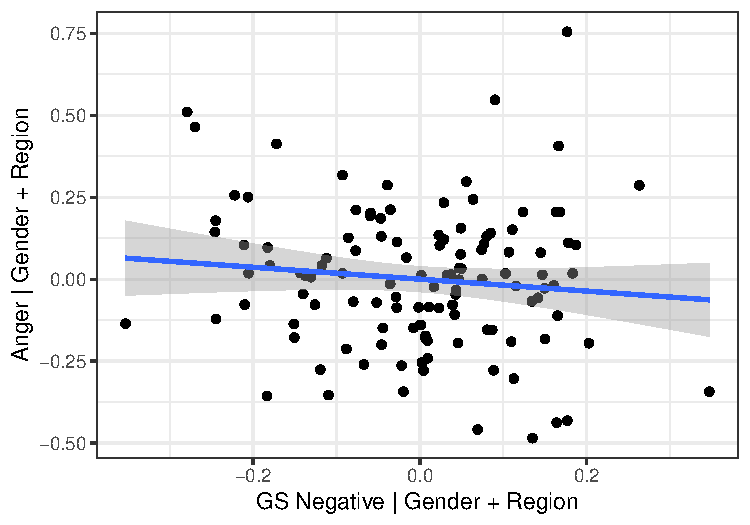
\includegraphics[width=0.48\linewidth]{plots/pcp_anger_GS} }\subfloat[Anxiety GS Negative\label{fig:pcp-plots-2}]{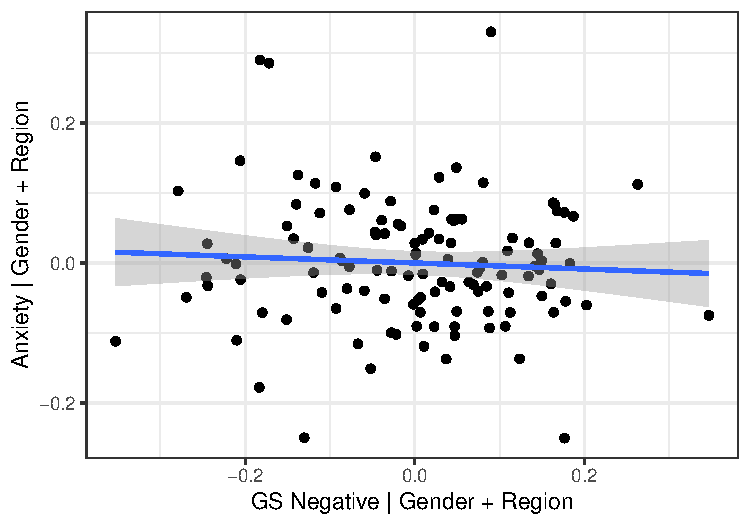
\includegraphics[width=0.48\linewidth]{plots/pcp_anxiety_GS} }\newline\subfloat[Depression GS Negative\label{fig:pcp-plots-3}]{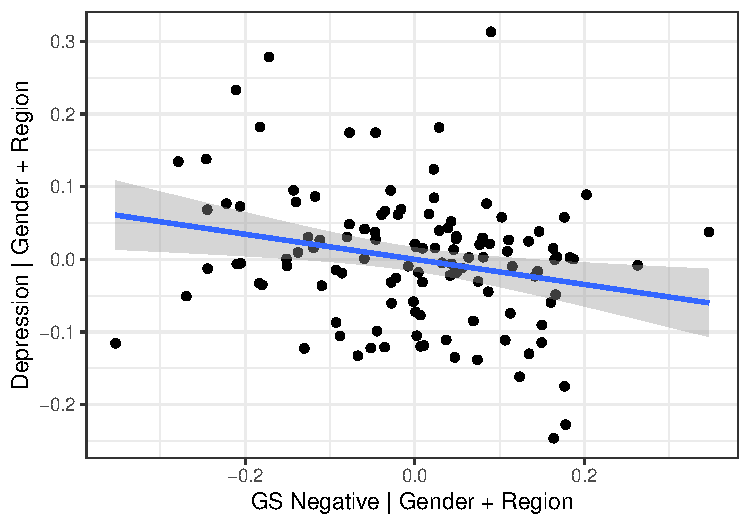
\includegraphics[width=0.48\linewidth]{plots/pcp_depr_GS} }\subfloat[Anger LIWC Anger\label{fig:pcp-plots-4}]{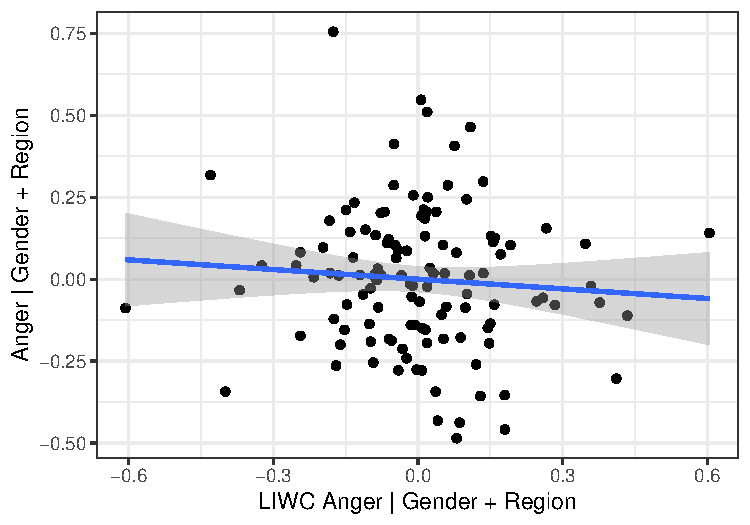
\includegraphics[width=0.48\linewidth]{plots/pcp_anger_LIWC} }\newline\subfloat[Anxiety LIWC Anxiety\label{fig:pcp-plots-5}]{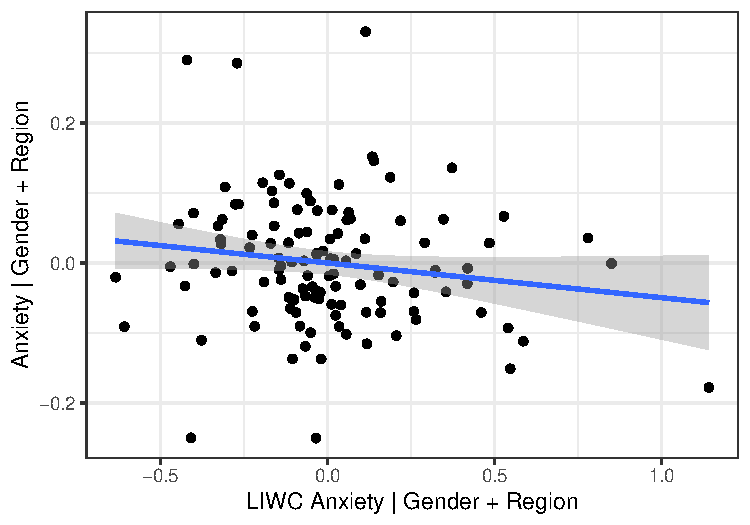
\includegraphics[width=0.48\linewidth]{plots/pcp_anxiety_LIWC} }\subfloat[Depression LIWC Sadness \label{fig:pcp-plots-6}]{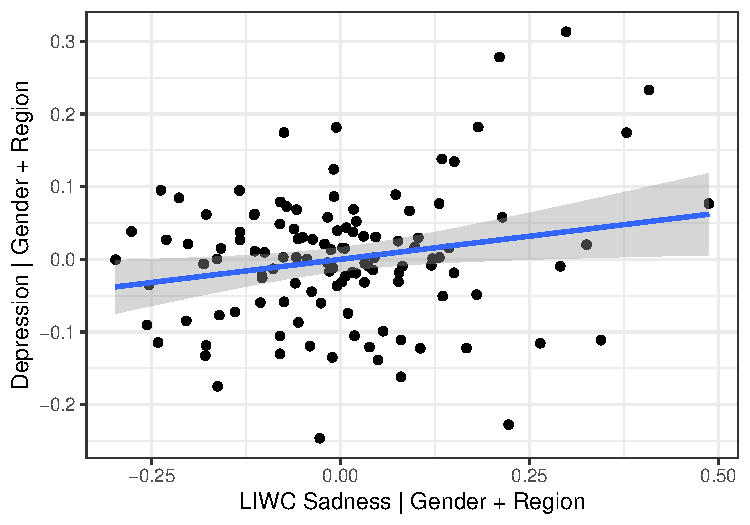
\includegraphics[width=0.48\linewidth]{plots/pcp_depr_LIWC} }

\textit{Note:} The shaded area within the plot represents the 95 \% bootstrapped confidence intervals of the regression line.
\end{figure*}

\begin{figure*}
\caption{Diagnostic Plots \label{fig:diagnostic-plots}}
\subfloat[Anger GS Negative\label{fig:diagnostic-plots-1}]{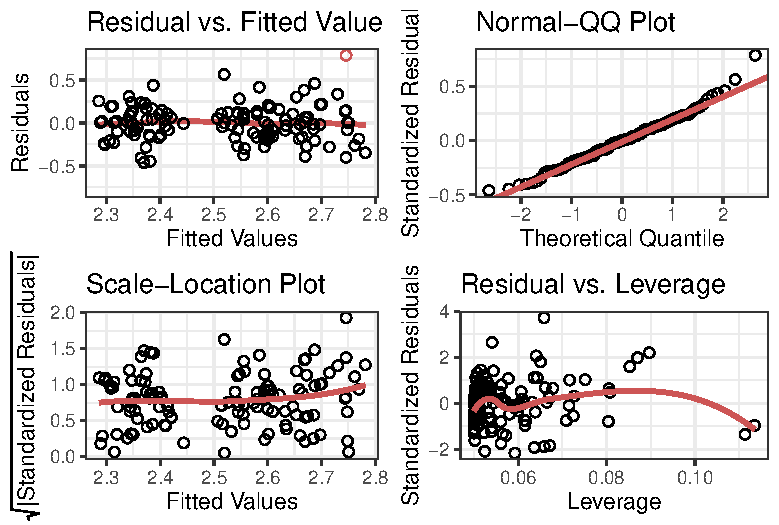
\includegraphics[width=0.48\linewidth]{plots/diagnostic_ang_GS} }\subfloat[Anxiety GS Negative\label{fig:diagnostic-plots-2}]{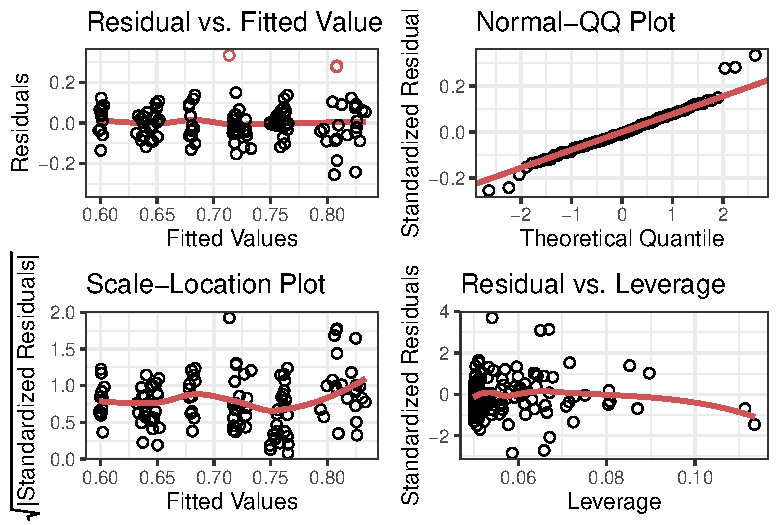
\includegraphics[width=0.48\linewidth]{plots/diagnostic_anx_GS} }\newline\subfloat[Depression GS Negative\label{fig:diagnostic-plots-3}]{\includegraphics[width=0.48\linewidth]{plots/diagnostic_depr_GS} }\subfloat[Anger LIWC Anger\label{fig:diagnostic-plots-4}]{\includegraphics[width=0.48\linewidth]{plots/diagnostic_ang_LIWC} }\newline\subfloat[Anxiety LIWC Anxiety\label{fig:diagnostic-plots-5}]{\includegraphics[width=0.48\linewidth]{plots/diagnostic_anx_LIWC} }\subfloat[Depression LIWC Sadness\label{fig:diagnostic-plots-6}]{\includegraphics[width=0.48\linewidth]{plots/diagnostic_depr_LIWC} }
\end{figure*}

\begin{figure*}
\caption{Spearman's $\rho$ as a Function of the Time Window of Twitter and Der Standard Data Used to Calculate Sentiment Measures}\label{fig:scatter-lag-50}
\subfloat[Twitter\label{fig:scatter-lag-50-1}]{\includegraphics[width=\textwidth]{plots/plt_twitter_lag_50} }\newline\subfloat[Der Standard\label{fig:scatter-lag-50-2}]{\includegraphics[width=\textwidth]{plots/plt_stand_lag_50} }

\textit{Note:} This plot depicts the influence of the time window we used to include social media data for the computation of the sentiment measures on the correlation between self-reported and social media sentiment and emotion measures. The motivation behind this analysis is that the survey questions refer back either 14 days in the case of depression or seven days in case of anxiety and anger. To take this into account the start of the time window of included social media data is likewise adopted to either 14 or seven days prior to each survey wave. Past research indicates that the respondent's memory recall might be biased towards more short-termed events. We thus computed correlations based on restricted time windows. Increased correlations with the survey measures for a shorter time window would underline this theory. Note that for anxiety and anger only the correlations for time windows ranging from one to seven days are relevant. For depression the complete range, i.e., from 14 days to one day is relevant. Compared to Figure~\ref{fig:scatter-lag} we computed these correlations with a reduced dataset. Both social media and survey responses were only included up to the point when 50\,\% of the participants responded to each survey wave.
\end{figure*}

\begin{table*}[h]

\begin{center}
\begin{threeparttable}

\caption{\label{tab:subset-detail}Five Best Models for the Best Subset Selection that Minimized the AIC for Survey Anger}

\small{

\begin{tabular}{lllllllllllll}
\toprule
Salz & \multicolumn{1}{c}{Styr} & \multicolumn{1}{c}{Tyr} & \multicolumn{1}{c}{Vie} & \multicolumn{1}{c}{Male} & \multicolumn{1}{c}{LI Pos} & \multicolumn{1}{c}{LI Neg} & \multicolumn{1}{c}{LI Anx} & \multicolumn{1}{c}{LI Ang} & \multicolumn{1}{c}{LI Sad} & \multicolumn{1}{c}{GS Pos} & \multicolumn{1}{c}{GS Neg} & \multicolumn{1}{c}{AIC}\\
\midrule
0.18 & - & - & - & -0.29 & 0.14 & - & - & -0.32 & 0.59 & -0.19 & - & -384.78\\
0.20 & - & 0.08 & - & -0.29 & 0.09 & - & - & -0.28 & 0.60 & -0.24 & - & -384.53\\
0.19 & - & 0.09 & - & -0.29 & - & - & - & -0.31 & 0.63 & -0.22 & - & -384.06\\
0.17 & - & - & - & -0.29 & - & - & - & -0.36 & 0.64 & -0.16 & - & -383.96\\
0.19 & - & - & - & -0.29 & - & - & - & -0.35 & 0.63 & -0.16 & -0.05 & -383.75\\
\bottomrule
\end{tabular}

}

\end{threeparttable}
\end{center}

\end{table*}

\begin{table*}[h]

\begin{center}
\begin{threeparttable}

\caption{\label{tab:subset-detail-2}Five Best Models for the Best Subset Selection that Minimized the BIC for Survey Anger}

\small{

\begin{tabular}{lllllllllllll}
\toprule
Salz & \multicolumn{1}{c}{Styr} & \multicolumn{1}{c}{Tyr} & \multicolumn{1}{c}{Vie} & \multicolumn{1}{c}{Male} & \multicolumn{1}{c}{LI Pos} & \multicolumn{1}{c}{LI Neg} & \multicolumn{1}{c}{LI Anx} & \multicolumn{1}{c}{LI Ang} & \multicolumn{1}{c}{LI Sad} & \multicolumn{1}{c}{GS Pos} & \multicolumn{1}{c}{GS Neg} & \multicolumn{1}{c}{BIC}\\
\midrule
0.15 & - & - & - & -0.30 & - & - & - & -0.33 & 0.68 & - & - & -370.18\\
0.17 & - & - & - & -0.29 & - & - & - & -0.36 & 0.64 & -0.16 & - & -370.02\\
0.18 & - & - & - & -0.29 & 0.14 & - & - & -0.32 & 0.59 & -0.19 & - & -368.05\\
0.11 & - & - & - & -0.30 & - & - & - & - & 0.59 & - & - & -367.40\\
0.19 & - & 0.09 & - & -0.29 & - & - & - & -0.31 & 0.63 & -0.22 & - & -367.33\\
\bottomrule
\end{tabular}

}

\end{threeparttable}
\end{center}

\end{table*}

\begin{table*}[h]

\begin{center}
\begin{threeparttable}

\caption{\label{tab:subset-detail-3}Five Best Models for the Best Subset Selection that Minimized the AIC for Survey Anxiety}

\small{

\begin{tabular}{lllllllllllll}
\toprule
Salz & \multicolumn{1}{c}{Styr} & \multicolumn{1}{c}{Tyr} & \multicolumn{1}{c}{Vie} & \multicolumn{1}{c}{Male} & \multicolumn{1}{c}{LI Pos} & \multicolumn{1}{c}{LI Neg} & \multicolumn{1}{c}{LI Anx} & \multicolumn{1}{c}{LI Ang} & \multicolumn{1}{c}{LI Sad} & \multicolumn{1}{c}{GS Pos} & \multicolumn{1}{c}{GS Neg} & \multicolumn{1}{c}{AIC}\\
\midrule
0.06 & - & 0.05 & -0.06 & -0.12 & - & 0.18 & -0.06 & - & - & - & - & -571.09\\
0.07 & - & - & -0.05 & -0.12 & - & - & -0.04 & - & - & - & - & -570.56\\
0.08 & - & 0.04 & -0.04 & -0.12 & - & - & -0.02 & - & - & - & - & -570.39\\
0.06 & - & - & -0.06 & -0.12 & - & - & -0.05 & - & 0.08 & - & - & -570.06\\
0.08 & - & - & -0.07 & -0.13 & - & 0.15 & -0.06 & - & - & - & -0.08 & -570.04\\
\bottomrule
\end{tabular}

}

\end{threeparttable}
\end{center}

\end{table*}

\begin{table*}[h]

\begin{center}
\begin{threeparttable}

\caption{\label{tab:subset-detail-4}Five Best Models for the Best Subset Selection that Minimized the BIC for Survey Anxiety}

\small{

\begin{tabular}{lllllllllllll}
\toprule
Salz & \multicolumn{1}{c}{Styr} & \multicolumn{1}{c}{Tyr} & \multicolumn{1}{c}{Vie} & \multicolumn{1}{c}{Male} & \multicolumn{1}{c}{LI Pos} & \multicolumn{1}{c}{LI Neg} & \multicolumn{1}{c}{LI Anx} & \multicolumn{1}{c}{LI Ang} & \multicolumn{1}{c}{LI Sad} & \multicolumn{1}{c}{GS Pos} & \multicolumn{1}{c}{GS Neg} & \multicolumn{1}{c}{BIC}\\
\midrule
0.09 & - & 0.06 & - & -0.12 & - & - & - & - & - & - & - & -559.83\\
0.06 & - & - & -0.06 & -0.12 & - & - & - & - & - & - & - & -559.78\\
0.07 & - & - & -0.05 & -0.12 & - & - & -0.04 & - & - & - & - & -559.41\\
0.08 & - & - & - & -0.12 & - & - & -0.05 & - & - & - & - & -558.67\\
0.07 & - & 0.04 & -0.04 & -0.12 & - & - & - & - & - & - & - & -558.40\\
\bottomrule
\end{tabular}

}

\end{threeparttable}
\end{center}

\end{table*}

\begin{table*}[h]

\begin{center}
\begin{threeparttable}

\caption{\label{tab:subset-detail-5}Five Best Models for the Best Subset Selection that Minimized the AIC for Survey Depression}

\small{

\begin{tabular}{lllllllllllll}
\toprule
Salz & \multicolumn{1}{c}{Styr} & \multicolumn{1}{c}{Tyr} & \multicolumn{1}{c}{Vie} & \multicolumn{1}{c}{Male} & \multicolumn{1}{c}{LI Pos} & \multicolumn{1}{c}{LI Neg} & \multicolumn{1}{c}{LI Anx} & \multicolumn{1}{c}{LI Ang} & \multicolumn{1}{c}{LI Sad} & \multicolumn{1}{c}{GS Pos} & \multicolumn{1}{c}{GS Neg} & \multicolumn{1}{c}{AIC}\\
\midrule
0.12 & 0.06 & - & -0.03 & -0.17 & - & 0.44 & -0.11 & -0.20 & - & - & -0.17 & -580.34\\
0.13 & 0.07 & - & - & -0.17 & - & 0.41 & -0.10 & -0.22 & - & - & -0.16 & -580.17\\
0.13 & 0.08 & 0.04 & - & -0.17 & - & 0.47 & -0.11 & -0.23 & - & - & -0.12 & -580.12\\
0.11 & 0.05 & - & -0.03 & -0.17 & 0.07 & 0.42 & -0.11 & -0.18 & - & - & -0.14 & -579.39\\
0.12 & 0.06 & - & - & -0.17 & 0.08 & 0.39 & -0.11 & -0.20 & - & - & -0.13 & -579.33\\
\bottomrule
\end{tabular}

}

\end{threeparttable}
\end{center}

\end{table*}

\begin{table*}[tbp]

\begin{center}
\begin{threeparttable}

\caption{\label{tab:subset-detail-6}Five Best Models for the Best Subset Selection that Minimized the BIC for Survey Depression}

\small{

\begin{tabular}{lllllllllllll}
\toprule
Salz & \multicolumn{1}{c}{Styr} & \multicolumn{1}{c}{Tyr} & \multicolumn{1}{c}{Vie} & \multicolumn{1}{c}{Male} & \multicolumn{1}{c}{LI Pos} & \multicolumn{1}{c}{LI Neg} & \multicolumn{1}{c}{LI Anx} & \multicolumn{1}{c}{LI Ang} & \multicolumn{1}{c}{LI Sad} & \multicolumn{1}{c}{GS Pos} & \multicolumn{1}{c}{GS Neg} & \multicolumn{1}{c}{BIC}\\
\midrule
0.07 & - & - & - & -0.15 & 0.23 & - & - & - & - & - & - & -567.20\\
0.08 & - & - & - & -0.15 & 0.21 & - & -0.07 & - & - & - & - & -566.52\\
0.13 & 0.07 & - & - & -0.17 & - & 0.41 & -0.10 & -0.22 & - & - & -0.16 & -564.52\\
0.09 & 0.05 & - & - & -0.15 & - & - & - & -0.19 & 0.16 & - & - & -564.16\\
0.10 & 0.06 & - & - & -0.16 & - & - & -0.08 & -0.15 & 0.18 & - & - & -563.96\\
\bottomrule
\addlinespace
\end{tabular}

}

\begin{tablenotes}[para]
\normalsize{\textit{Note.} Salz, Styr, Tyr and Vie are abbreviations for Salzburg, Styria, Tyrol and Vienna. LI, Pos, Neg, Anx, Ang and Depr are the respective abbreviations for LIWC, positive, negative, anxiety, anger, and depression. A hyphen indicates that the corresponding variable was not included in the model.}
\end{tablenotes}

\end{threeparttable}
\end{center}

\end{table*}

\begin{figure*}[h!]
\caption{Mixed Correlations between the Included Survey Variables in the Factor Analysis}\label{fig:table-mix-cor}
\includegraphics[width=\textwidth]{plots/plot_mixed_cor} 

\textit{Note:} Mixed refers to the fact that the correlations were not computed by Pearson's correlation. Instead we considered the scale of the variables and hence computed tetrachoric, polychoric or polyserial correlations.
\end{figure*}

\begin{figure*}[h!]
\caption{Scree Plot of Factor Analysis}\label{fig:scree-plot}
\includegraphics[width=\textwidth]{plots/scree_plot} 

\textit{Note:} According to the scree plot, factors to the left of the plot's "ellbow" are retained. In this case, the scree plot suggests to include two factors. The blue dashed line shows the results of the parallel analysis. With this approach, all factors up to the first eigenvalue of the simulated data that exceeds the corresponding eigenvalue of the actual data should be retained. Contrarily to the scree plot, parallel analsis suggests to include six factors.
\end{figure*}

\begin{table*}[tbp]

\begin{center}
\begin{threeparttable}

\caption{\label{tab:loading}Loading Structure and Communalities after Varmiax Rotation}

\small{

\begin{tabular}{llll}
\toprule
 & \multicolumn{1}{c}{Positive Life Outcome Score} & \multicolumn{1}{c}{Conflict- and Suicide-Related Score} & \multicolumn{1}{c}{Communality}\\
\midrule
Conflicts family/partner & 0.07 & 0.71 & 0.50\\
Conflicts work & 0.11 & 0.67 & 0.46\\
Psychological domestic violence & 0.09 & 0.92 & 0.85\\
Physical domestic violence & 0.04 & 0.88 & 0.77\\
Change conflict & -0.17 & 0.33 & 0.14\\
Suicidal thoughts & -0.02 & 0.53 & 0.28\\
More wellbeing & 0.71 & 0.09 & 0.51\\
More relaxed & 0.77 & 0.02 & 0.60\\
Less stress & 0.67 & -0.08 & 0.46\\
Happier & 0.82 & 0.01 & 0.67\\
More connected & 0.27 & -0.13 & 0.09\\
More family & 0.60 & 0.10 & 0.36\\
More friends & 0.57 & 0.14 & 0.34\\
More hobbies & 0.58 & -0.06 & 0.34\\
Less boredom & 0.45 & 0.15 & 0.23\\
More sport & 0.48 & 0.00 & 0.23\\
Healthier nutrition & 0.45 & -0.10 & 0.21\\
Better sleep & 0.74 & -0.01 & 0.54\\
\bottomrule
\end{tabular}

}

\end{threeparttable}
\end{center}

\end{table*}


\end{document}
